\documentclass{article}

% !TEX root =  tb_icml_2018.tex

\PassOptionsToPackage{compress}{natbib}
\usepackage[accepted]{icml2018}

\usepackage{tikz}
\usetikzlibrary{fit}					% fitting shapes to coordinates
\usetikzlibrary{backgrounds}	% drawing the background after the foreground


\usepackage{url}
\usepackage{amsmath}
\usepackage{amssymb}
\usepackage{amsbsy}
\usepackage{siunitx}
%\usepackage{algorithm}
%\usepackage{algorithmicx}
%\usepackage{algpseudocode}
\usepackage{mathtools}
\usepackage{array}
\usepackage{setspace}
\usepackage{caption}
\usepackage{subcaption}
\usepackage{booktabs}
\usepackage{adjustbox}
\usepackage{microtype}

\usepackage{todonotes}

\usepackage{wrapfig}
\usepackage{tabularx}

\usepackage{times}
\usepackage[bottom]{footmisc}
\usepackage{listings}
\usepackage{color}
\usepackage{xcolor}
\usepackage{textcomp}
\usepackage{xspace}

\usepackage{amsthm}

\usepackage{bbm}


\usepackage{thmtools}
\usepackage{thm-restate}
\usepackage{cancel}

%\usepackage{hyperref}

%\bibliographystyle{icml2017}
%\bibliographystyle{abbrvnat-simple}
\bibliographystyle{icml2017}
\setlength{\bibsep}{2.5pt}
%\setlength{\bibsep}{5.0pt}

\usepackage{todonotes}
%\newcommand{\E}{\mathbb{E}}

\theoremstyle{plain}
\newtheorem{theorem}{Theorem}

\theoremstyle{plain}
\newtheorem{theoremApp}{Theorem}

\theoremstyle{remark}
\newtheorem{remark}{Remark}

\theoremstyle{lemma}
\newtheorem{lemma}{Lemma}

\theoremstyle{corollary}
\newtheorem{corollary}{Corollary}

\newcommand{\tom}[1] {{\textcolor{red}{#1}}}

\graphicspath{{../figures/}}

\usepackage{paralist}

\usepackage{thmtools}
\usepackage{thm-restate}

\usepackage{multicol}

\usepackage{wrapfig}

\newcommand{\E}{\mathbb{E}}

\definecolor{darkgreenClj}{rgb}{0.25,.5,0.25}
\definecolor{blueClj}{rgb}{0,0.33,0.66}
\definecolor{redClj}{rgb}{0.66,0.0,0.0}
\definecolor{purpleClj}{rgb}{0.33,0,0.66}
\definecolor{cyanClj}{rgb}{0.0,0.5,0.5}
\definecolor{orangeClj}{rgb}{0.75,0.35,0.0}
\definecolor{grayClj}{rgb}{0.4,0.4,0.4}
\lstset{
	language=Lisp,
	basicstyle=\small\ttfamily,
	keywordstyle={},
	alsoletter={<-,->,:,*,/,?,+,-,/,>,<,=, &},
	commentstyle=\em \color{gray},
	frame=lines,
	%float=tbph,
	% captionpos=b,
	showstringspaces=false,
	keywordstyle=[1]\bf\ttfamily\color{blueClj},
	keywords=[1]{BO,theta-best,bo-acquire,sample-initial-points,sample,observe,observe<-,predict,mem,store,retrieve,return,catch,throw,absorb,produce,with-primitive-procedures,conditional,result,log-marginal,mean,
		->sample,->observe,->result},
	keywordstyle=[2]\bf\ttfamily\color{redClj},
	keywords=[2]{if,let,letfn,loop,looppredict,recur,or,trampoline,assoc,argmax,count,cons,conj,
		do,first,fn,get,keys,lazy-seq,map,nth,mat/add,mat/div,print,reduce,repeat,repeatedly,rest,set,shape,take,vec,
		when,max,fn?,inc,sample*,observe*},
	keywordstyle=[3]\bf\ttfamily\color{cyanClj},
	keywords=[3]{dirichlet-discrete,exponential,flip,gamma,beta,mvn-niw,normal,uniform-continuous,distribution,factor,
		simulate,abc-likelihood,student-t,dirichlet},
	keywordstyle=[4]\bf\ttfamily\color{purpleClj},
	keywords=[4]{defopt,defquery,doopt,doquery,query,defdist,infer,checkpoint,exec,defm,cps-of-expression,
		defn,def,declare},
	keywordstyle=[5]\bf\ttfamily\color{orangeClj},
	keywords=[5]{:lmh,:ipmcmc,:war,:peace,:log-weight,:result,:id,:dist,:cont,:value,:state,:importance,:smc,:pgibbs},
	mathescape=true,
	stringstyle={},
	keywordstyle=[6]\bf\ttfamily\color{darkgreenClj},
	keywords=[6]{+,-,nil,>,<,*,/,=, &,->>,->},
	mathescape=true,
	stringstyle={},
}
\lstnewenvironment{code}[2]{\lstset{caption=#1,label=#2}}{}

%\newtheorem{example}{Example}
%%\newtheorem{theorem}{Theorem}[chapter]
%\newtheorem{lemma}[theorem]{Lemma}
%%\newtheorem{proposition}[proposition]{Proposition}
%\newtheorem{remark}{Remark}[chapter]
%%\newtheorem{corollary}[corollary]{Corollary}
%\newtheorem{definition}{Definition}[chapter]
%\newtheorem{conjecture}[conjecture]{Conjecture}
%\newtheorem{axiom}[axiom]{Axiom}

% % % % % % % % % % % % % % % % % % %


%\usepackage{packages/algorithm,packages/algorithmic}
\usepackage{abbreviations}

%\usepackage{algorithmicx}
%\usepackage{algpseudocode}
%\usepackage{setspace}
%% % % % % % % % %
%\algnewcommand\algorithmicswitch{\textbf{switch}}
%\algnewcommand\algorithmiccase{\textbf{case}}
%\algnewcommand\algorithmicassert{\texttt{assert}}
%\algnewcommand\Assert[1]{\State \algorithmicassert(#1)}%
%% New "environments"
%\algdef{SE}[SWITCH]{Switch}{EndSwitch}[1]{\algorithmicswitch\ #1\ \algorithmicdo}{\algorithmicend\ \algorithmicswitch}%
%\algdef{SE}[CASE]{Case}{EndCase}[1]{\algorithmiccase\ #1}{\algorithmicend\ \algorithmiccase}%
%%\algtext*{EndSwitch}%
%\algtext*{EndCase}%
%\algnewcommand{\IIf}[1]{\State\algorithmicif\ #1\ \algorithmicthen}
%\algnewcommand{\EndIIf}{\unskip\ \algorithmicend\ \algorithmicif}
%
\usepackage{titlesec}
\titlespacing\section{0pt}{4pt plus 2pt minus 2pt}{0pt plus 2pt minus 0pt}
\titlespacing\subsection{0pt}{4pt plus 2pt minus 2pt}{0pt plus 2pt minus 0pt}
\titlespacing\subsubsection{0pt}{4pt plus 2pt minus 2pt}{0pt plus 2pt minus 0pt}

\usepackage[acronym,smallcaps,nowarn,section,nogroupskip,nonumberlist]{glossaries}
\newacronym{VAE}{vae}{variational auto-encoder}
\newacronym{AESMC}{aesmc}{auto-encoding sequential Monte Carlo}
\newacronym{IS}{is}{importance sampling}
\newacronym{IWAE}{iwae}{importance-weighted auto-encoder}
\newacronym{PIWAE}{piwae}{partially importance-weighted auto-encoder}
\newacronym{MIWAE}{miwae}{multiply importance-weighted auto-encoder}
\newacronym{CIWAE}{ciwae}{combination importance-weighted auto-encoder}
\newacronym{SMC}{smc}{sequential Monte Carlo}
\newacronym{SSM}{ssm}{state-space model}
\newacronym{SGA}{sga}{stochastic gradient ascent}
\newacronym{SGD}{sgd}{stochastic gradient descent}
\newacronym{ELBO}{elbo}{evidence lower bound}
\newacronym{KL}{kl}{Kullback-Leibler}
\newacronym{LSTM}{lstm}{long short-term memory}
\newacronym{AD}{ad}{automatic differentiation}
\newacronym{SPSA}{spsa}{simultaneous perturbation stochastic approximation}
\newacronym{CG-SPSA}{cg-spsa}{computational graph SPSA}
\newacronym{MML}{mml}{maximum marginal likelihood}
\newacronym{REINFORCE}{reinforce}{REINFORCE}
\glsunset{REINFORCE}
\newacronym{ADAM}{adam}{ADAM}
\glsunset{ADAM}
\newacronym{GRU}{gru}{gated recurrent unit}
\newacronym{MLP}{mlp}{multilayer perceptron}
\newacronym{MAP}{map}{maximum a-posteriori}
\newacronym{KDE}{kde}{kernel density estimation}
\newacronym{EM}{em}{expectation maximization}
\newacronym{MC}{mc}{Monte Carlo}
\newacronym{ALT}{alt}{alternating \textsc{elbo}s}
\newacronym{SNR}{snr}{signal-to-noise ratio}
\newacronym{VRNN}{vrnn}{Variational Recurrent Neural Network}
\newacronym{LGSSM}{lgssm}{linear Gaussian state space model}
\newacronym[firstplural=recurrent neural networks, plural=RNNs]{RNN}{rnn}{recurrent neural network}
\newacronym{MCM}{mcmc}{Markov Chain Monte Carlo}
\newacronym{RMSE}{rmse}{root mean squared error}

\newcommand{\given}{\lvert}
\DeclareMathOperator{\Var}{\mathbb{V}}
\DeclareMathOperator{\Bernoulli}{\mathrm{Bernoulli}}
\DeclareMathOperator{\ELBO}{\acrshort{ELBO}}
\DeclareMathOperator{\SNR}{\acrshort{SNR}}
\DeclareMathOperator*{\maximize}{maxi\,\!mize}
\newcommand{\KL}[2]{\acrshort{KL}\left(#1 \middle| \middle| #2\right)}


\usepackage{fancyhdr}
%\pagenumbering{arabic} 
%\pagestyle{fancy}
%\cfoot{\vspace*{1.5\baselineskip} \thepage}

\setlength{\parskip}{0.2em}

% The \icmltitle you define below is probably too long as a header.
% Therefore, a short form for the running title is supplied here:
\icmltitlerunning{Tighter Variational Bounds are Not Necessarily Better}


\usepackage{xr,refcount}
\usepackage{chngcntr}
\externaldocument{tb_icml_2018}

\begin{document}
%
%	\vspace{-20pt}

	
\twocolumn[
\icmltitle{Tighter Variational Bounds are Not Necessarily Better}

% It is OKAY to include author information, even for blind
% submissions: the style file will automatically remove it for you
% unless you've provided the [accepted] option to the icml2018
% package.

% List of affiliations: The first argument should be a (short)
% identifier you will use later to specify author affiliations
% Academic affiliations should list Department, University, City, Region, Country
% Industry affiliations should list Company, City, Region, Country

% You can specify symbols, otherwise they are numbered in order.
% Ideally, you should not use this facility. Affiliations will be numbered
% in order of appearance and this is the preferred way.
\icmlsetsymbol{equal}{*}

\begin{icmlauthorlist}
	\icmlauthor{Tom Rainforth}{stats}
\icmlauthor{Adam R. Kosiorek}{stats,eng}
\icmlauthor{Tuan Anh Le}{eng}
\icmlauthor{Chris J. Maddison}{stats}
\icmlauthor{Maximilian Igl}{eng}
\icmlauthor{Frank Wood}{ucb}
\icmlauthor{Yee Whye Teh}{stats}
\end{icmlauthorlist}

\icmlaffiliation{stats}{Department of Statistics, University of Oxford}
\icmlaffiliation{eng}{Department of Engineering, University of Oxford}
\icmlaffiliation{ucb}{Department of Computer Science, University of British Columbia}

\icmlcorrespondingauthor{Tom Rainforth}{rainforth@stats.ox.ac.uk}

% You may provide any keywords that you
% find helpful for describing your paper; these are used to populate
% the "keywords" metadata in the PDF but will not be shown in the document
\icmlkeywords{Variational inference, variational autoencoders, importance weighted autoencoders}

\vskip 0.3in
]
\printAffiliationsAndNotice{}	

%
\setlength{\abovedisplayskip}{2.5pt}
\setlength{\belowdisplayskip}{2.5pt}
\setlength{\abovedisplayshortskip}{2.5pt}
\setlength{\belowdisplayshortskip}{2.5pt}
%
%\vspace{-8pt}

\begin{abstract}
%	\vspace{-8pt}
%Recent work on variational objectives for deep generative models often makes the implicit assumption that tighter evidence bounds (ELBOs) are better objectives.  
\vspace{2pt}
We provide theoretical and empirical evidence that using tighter \glspl{ELBO}
can be
detrimental to the process of learning an inference network by reducing the 
signal-to-noise ratio of the gradient estimator.  Our results call into question common 
implicit assumptions that tighter \glspl{ELBO} are better variational objectives for 
simultaneous model learning and inference amortization schemes.
Based on our insights, we introduce three new algorithms:  the partially importance
weighted auto-encoder (\textsc{piwae}), the multiply
importance weighted auto-encoder (\textsc{miwae}), and the combination importance weighted
auto-encoder (\textsc{ciwae}), each of which includes the standard importance
weighted auto-encoder (\textsc{iwae}) as a special case.  We show that each
can deliver improvements over \textsc{iwae}, even when performance is measured
by the \textsc{iwae} target itself. Furthermore, our results suggest that \textsc{piwae} 
may be able to deliver simultaneous improvements in the training of both
the inference and generative networks.
%, suggesting that 
%further investigation
%is required to assess the relative utility of different approaches.  
% Based on our
%insights, we introduce a new approach for training deep generative models, the 
%partially importance-weighted auto-encoder (\textsc{piwae}), that uses different objectives for
%training the generative and inference networks.  These objectives can be simply estimated
%using a common set of samples and, despite only requiring minimal algorithmic changes
%to previous approaches, can provide substantial improvements to the learning process.
%\vspace{-8pt}
\end{abstract}

%\vspace{-15pt}


%\section{Conclusions and Future Work}


\clearpage

\section*{Acknowledgments}

TR and YWT are supported in part by the European Research Council under the European Union's Seventh Framework Programme (FP7/2007--2013) / ERC grant agreement no. 617071. 
TAL is supported by a Google studentship, project code DF6700.
MI is supported by the UK EPSRC CDT in Autonomous Intelligent Machines
and Systems.
CJM is funded by a DeepMind Scholarship.
FW is supported under DARPA PPAML through the U.S. AFRL
under Cooperative Agreement FA8750-14-2-0006, Sub Award number 61160290-111668.



\clearpage

\appendix
	\onecolumn
\setlength{\abovedisplayskip}{5pt}
\setlength{\belowdisplayskip}{5pt}
\setlength{\abovedisplayshortskip}{5pt}
\setlength{\belowdisplayshortskip}{5pt}

\titlespacing\section{0pt}{8pt plus 2pt minus 2pt}{2pt plus 2pt minus 0pt}
\titlespacing\subsection{0pt}{8pt plus 2pt minus 2pt}{2pt plus 2pt minus 0pt}
\titlespacing\subsubsection{0pt}{8pt plus 2pt minus 2pt}{2pt plus 2pt minus 0pt}

\thispagestyle{empty} 
\rule{\textwidth}{1pt}
\vspace{-6pt}
\begin{center}
	\textbf{ \Large  Appendices for Tighter Variational Bounds are Not Necessarily
		Better}
\end{center}%\vspace{-6pt}
\rule{\textwidth}{1pt}

	\begin{minipage}{\textwidth}
		\centering
		\vspace{17pt}
		\textbf{Tom Rainforth \quad Adam R. Kosiorek \quad Tuan Anh Le \quad Chris J. Maddison \\
		 Maximilian Igl \quad Frank Wood \quad Yee Whye Teh}
		\vspace{6pt}
	\end{minipage}
	
\renewcommand{\theequation}{\thesection.\arabic{equation}}  
\renewcommand\thefigure{\thesection.\arabic{figure}}  
\counterwithin{figure}{section}

\section{Proof of SNR Convergence Rates}
\label{sec:proof}

\begin{theoremApp}
	\label{the:app:snr}
	Assume that when $M=K=1$, the expected gradients; the variances of the gradients; and the 
	first four moments of  $w_{1,1}$, $\nabla_{\theta} w_{1,1}$, and 
	$\nabla_{\phi} w_{1,1}$ are all finite and the variances are
	also non-zero.
	Then the signal-to-noise ratios of the gradient estimates converge at the following rates
	\begin{align}
	\SNR_{M,K} (\theta) &= 
	\sqrt{M}\left|\frac{ \sqrt{K} \; 
		\nabla_{\theta} Z -\frac{1}{2Z\sqrt{K}}\nabla_{\theta} \left(\frac{\textnormal{Var} \left[w_{1,1}\right]}{Z^2}\right)+ O\left(\frac{1}{K^{3/2}}\right) }
	{\sqrt{\E \left[w_{1,1}^2\left(\nabla_{\theta} \log w_{1,1}-\nabla_{\theta} \log Z\right)^2\right]} + O\left(\frac{1}{K}\right)}\right| \\
	\SNR_{M,K} (\phi) & =\sqrt{M} \left|\frac{
		\nabla_{\phi} \textnormal{Var} \left[w_{1,1}\right] + O\left(\frac{1}{K}\right) }
	{2 Z\sqrt{K} \; \sigma\left[\nabla_{\phi} w_{1,1}\right] +O\left(\frac{1}{\sqrt{K}}\right)}\right|
	\end{align}
	where $Z := p_{\theta}(x)$ is the true marginal likelihood.
\end{theoremApp}

\begin{proof}
We start by considering the variance of the estimators.   We will first exploit the 
fact that each $\hat{Z}_{m,K}$ is independent and identically distributed and then apply
Taylor's theorem\footnote{This approach follows similar lines
	to the derivation of nested Monte Carlo convergence bounds in~\cite{Rainforth2017thesis,Rainforth2017opportunities,Fort2017mcmc}
and the derivation of the mean squared error for self-normalized
importance sampling, see e.g.~\cite{Hesterberg1988advances}.}
to 
$\log \hat{Z}_{m,K}$ about $Z$, using $R_1(\cdot)$ to indicate the remainder term, as
follows.
\begin{align*}
M& \cdot \text{Var} \left[\Delta_{M,K}\right] = \text{Var} \left[\Delta_{1,K}\right]
=\text{Var} \left[\nabla_{\theta,\phi} \left( 
\log Z + \frac{\hat{Z}_{1,K}-Z}{Z} + R_1\left(\hat{Z}_{1,K}\right)
\right)\right] \displaybreak[0] \\
=& \text{Var} \left[\nabla_{\theta,\phi} \left( 
\frac{\hat{Z}_{1,K}-Z}{Z} + R_1\left(\hat{Z}_{1,K}\right)
\right)\right] \displaybreak[0] \\
=& \E \left[\left(\nabla_{\theta,\phi} \left( 
\frac{\hat{Z}_{1,K}-Z}{Z} + R_1\left(\hat{Z}_{1,K}\right)
\right)\right)^2\right] -  \left(\E \left[\nabla_{\theta,\phi} \left( 
\frac{\hat{Z}_{1,K}-Z}{Z} + R_1\left(\hat{Z}_{1,K}\right)
\right)\right]\right)^2 \displaybreak[0]\\
=&\E \left[\left(\frac{1}{K} \sum_{k=1}^{K} \frac{Z \nabla_{\theta,\phi} w_{1,k}-w_{1,k}\nabla_{\theta,\phi} Z}{Z^2}
+ \nabla_{\theta, \phi} R_1\left(\hat{Z}_{1,K}\right)\right)^2\right]
-  \left(\nabla_{\theta,\phi} \cancelto{0}{\E \left[
	\frac{\hat{Z}_{1,K}-Z}{Z}\right]} + \E \left[ \nabla_{\theta, \phi} R_1\left(\hat{Z}_{1,K}\right)\right]\right)^2 \displaybreak[0]\\
=&\frac{1}{KZ^4} \E \left[\left(Z \nabla_{\theta,\phi} w_{1,1}-w_{1,1}\nabla_{\theta,\phi} Z\right)^2\right] + \text{Var} \left[ \nabla_{\theta, \phi} R_1\left(\hat{Z}_{1,K}\right)\right] \\
&+ 2\E \left[\left(\nabla_{\theta, \phi} R_1\left(\hat{Z}_{1,K}\right)\right)
\left(\frac{1}{K} \sum_{k=1}^{K} \frac{Z \nabla_{\theta,\phi} w_{1,k}-w_{1,k}\nabla_{\theta,\phi} Z}{Z^2}\right)\right]
\end{align*}
Now we have by the mean-value form of the remainder that for some
$\tilde{Z}$ between $Z$ and $\hat{Z}_{1,K}$
\begin{align*}
R_1\left(\hat{Z}_{1,K}\right) = -\frac{\left(\hat{Z}_{1,K}-Z\right)^2}{2 \tilde{Z}^2}
\end{align*}
and therefore
\begin{align*}
\nabla_{\theta,\phi} R_1\left(\hat{Z}_{1,K}\right)
=-\frac{\tilde{Z}\left(\hat{Z}_{1,K}-Z\right)\nabla_{\theta,\phi} \left(\hat{Z}_{1,K}-Z\right)
	-\left(\hat{Z}_{1,K}-Z\right)^2 \nabla_{\theta,\phi}\tilde{Z}}{\tilde{Z}^3}.
\end{align*}
It follows that the $\nabla_{\theta,\phi} R_1\left(\hat{Z}_{1,K}\right)$ terms are
dominated as each of $\left(\hat{Z}_{1,K}-Z\right)\nabla_{\theta,\phi} \left(\hat{Z}_{1,K}-Z\right)$
and $\left(\hat{Z}_{1,K}-Z\right)^2$ vary with the square of the estimator error, whereas
other comparable terms vary only with the unsquared difference.  The assumptions on
moments of the weights and their derivatives further guarantee that these terms are finite.
More precisely, we have $\tilde{Z} = Z+\alpha (\hat{Z}_{1,K}-Z)$ for some
$0<\alpha<1$ where $\nabla_{\theta,\phi} \alpha$ must be bounded with 
probability $1$ as $K\to\infty$ to
maintain our assumptions.  It follows that $\nabla_{\theta,\phi} R_1(\hat{Z}_{1,K}) = O((\hat{Z}_{1,K}-Z)^2)$ and thus that
\begin{align}
\label{eq:var}
\text{Var} \left[\Delta_{M,K}\right] = 
\frac{1}{MKZ^4} \E \left[\left(Z \nabla_{\theta,\phi} w_{1,1}-w_{1,1}\nabla_{\theta,\phi} Z\right)^2\right]
+\frac{1}{M}O\left(\frac{1}{K^2}\right)
\end{align}
using the  fact that the third and fourth order moments of a Monte Carlo 
estimator both decrease at a rate $O(1/K^2)$.

Considering now the expected gradient estimate and again using Taylor's theorem, this
time to a higher number of terms,
\begin{align}
\E \left[\Delta_{M,K}\right] &= \E \left[\Delta_{1,K}\right]
= \E \left[\Delta_{1,K}-\nabla_{\theta,\phi} \log Z\right] +
\nabla_{\theta,\phi} \log Z\displaybreak[0] \nonumber \\ &= 
\nabla_{\theta,\phi} \E \left[\log Z + \frac{\hat{Z}_{1,K}-Z}{Z} 
- \frac{\left(\hat{Z}_{1,K}-Z\right)^2}{2Z^2} + R_2\left(\hat{Z}_{1,K}\right)-\log Z\right]
+
\nabla_{\theta,\phi} \log Z \displaybreak[0] \nonumber \\
&= 
-\frac{1}{2}\nabla_{\theta,\phi} \E \left[\left(\frac{\hat{Z}_{1,K}-Z}{Z}\right)^2\right]+
\nabla_{\theta,\phi} \E \left[R_2\left(\hat{Z}_{1,K}\right)\right] +\nabla_{\theta,\phi} \log Z \displaybreak[0] \nonumber \\
&= -\frac{1}{2}\nabla_{\theta,\phi} \left(\frac{\text{Var} \left[\hat{Z}_{1,K}\right]}{Z^2}\right)
+\nabla_{\theta,\phi} \E \left[R_2\left(\hat{Z}_{1,K}\right)\right] +\nabla_{\theta,\phi} \log Z \displaybreak[0] \nonumber \\
&= -\frac{1}{2K}\nabla_{\theta,\phi} \left(\frac{\text{Var} \left[w_{1,1}\right]}{Z^2}\right)
+\nabla_{\theta,\phi} \E \left[R_2\left(\hat{Z}_{1,K}\right)\right]+\nabla_{\theta,\phi} \log Z . \label{eq:mean}
\end{align}
Using a similar process as in variance case, it is now straightforward to show that
$\nabla_{\theta,\phi} \E \left[R_2\left(\hat{Z}_{1,K}\right)\right]=O(1/K^2)$, which is
thus similarly dominated (also giving us~\eqref{eq:expt}).

Finally, by combing~\eqref{eq:var} and~\eqref{eq:mean} and noting that
$\sqrt{\frac{A}{K}+\frac{B}{K^2}} = \frac{A}{\sqrt{K}}+\frac{B}{2AK^{3/2}}+O\left(\frac{1}{K^{(5/2)}}\right)$ we have
\begin{align}
\SNR_{M,K} (\theta)
&= \left|\frac{\nabla_{\theta} \log Z-\frac{1}{2K}\nabla_{\theta} \left(\frac{\text{Var} \left[w_{1,1}\right]}{Z^2}\right)
	+O\left(\frac{1}{K^2}\right)}
{\sqrt{\frac{1}{MKZ^4} \E \left[\left(Z \nabla_{\theta} w_{1,1}-w_{1,1}\nabla_{\theta} Z\right)^2\right]
	+\frac{1}{M}O\left(\frac{1}{K^2}\right)}}\right| 
\\ &= \sqrt{M}\left|\frac{Z^2\sqrt{K}
	\left(\nabla_{\theta} \log Z -\frac{1}{2K}\nabla_{\theta} \left(\frac{\text{Var} \left[w_{1,1}\right]}{Z^2}\right)\right) 
	+ O\left(\frac{1}{K^{3/2}}\right) }
{\sqrt{\E \left[\left(Z \nabla_{\theta} w_{1,1}-w_{1,1}\nabla_{\theta} Z\right)^2\right]} +O\left(\frac{1}{K}\right)}\right| 
\displaybreak[0] \\
&= \sqrt{M}\left|\frac{ \sqrt{K} \; 
	\nabla_{\theta} Z -\frac{1}{2Z\sqrt{K}}\nabla_{\theta} \left(\frac{\text{Var} \left[w_{1,1}\right]}{Z^2}\right)+ O\left(\frac{1}{K^{3/2}}\right) }
{\sqrt{\E \left[w_{1,1}^2\left(\nabla_{\theta} \log w_{1,1}-\nabla_{\theta} \log Z\right)^2\right]} + O\left(\frac{1}{K}\right)}\right| =O\left(\sqrt{MK}\right).
\end{align}
For $\phi$, then because $\nabla_{\phi} Z = 0$, we instead have
\begin{align}
\SNR_{M,K} (\phi) = \sqrt{M} \left|\frac{
	\nabla_{\phi} \text{Var} \left[w_{1,1}\right] + O\left(\frac{1}{K}\right) }
{2 Z\sqrt{K} \; \sigma\left[\nabla_{\phi} w_{1,1}\right] +O\left(\frac{1}{\sqrt{K}}\right)}\right| = O\left(\sqrt{\frac{M}{K}}\right)
\end{align}
and we are done.
\end{proof}

\vspace{-4pt}

\section{Derivation of Optimal Parameters for Gaussian Experiment}
\label{sec:optGauss}

\vspace{-4pt}

To derive the optimal parameters for the Gaussian experiment we first note that
\begin{align*}
\mathcal J(\theta, \phi) %
&= \frac{1}{N}\log \prod_{n=1}^{N} p_{\theta}(x^{(n)}) - \frac{1}{N}\sum_{n=1}^{N} \KL{Q_{\phi}(z_{1:K}|x^{(n)})}{P_{\theta}(z_{1:K}|x^{(n)})} \quad \text{where}\\
P_{\theta}(z_{1:K}|x^{(n)}) &= \frac{1}{K} \sum_{k=1}^{K}
q_{\phi} (z_1 | x^{(n)}) \dots q_{\phi} (z_{k-1} | x^{(n)}) p_{\theta} (z_k | x^{(n)}) 
q_{\phi} (z_{k+1} | x^{(n)}) \dots q_{\phi} (z_{K} | x^{(n)}),
\end{align*}
$Q_{\phi}(z_{1:K}|x^{(n)})$ is as per~\eqref{eq:background/q_is_z_is} 
 and the form of the \gls{KL} is taken from~\cite{Le2017auto}.
Next, we note that $\phi$ only controls the mean of the proposal so, while it is not possible to drive the
$\textsc{KL}$ to zero, it will be minimized for any particular $\theta$ when the means of $q_{\phi}(z|x^{(n)})$
and $p_{\theta}(z|x^{(n)})$ are the same.  
Furthermore, the corresponding minimum possible value of the \textsc{KL} is independent of
$\theta$ and so we can
calculate the optimum pair $(\theta^*,\phi^*)$ by first optimizing for $\theta$ and then choosing the matching $\phi$.
The optimal $\theta$ maximizes $\log \prod_{n=1}^{N} p_{\theta}(x^{(n)})$, giving $\theta^* := \mu^* = \frac{1}{N} \sum_{n = 1}^N x^{(n)}$.
As we straightforwardly have $p_{\theta} (z | x^{(n)}) = 
\mathcal{N}(z; \left(x^{(n)}+\mu\right)/2, I/2)$, the \text{KL} is then minimized
when $A=I/2$ and $b=\mu/2$, giving $\phi^* := (A^*, b^*)$, where $A^* = I / 2$ and $b^* = \mu^* / 2$.

\vspace{-4pt}
% !Tex root=tb_icml_2018.tex

\section{Additional Empirical Analysis of SNR}
\label{sec:app:emp}

\subsection{Histograms for VAE}
\label{sec:hist-vae}

To complete the picture for the effect of $M$ and $K$ on the distribution
of the gradients, we generated histograms for the $K=1$ (i.e. \gls{VAE})
gradients as $M$ is varied.  As shown in Figure~\ref{fig:snr/b_hist_vae},
we see the expected effect from the law of large numbers that the 
variance of the estimates decreases with $M$, but not the expected value.

\begin{figure*}[h]
	\centering
%	\begin{subfigure}[b]{0.49\textwidth}
%		\centering
%		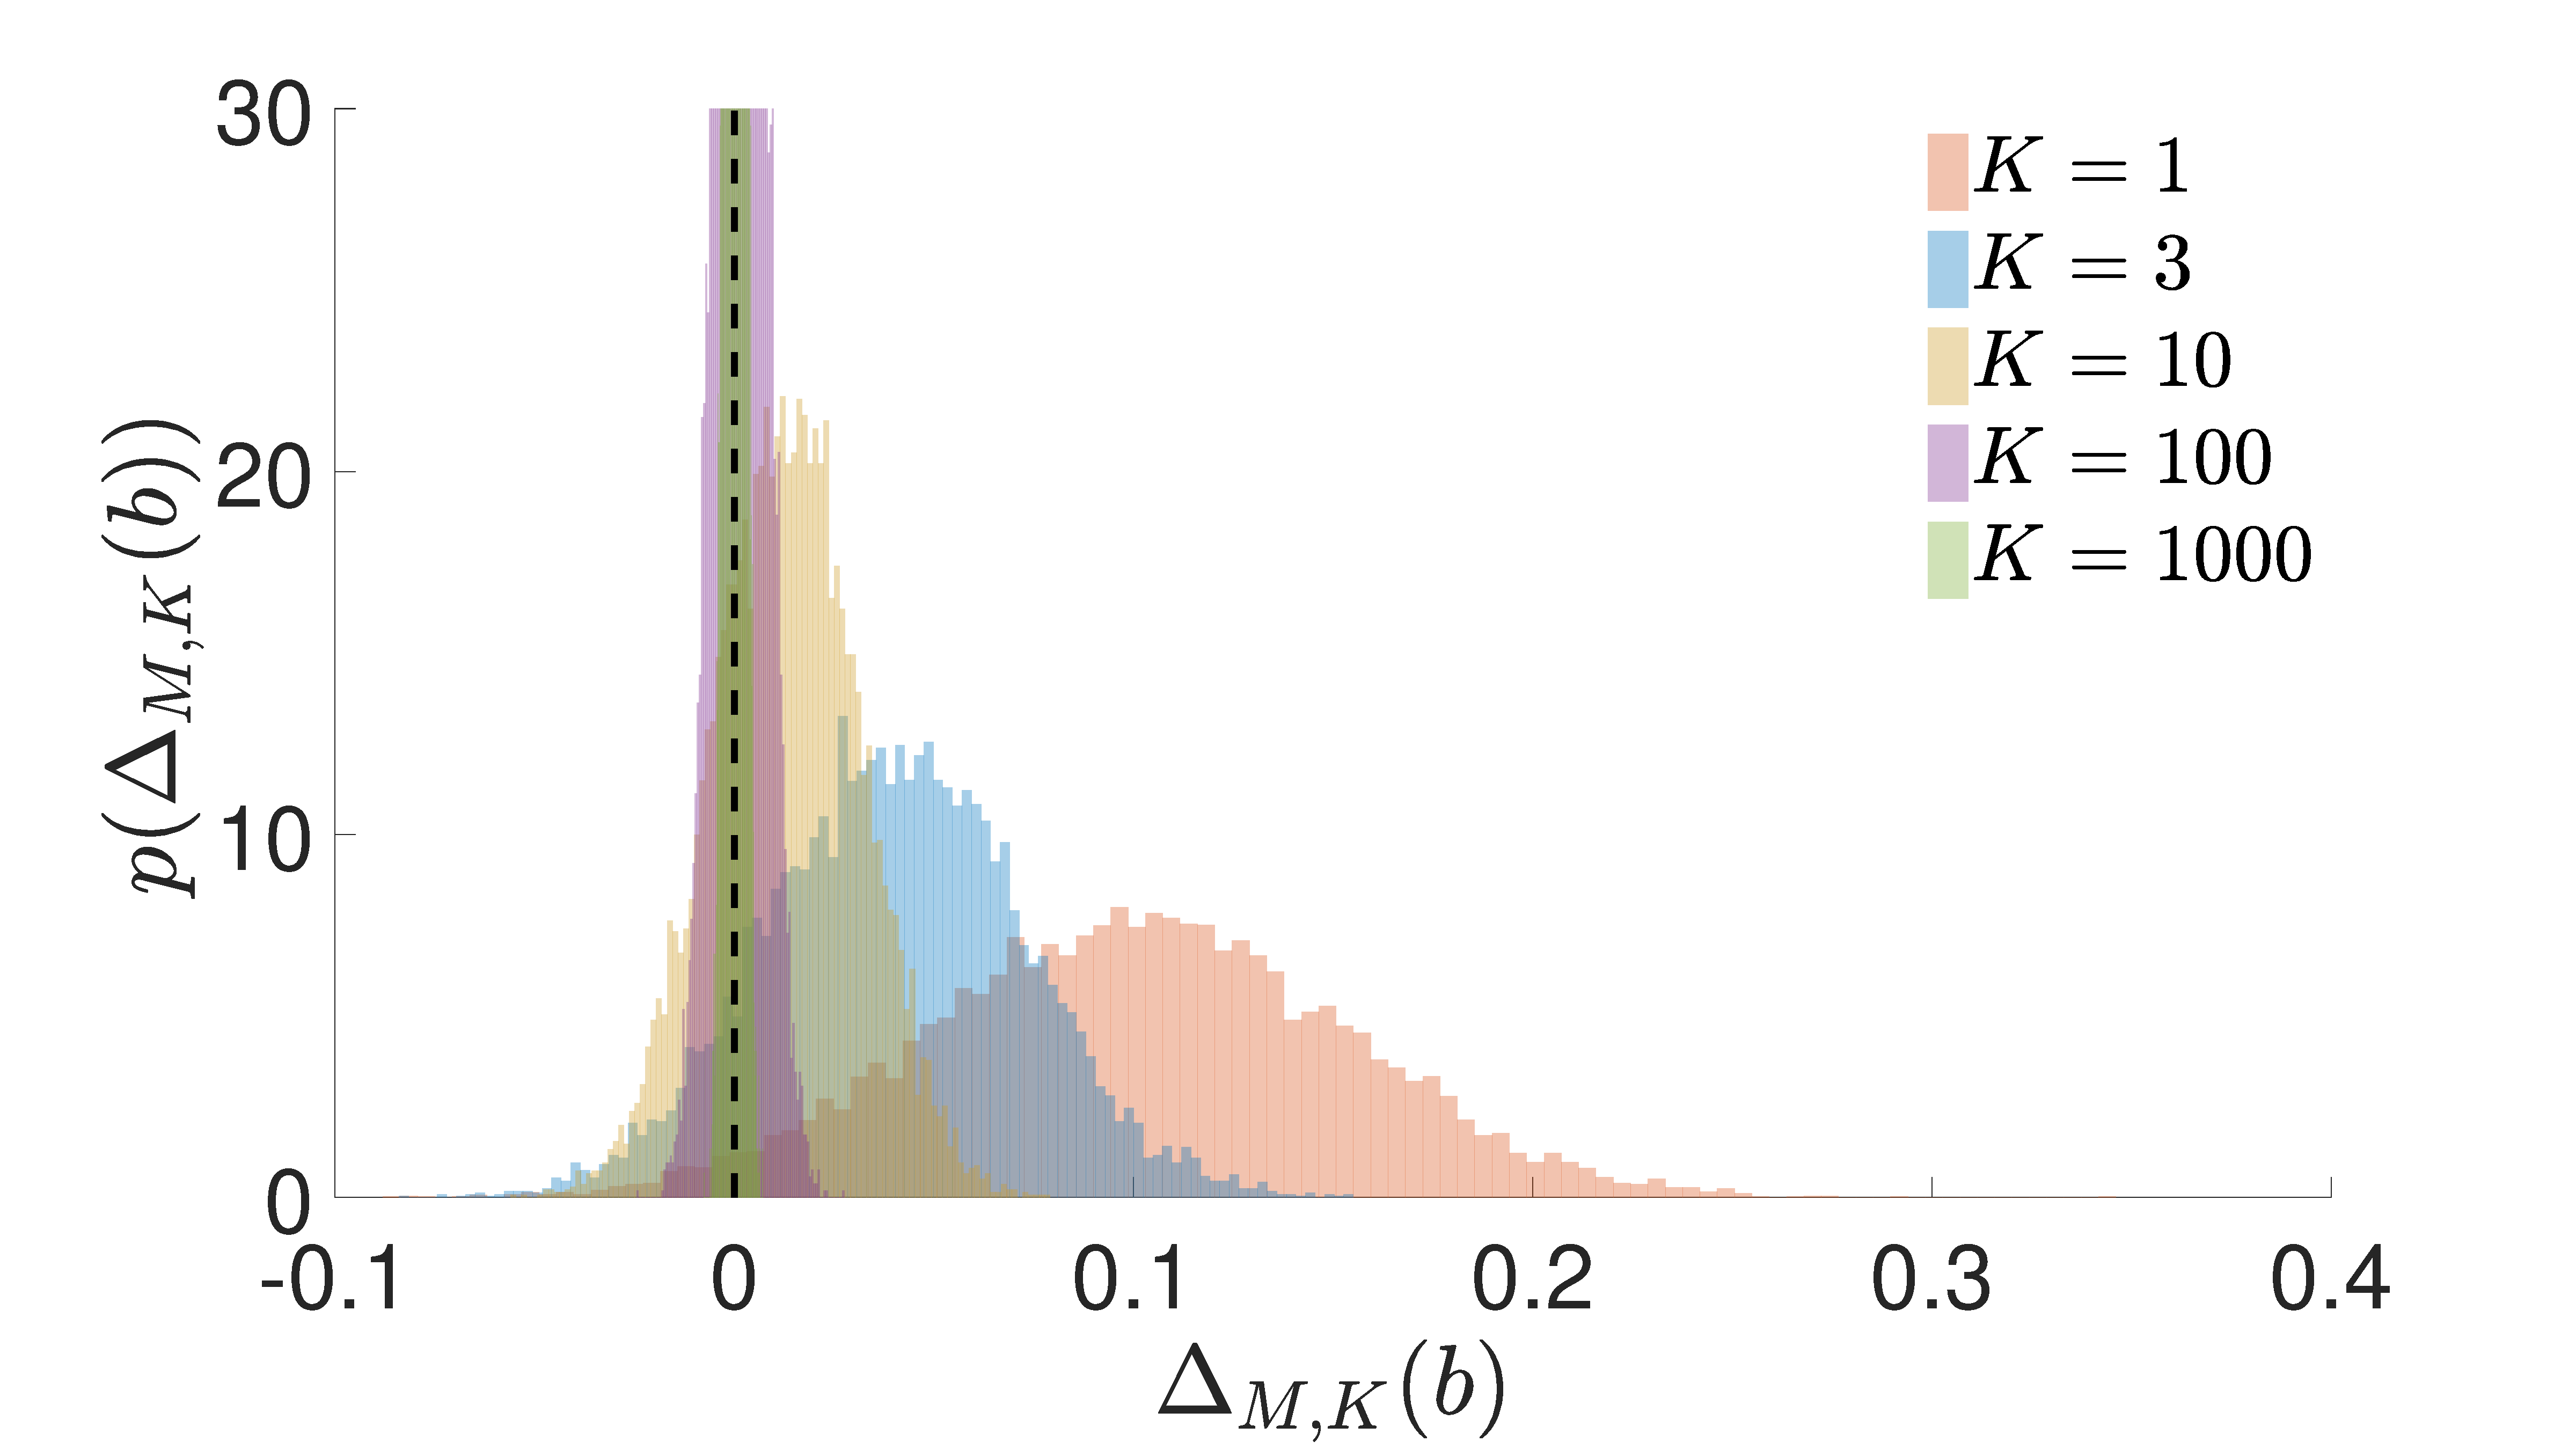
\includegraphics[width=\textwidth]{b_hist_IWAE}
%		\caption{\gls{IWAE} inference network gradient estimates \label{fig:snr/b_hist_iwae}}
%	\end{subfigure}
		\begin{subfigure}[b]{0.45\textwidth}
			\centering
			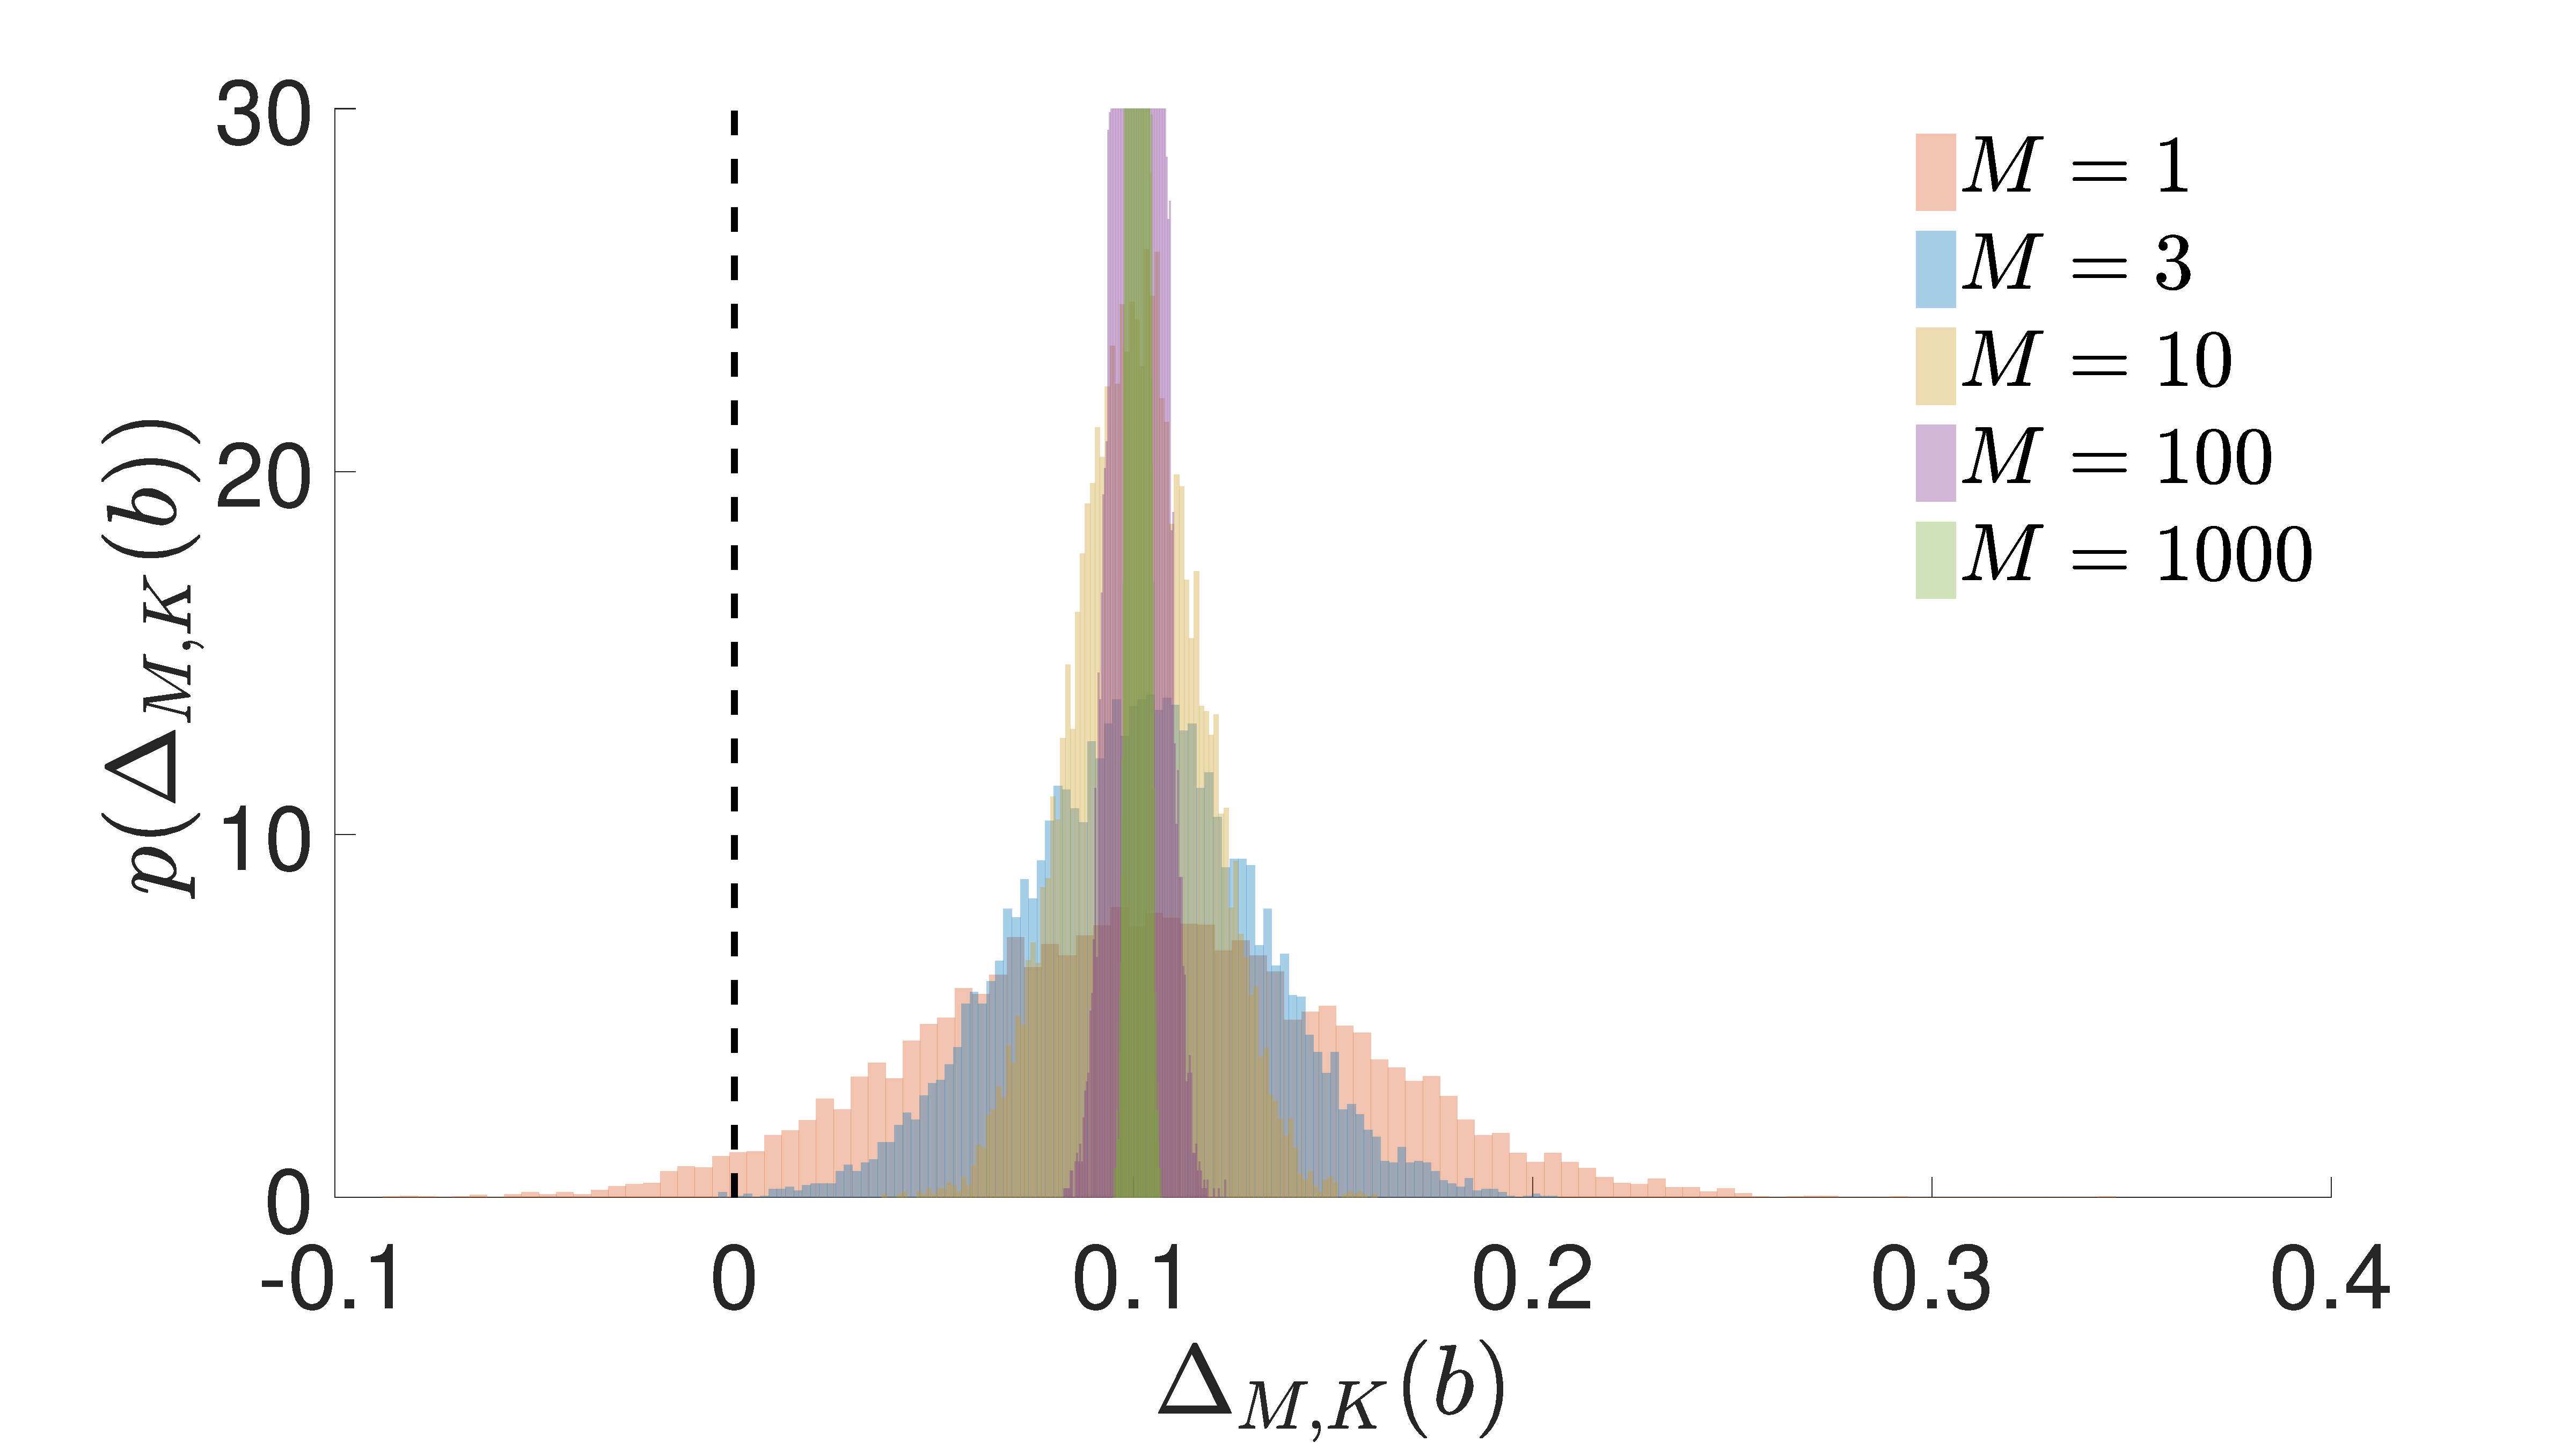
\includegraphics[width=\textwidth]{b_hist_VAE}
			\caption{\gls{VAE} inference network gradient estimates \label{fig:snr/b_hist_vae}}
		\end{subfigure} ~~~~~~~~~~
%	\begin{subfigure}[b]{0.49\textwidth}
%		\centering
%		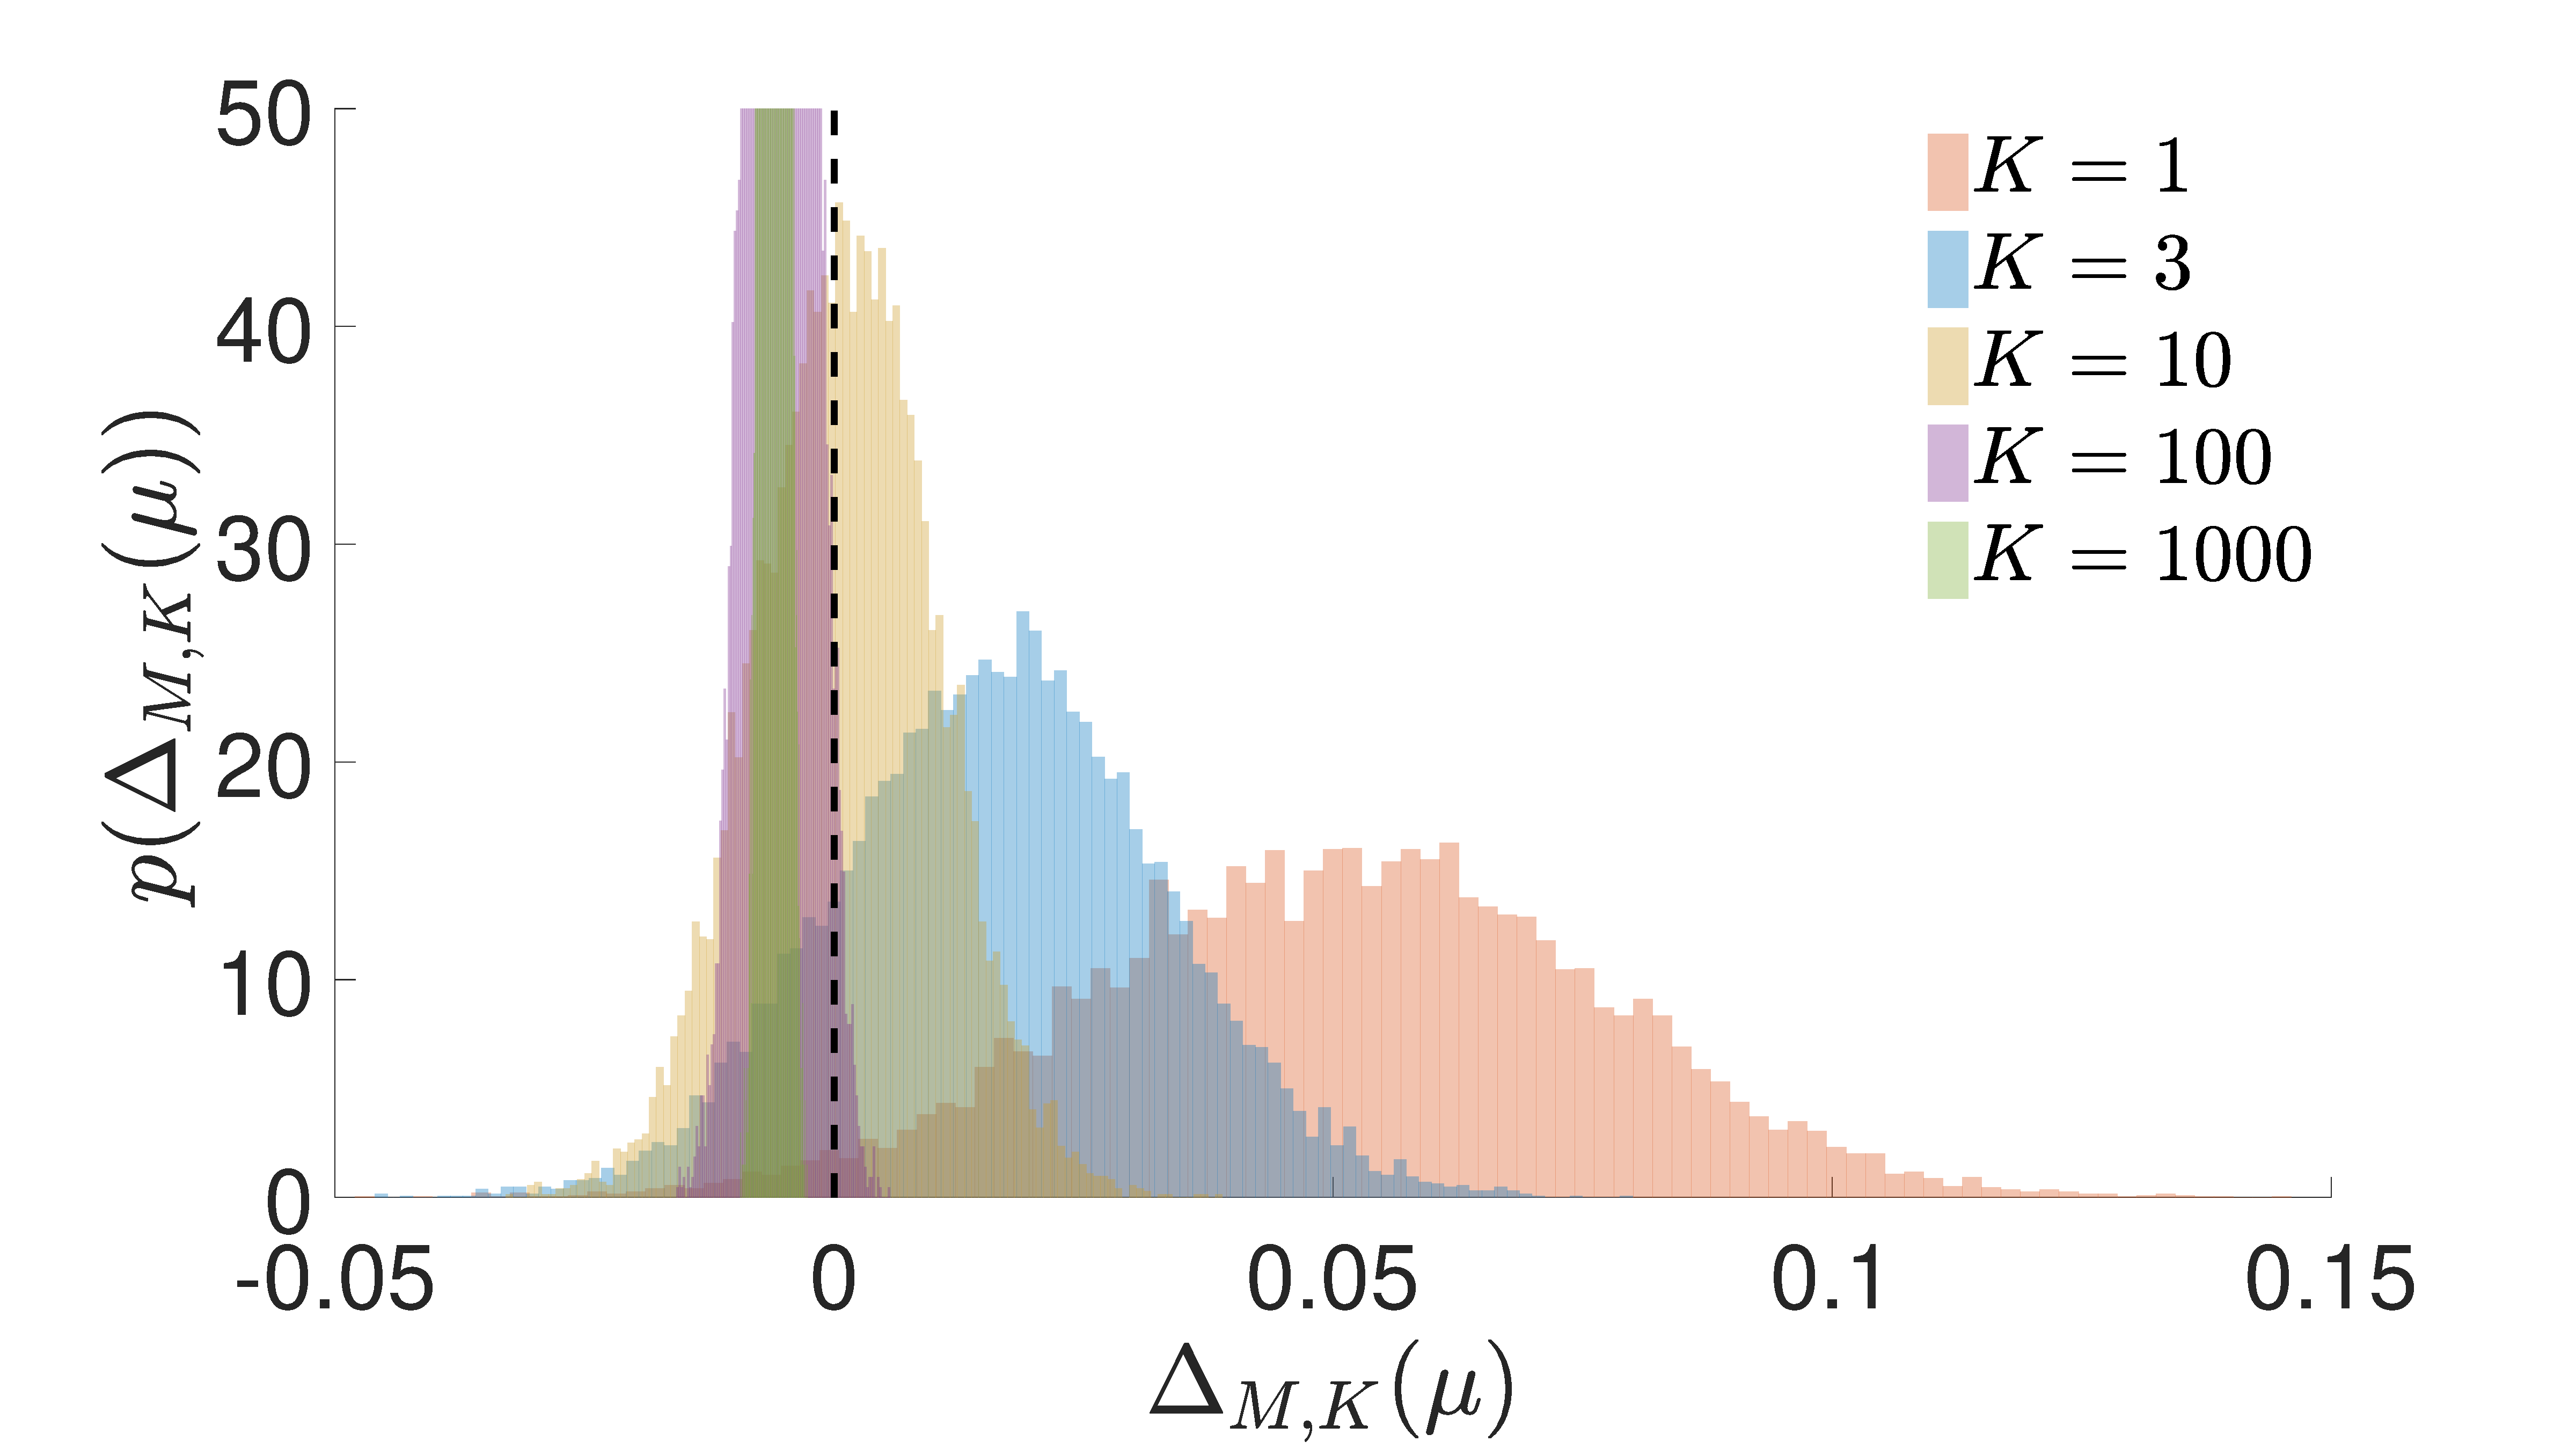
\includegraphics[width=\textwidth]{mu_hist_IWAE}
%		\caption{\gls{IWAE} generative network gradient estimates \label{fig:snr/mu_hist_iwae}}
%	\end{subfigure}
		\begin{subfigure}[b]{0.45\textwidth}
			\centering
			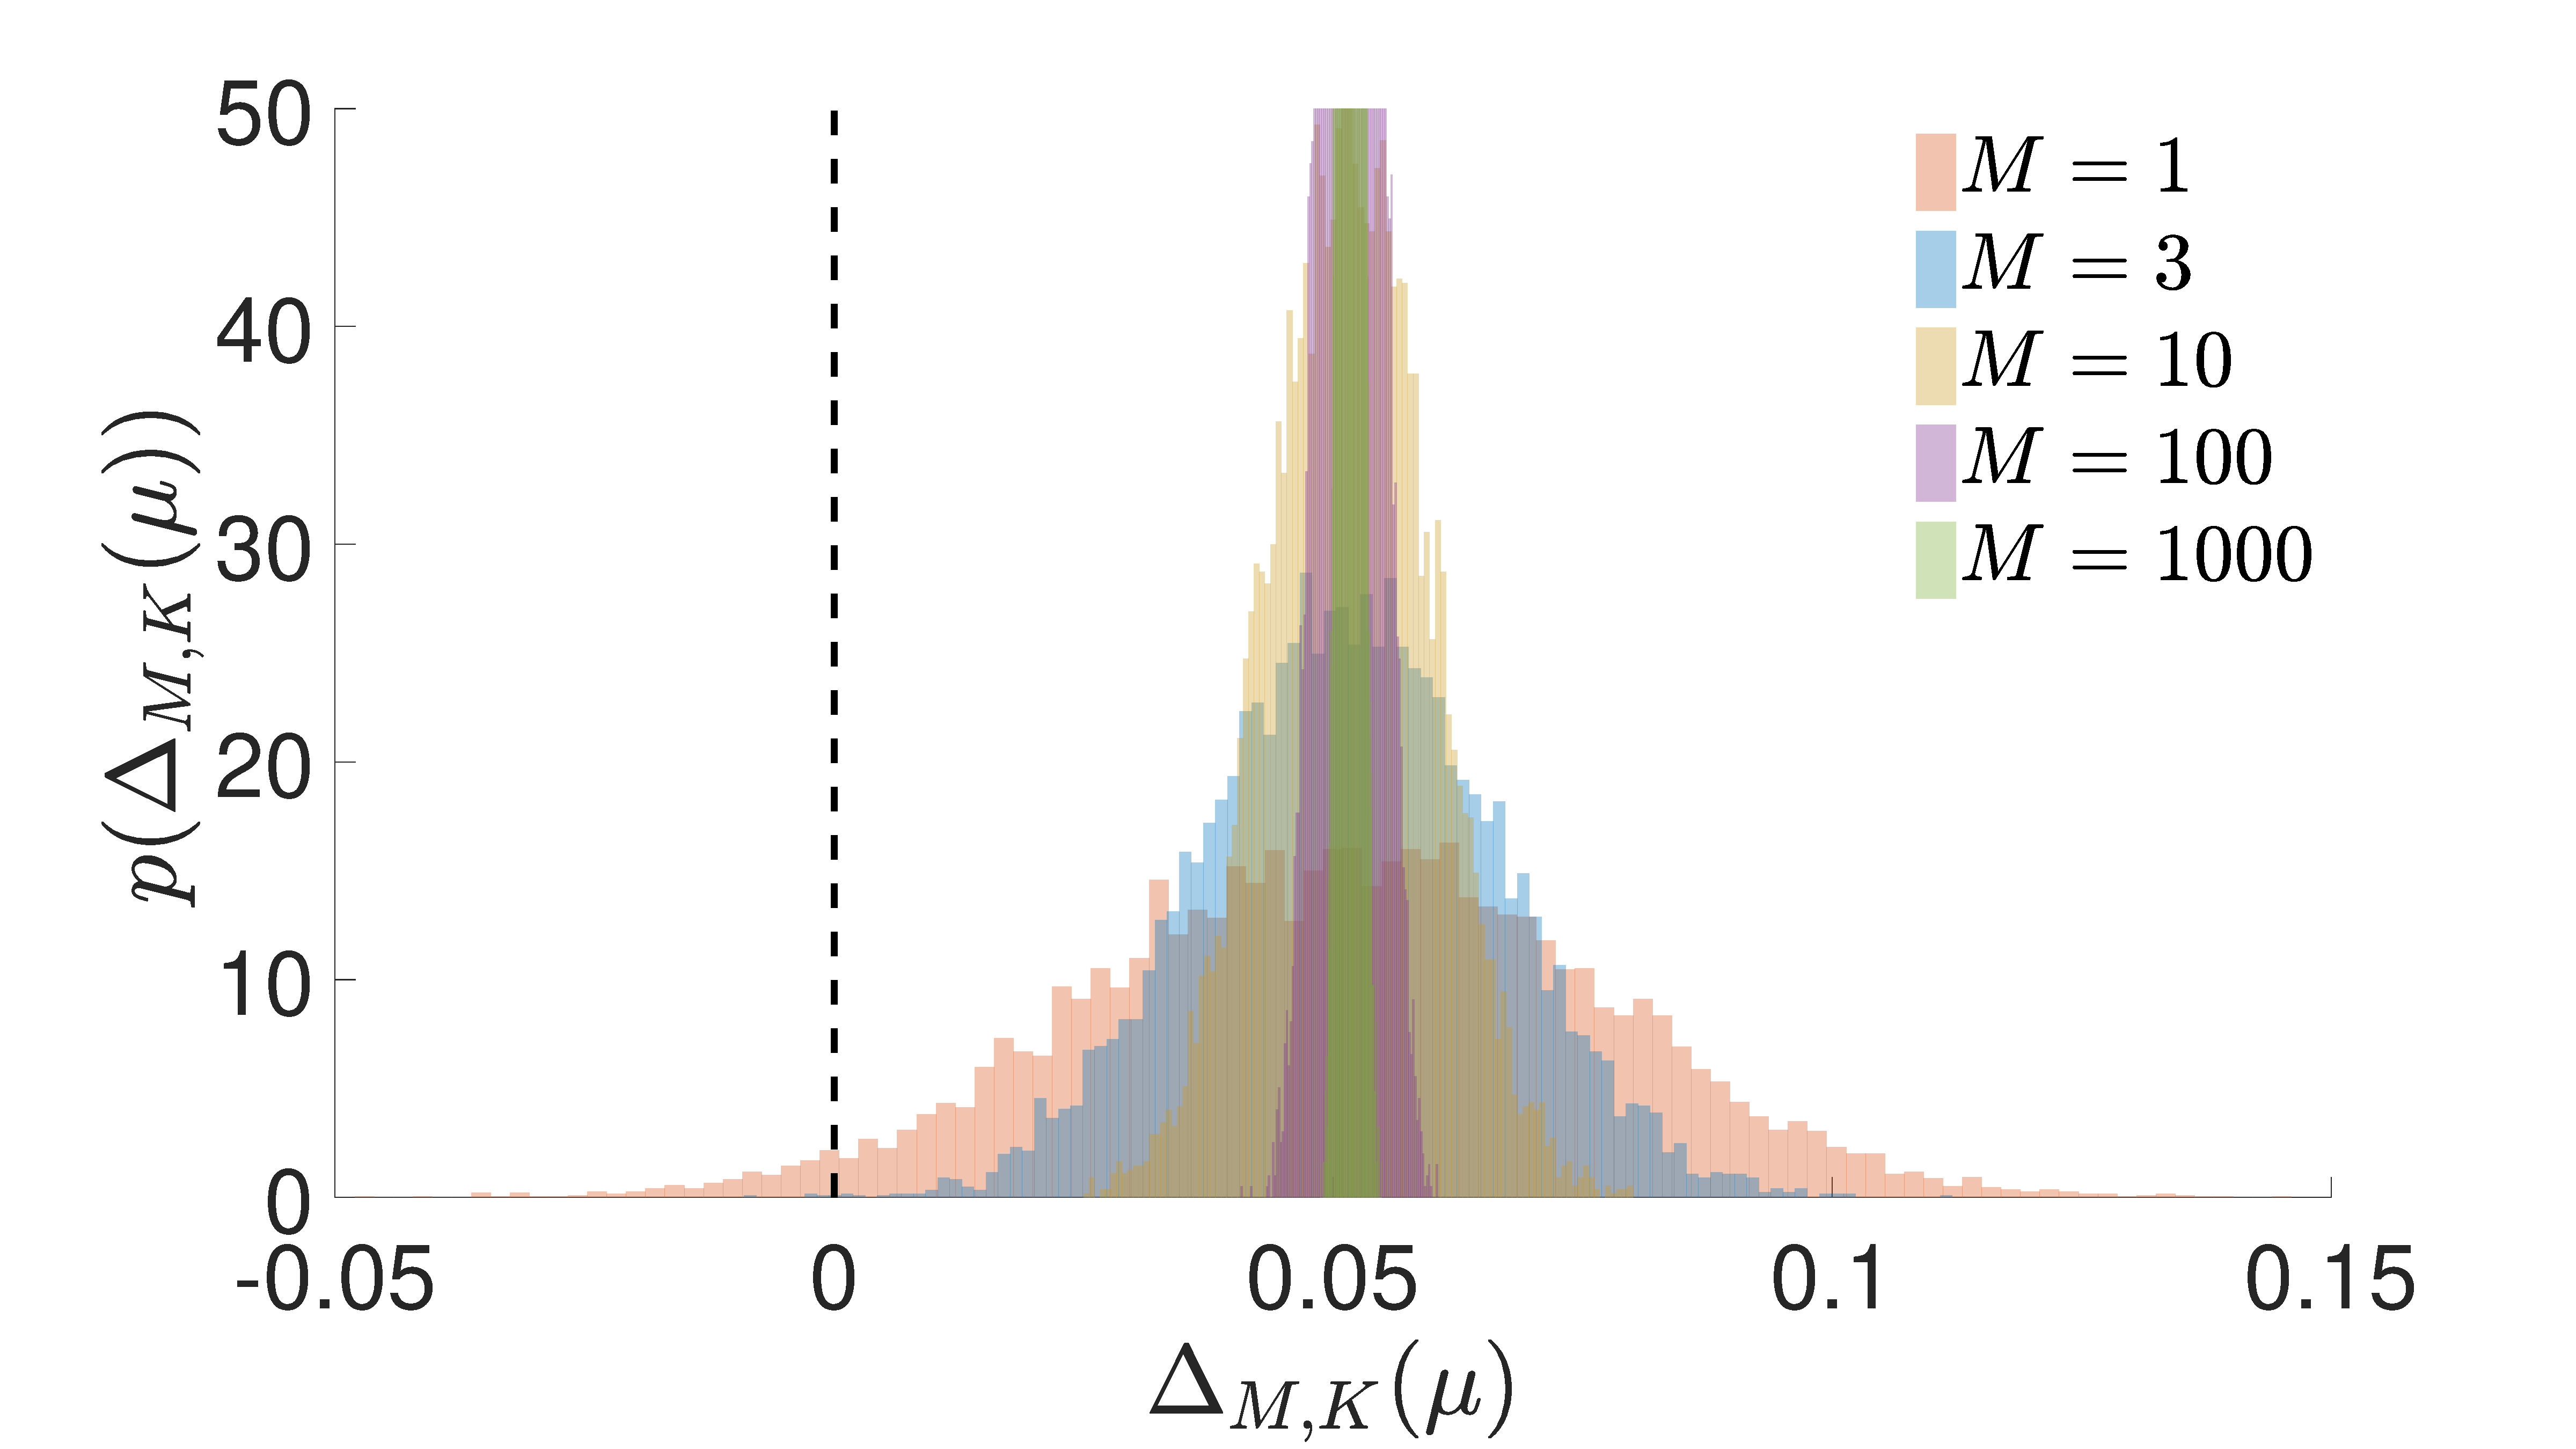
\includegraphics[width=\textwidth]{mu_hist_VAE}
			\caption{\gls{VAE} generative network gradient estimates \label{fig:snr/mu_hist_vae}}
		\end{subfigure}
	\caption{Histograms of gradient estimates $\Delta_{M,K}$ for the generative network and 
		the	inference network using the \gls{VAE} ($K=1$) objectives with different values of $M$. \vspace{-12pt}
		\label{fig:snr/hists-vae}}
\end{figure*}

\subsection{Convergence of RMSE for Generative Network}
\label{sec:app:rmse}

\begin{wrapfigure}{r}{0.5\textwidth}
	\centering
	\vspace{-15pt}
	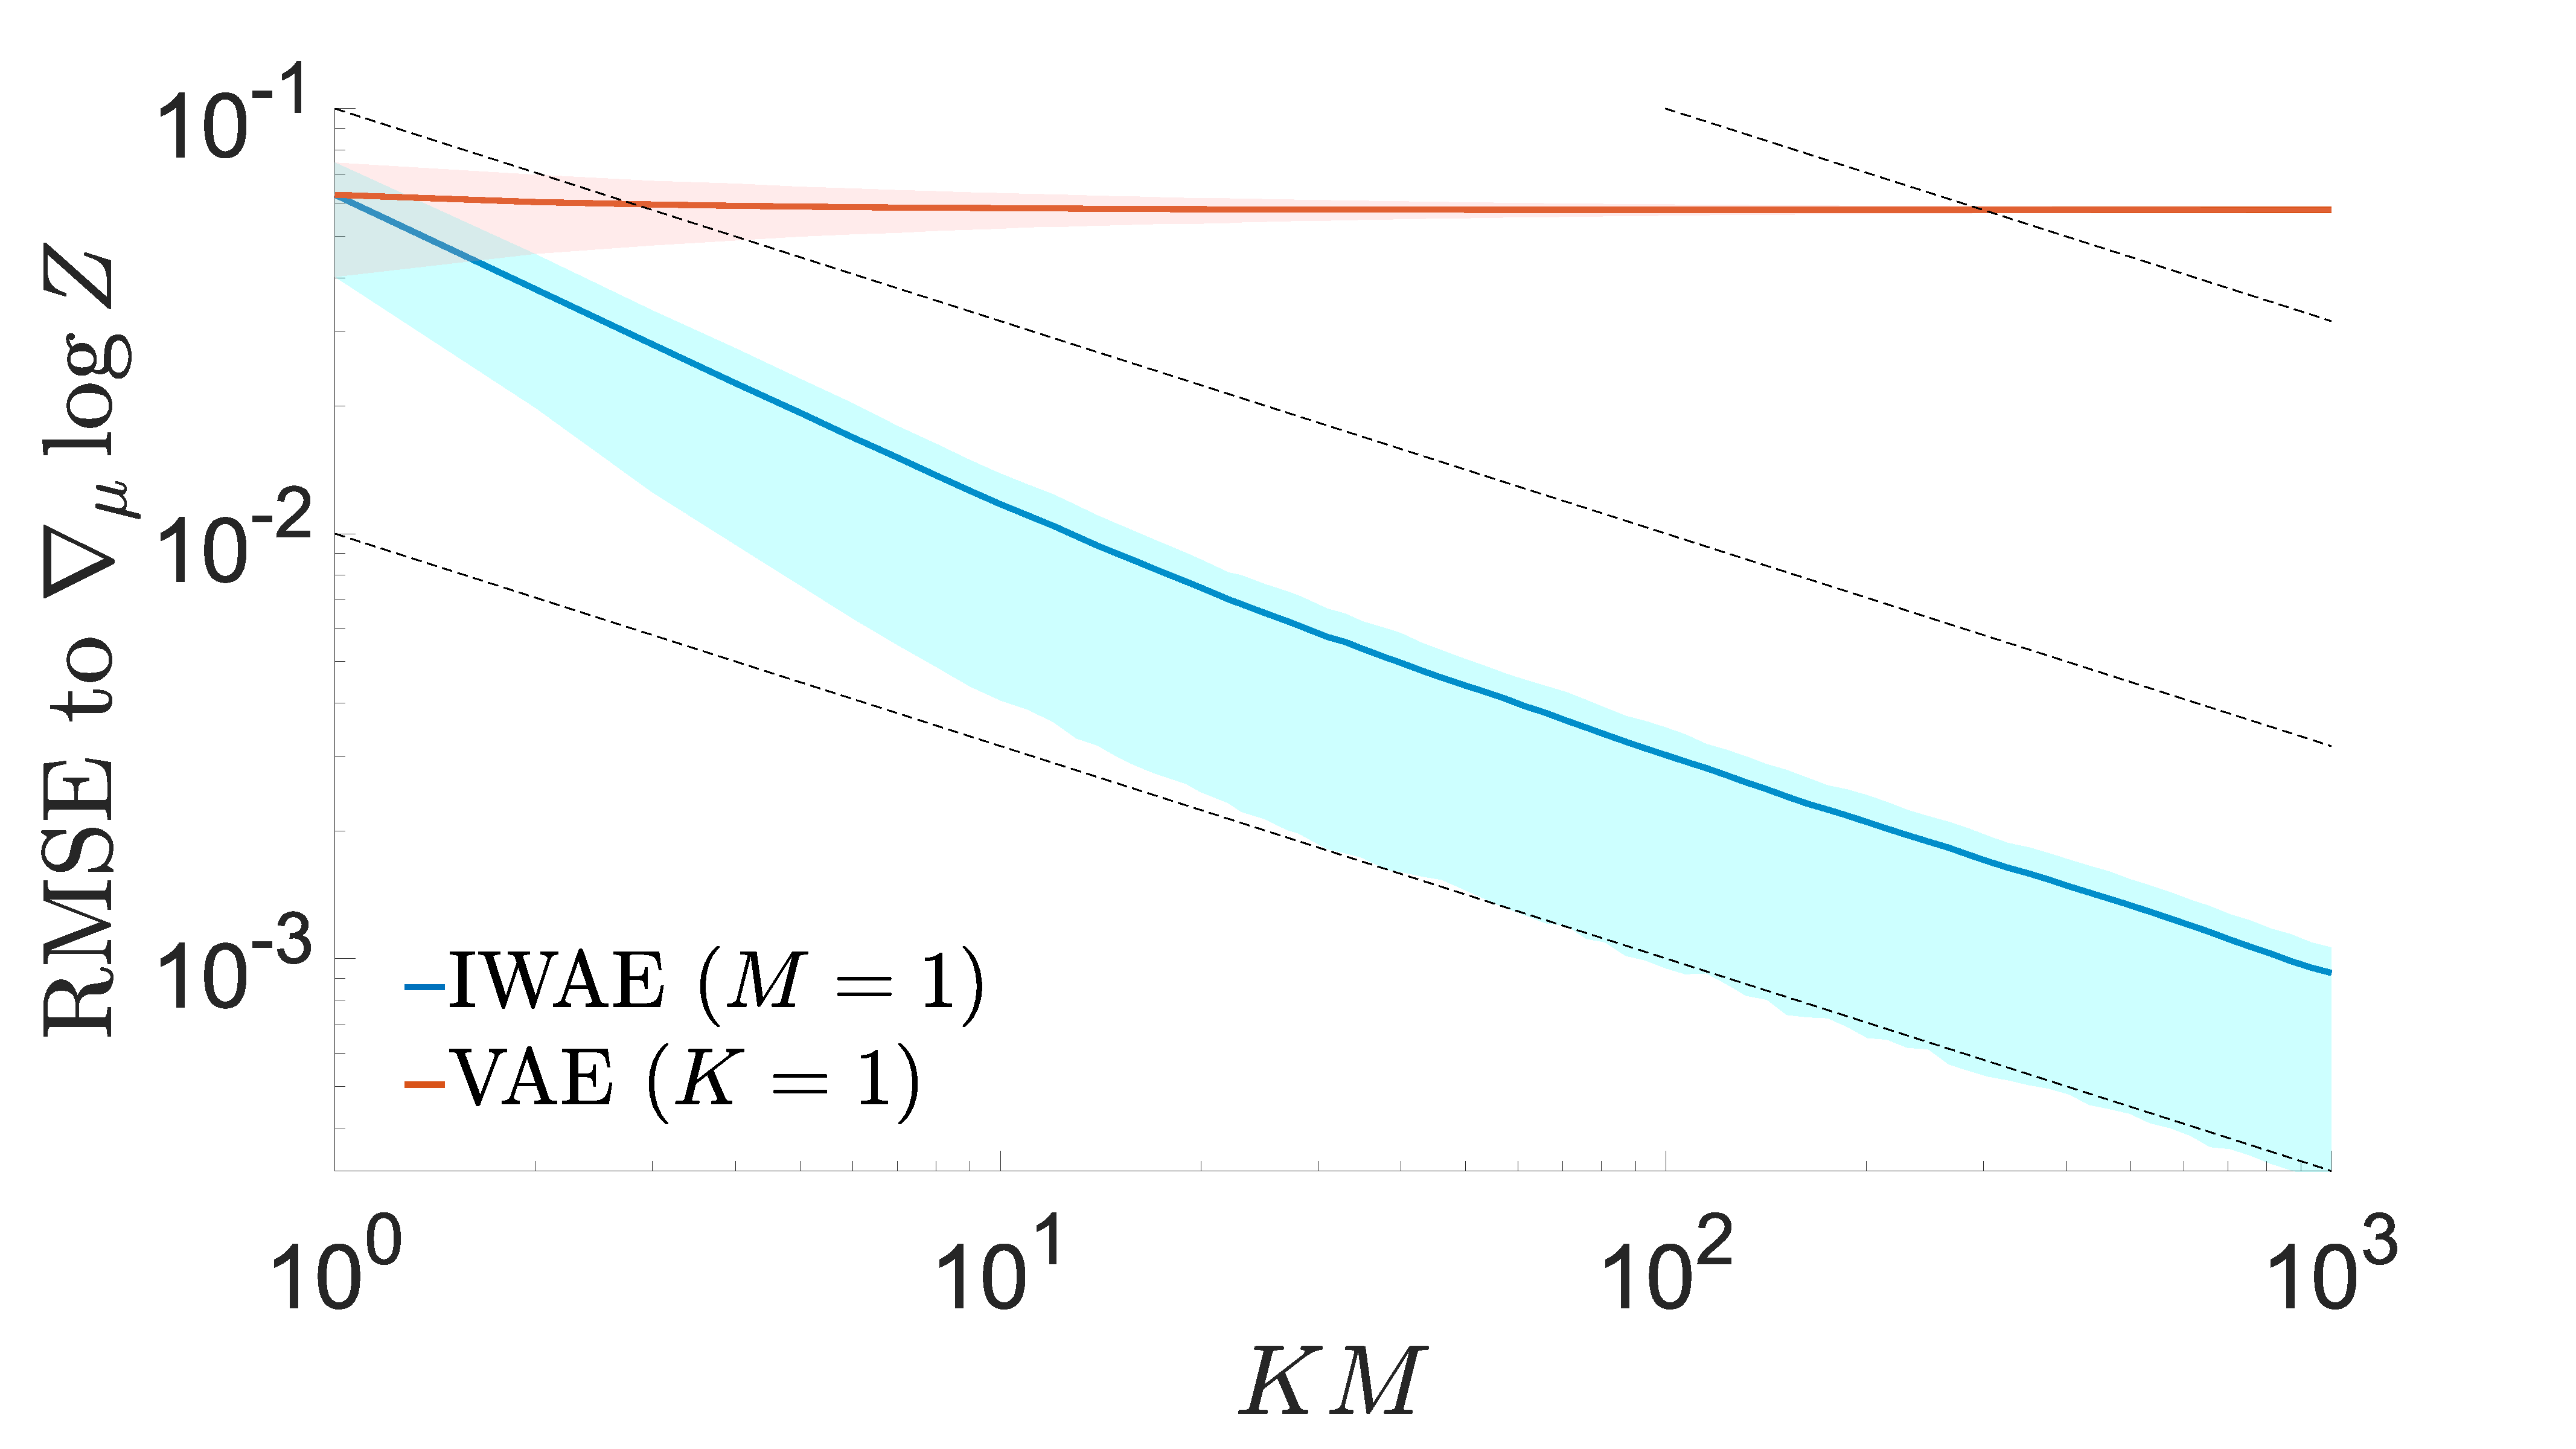
\includegraphics[width=0.47\textwidth]{mse_mu}
	\vspace{-10pt}
	\caption{RMSE in $\mu$ gradient estimate to $\nabla_{\mu} \log Z$ 
		\label{fig:snr/rmse}}
	\vspace{-8pt}
\end{wrapfigure} 
As explained in the main paper, the SNR is not an entirely appropriate metric for
the generative network -- a low SNR is still highly problematic, but a high SNR
does not indicate good performance.
It is thus perhaps better to measure
the quality of the gradient estimates for the generative network by looking at the \gls{RMSE}
to $\nabla_{\mu} \log Z$, i.e. $\sqrt{\E \left[\lVert\Delta_{M,K}-\nabla_{\mu} \log Z\rVert_2^2\right]}$.
The convergence of this \gls{RMSE}  is shown in
Figure~\ref{fig:snr/rmse} where the solid lines are the \gls{RMSE} estimates using $10^4$ runs 
and the shaded regions
show the interquartile range of the individual estimates. We see that increasing 
$M$ in the \gls{VAE} reduces the variance
of the estimates but has negligible effect on the \gls{RMSE} due to the fixed bias.  On the
other hand,
we see that increasing $K$ leads to a monotonic improvement, initially improving
at a rate $O(1/K)$ (because the bias is the dominating term in this region),
before settling to the standard Monte Carlo convergence rate of $O(1/\sqrt{K})$
(shown by the dashed lines).

\subsection{Experimental Results for High Variance Regime}
\label{sec:hv}

\vspace{-4pt}

We now present empirical results for a case where our weights are higher variance. Instead
of choosing a point close to the optimum by offsetting parameters with a standard deviation of $0.01$, 
we instead offset using a standard deviation of $0.5$.  We further increased the proposal covariance to $I$
to make it more diffuse.  This is now a scenario where the model is far from its optimum and the proposal
is a very poor match for the model, giving very high variance weights.


We see that the behavior is the
same for variation in $M$, but somewhat distinct for variation in $K$.  
In particular, the \gls{SNR} and \textsc{dsnr} only decrease slowly with $K$ for the inference network, while increasing $K$ no longer has much benefit for the \gls{SNR} of the
inference network.
%Increasing $K$ now also has a remarkably similar impact on the \gls{SNR} and \textsc{dsnr} of
%the gradients of the generative network as on the
%inference network.  
It is clear that, for this
setup, the problem is very far from the asymptotic regime in $K$ such that our theoretical results no
longer directly apply.  Nonetheless, the high-level effect observed is still that the \gls{SNR} of 
the inference
network deteriorates, albeit slowly, as $K$ increases.

\begin{figure}[h]
	\centering
	\begin{subfigure}[b]{0.45\textwidth}
		\centering
		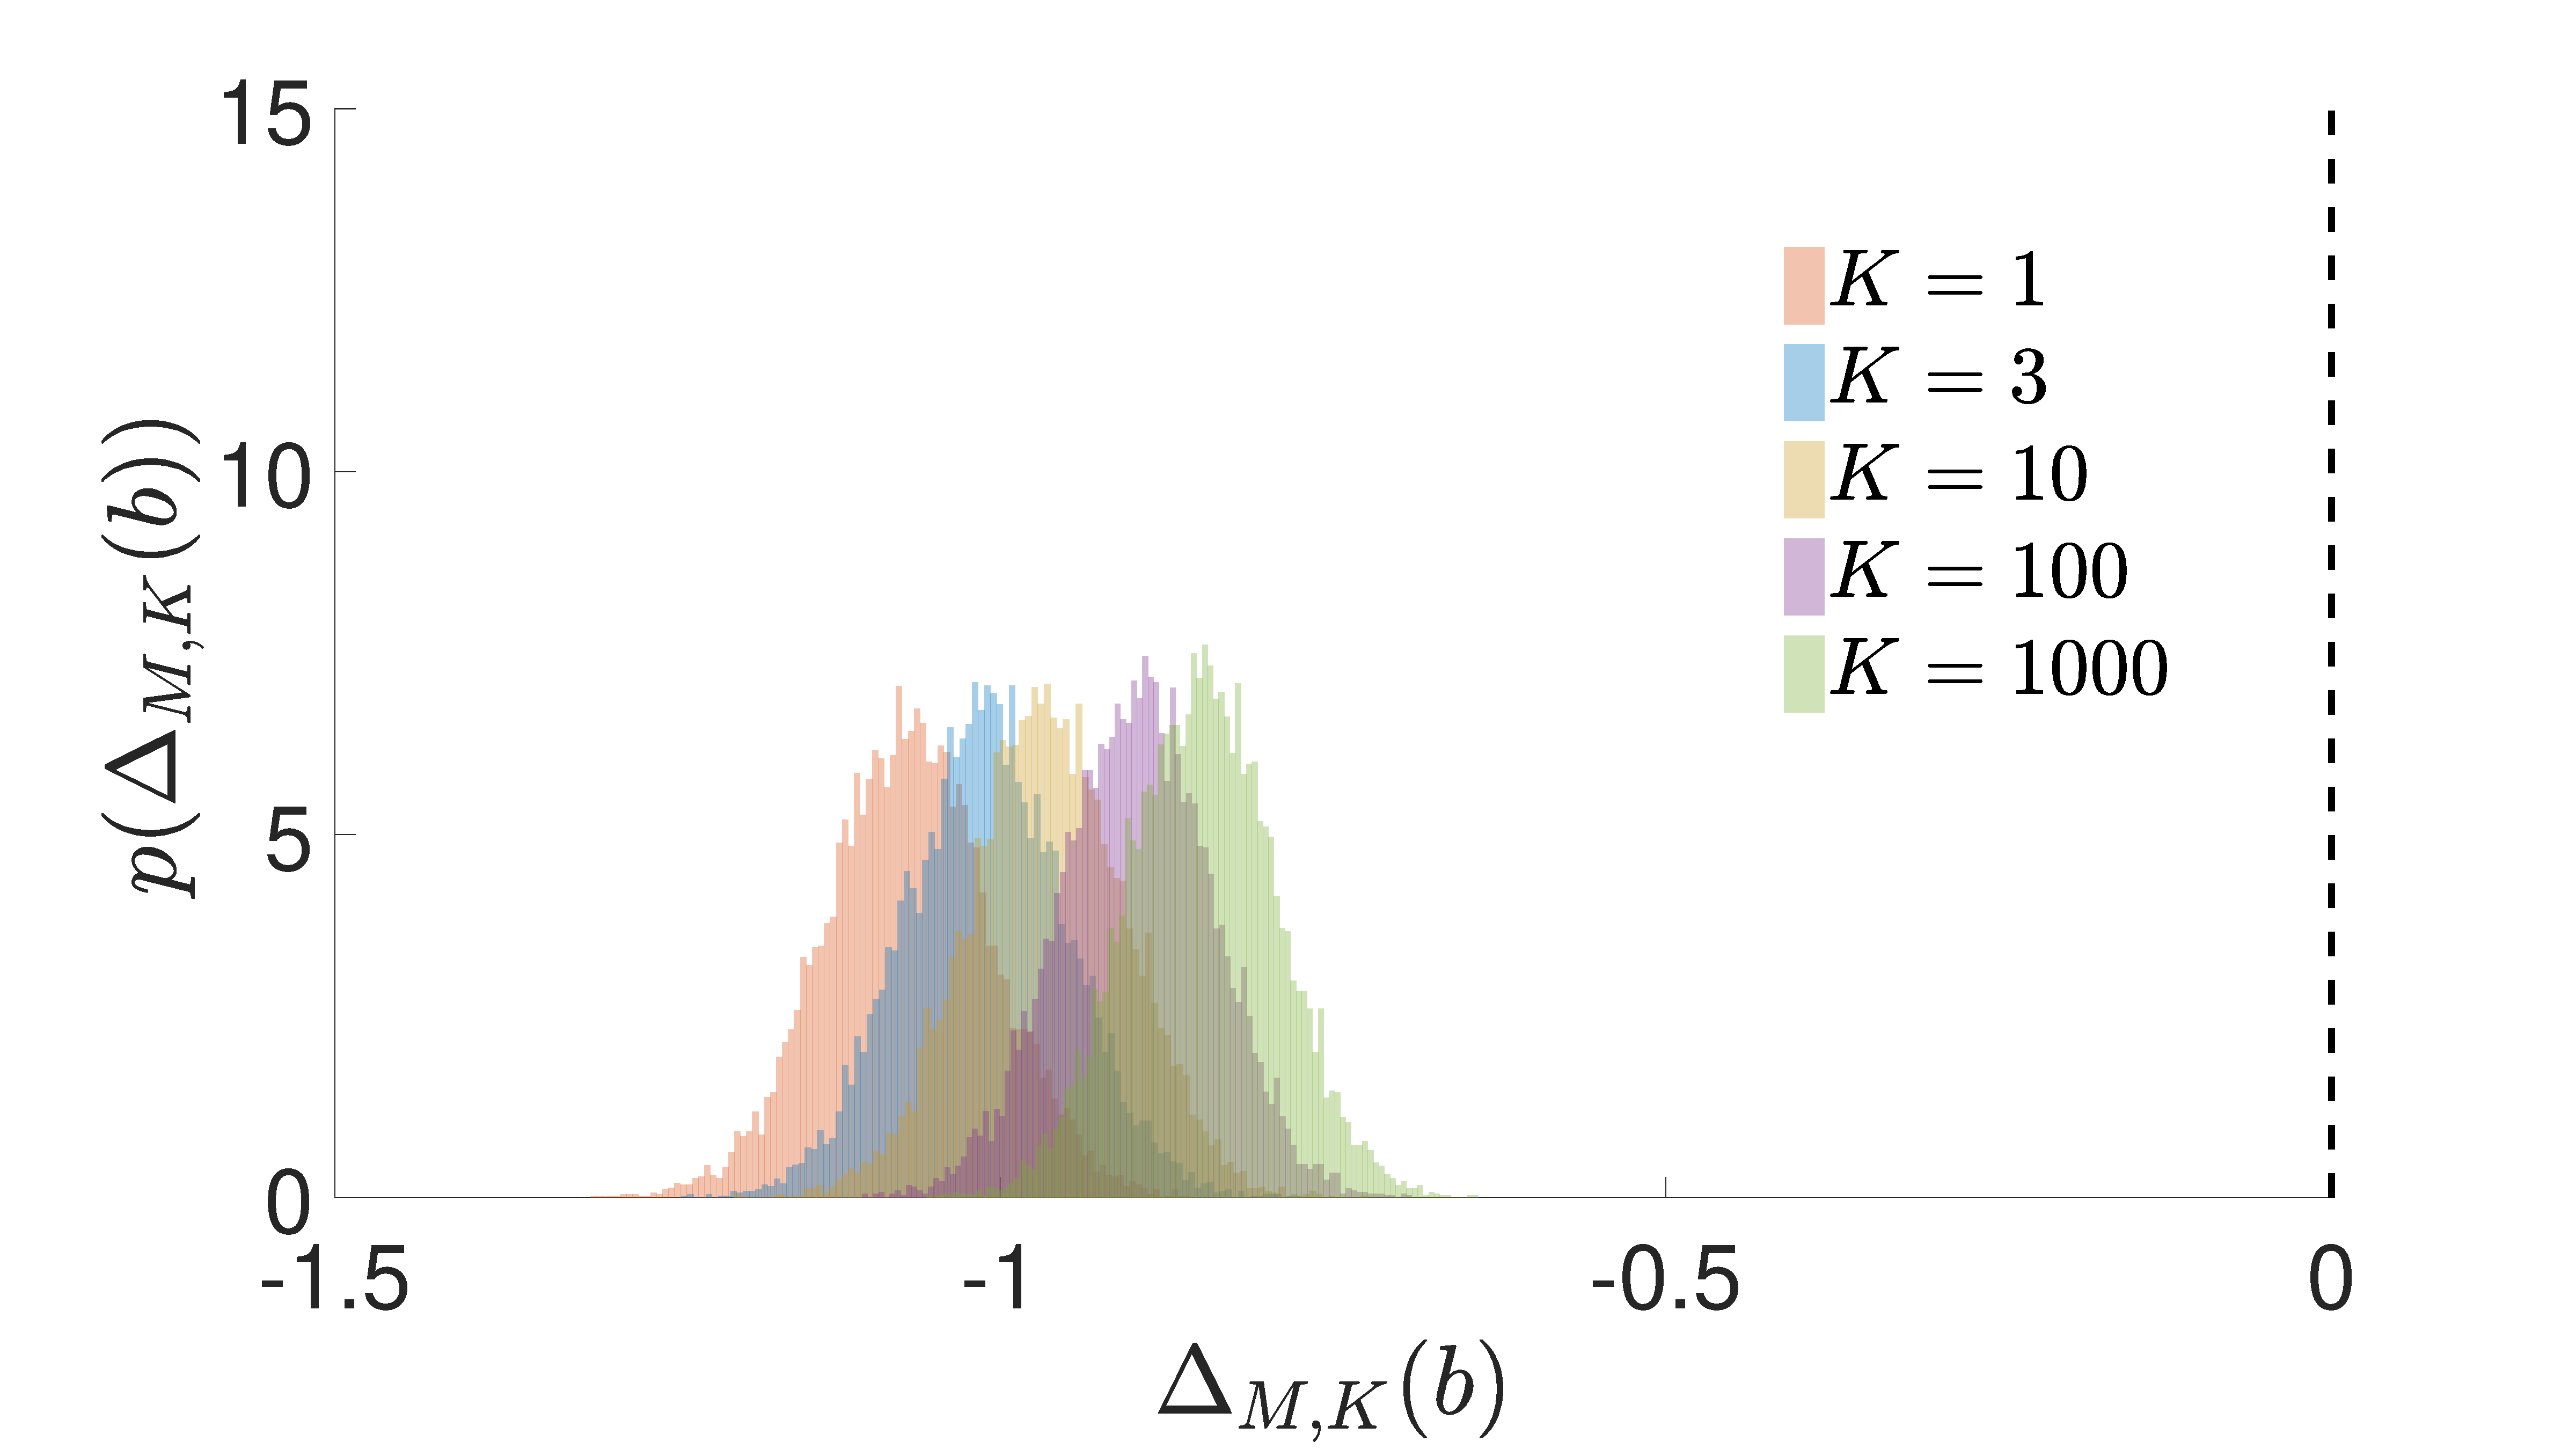
\includegraphics[width=\textwidth]{hv_b_hist_IWAE}
		\caption{\gls{IWAE} inference network gradient estimates \label{fig:hv/b_hist_iwae}}
	\end{subfigure} ~~~~~~~~~~
	\begin{subfigure}[b]{0.45\textwidth}
		\centering
		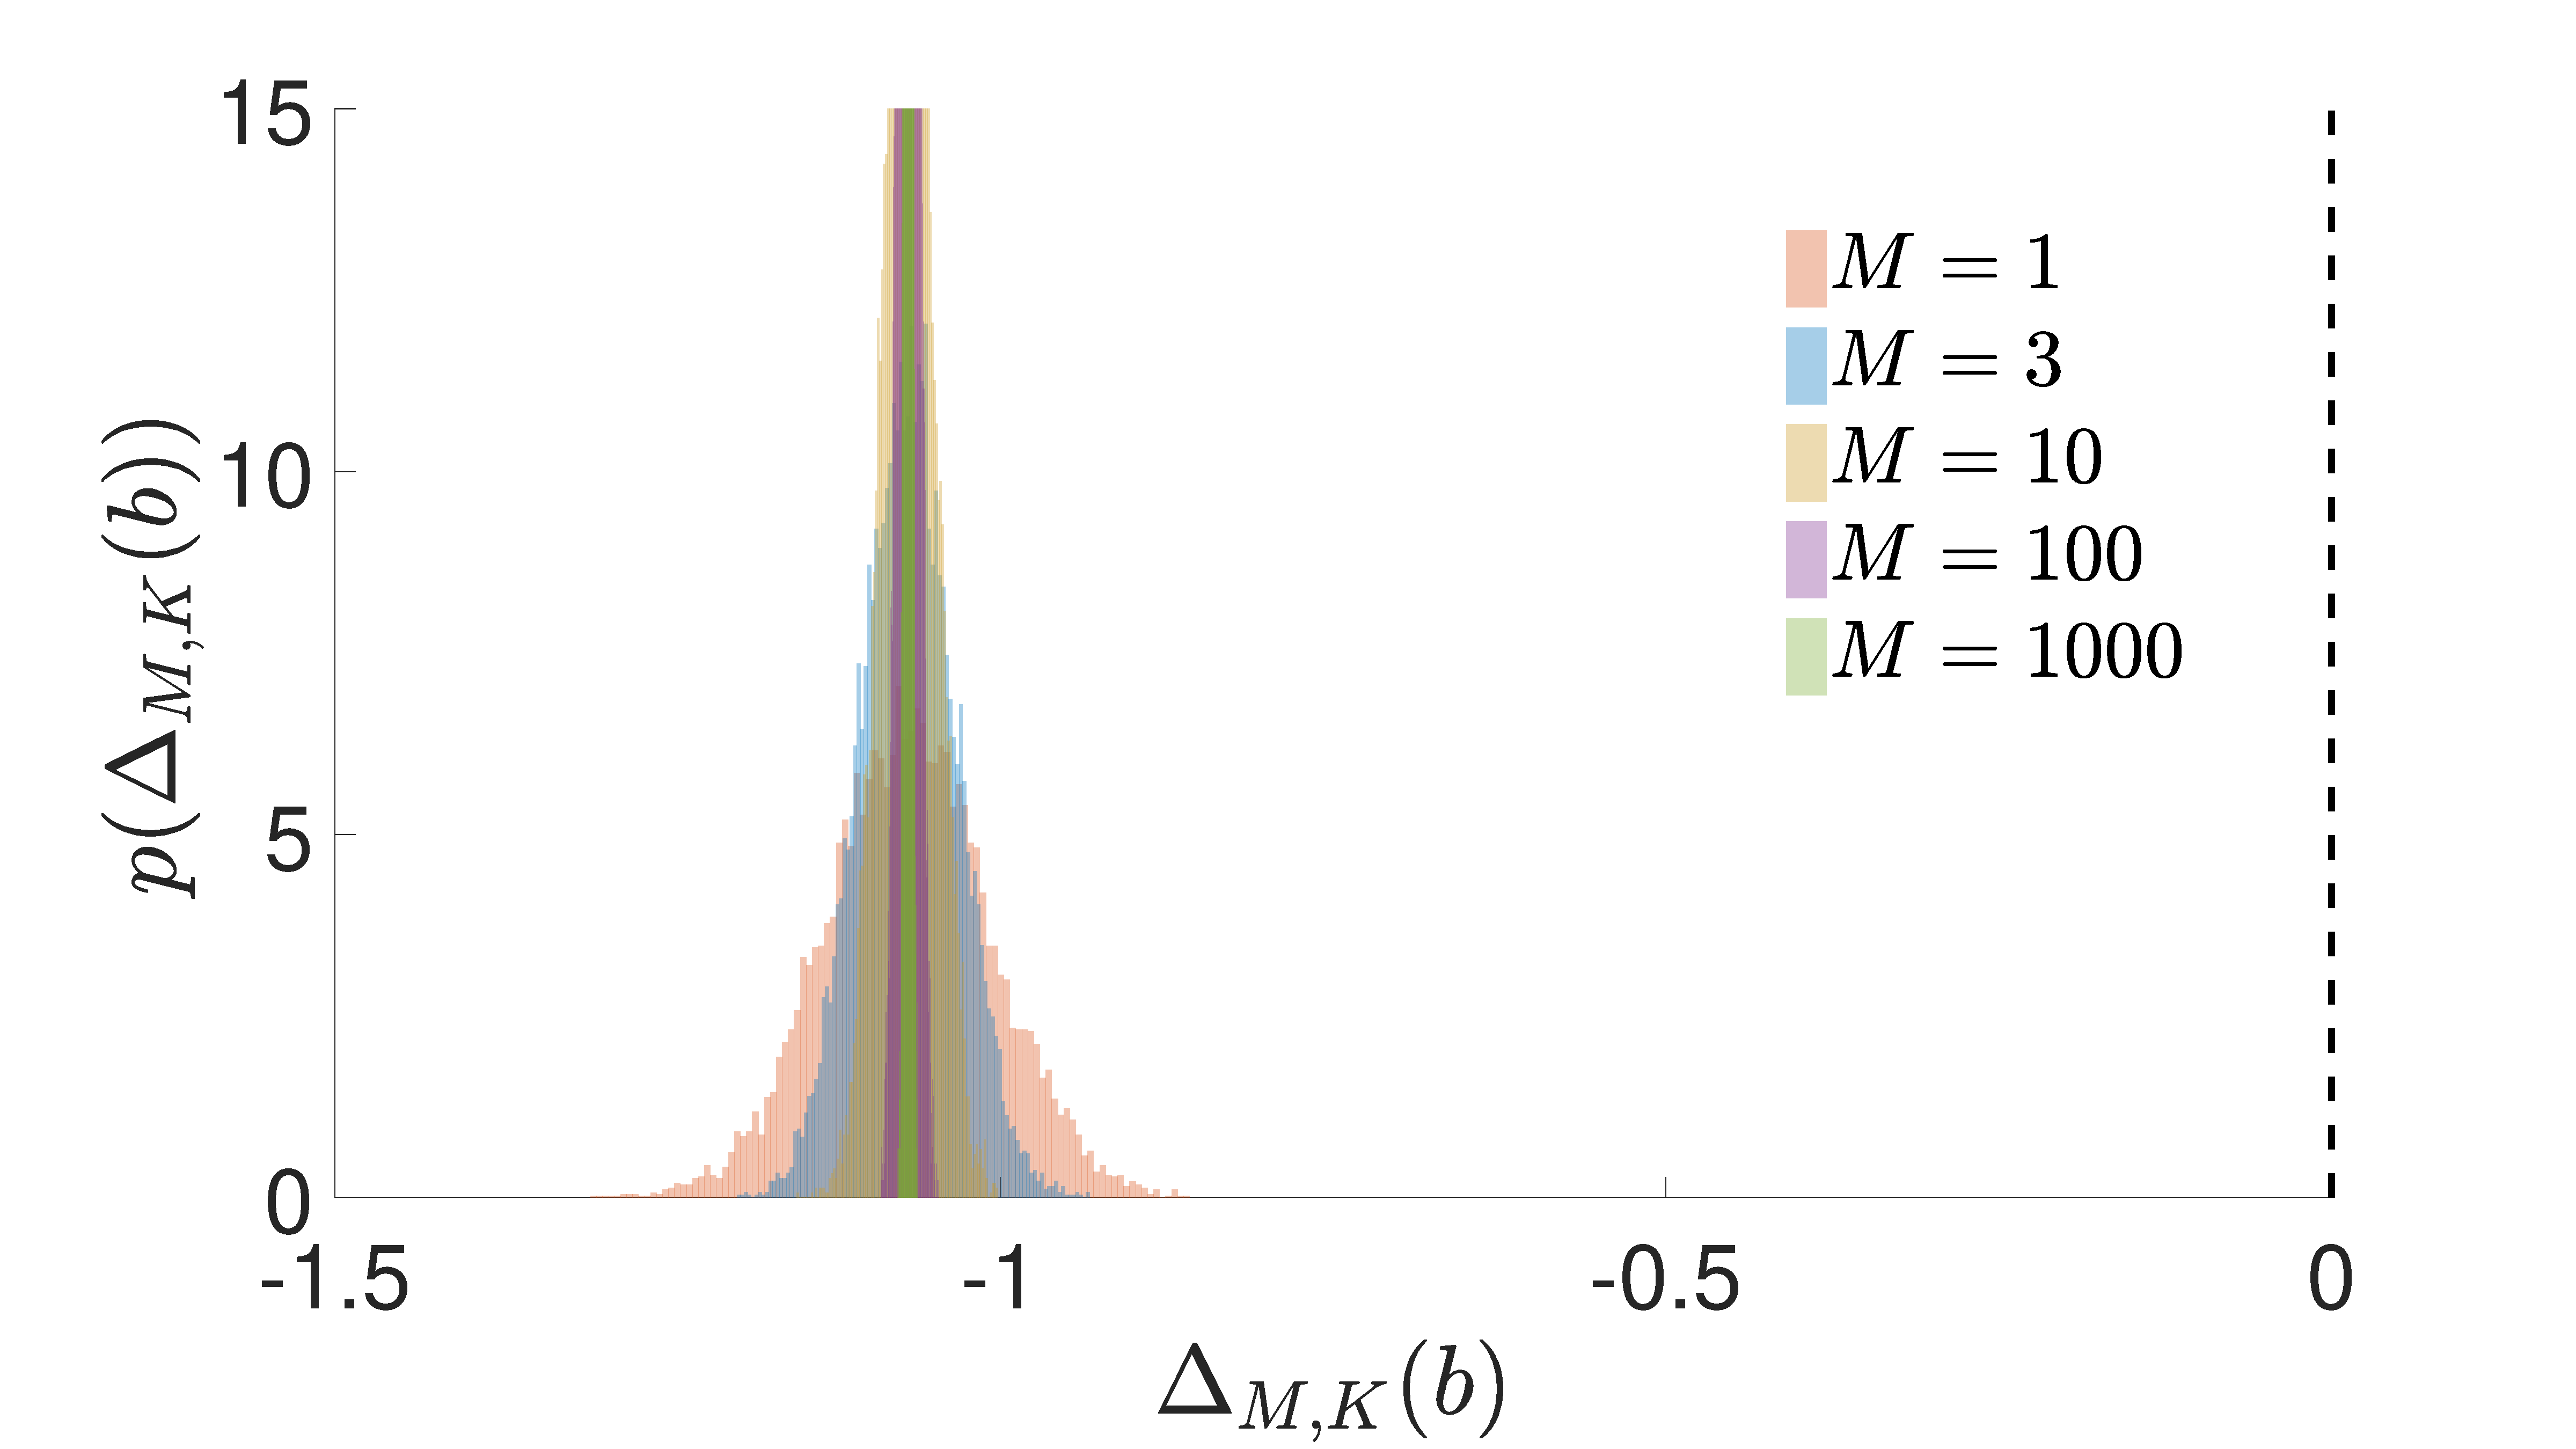
\includegraphics[width=\textwidth]{hv_b_hist_VAE}
		\caption{\gls{VAE} inference network gradient estimates \label{fig:hv/b_hist_vae}}
	\end{subfigure}\\
	\begin{subfigure}[b]{0.45\textwidth}
		\centering
		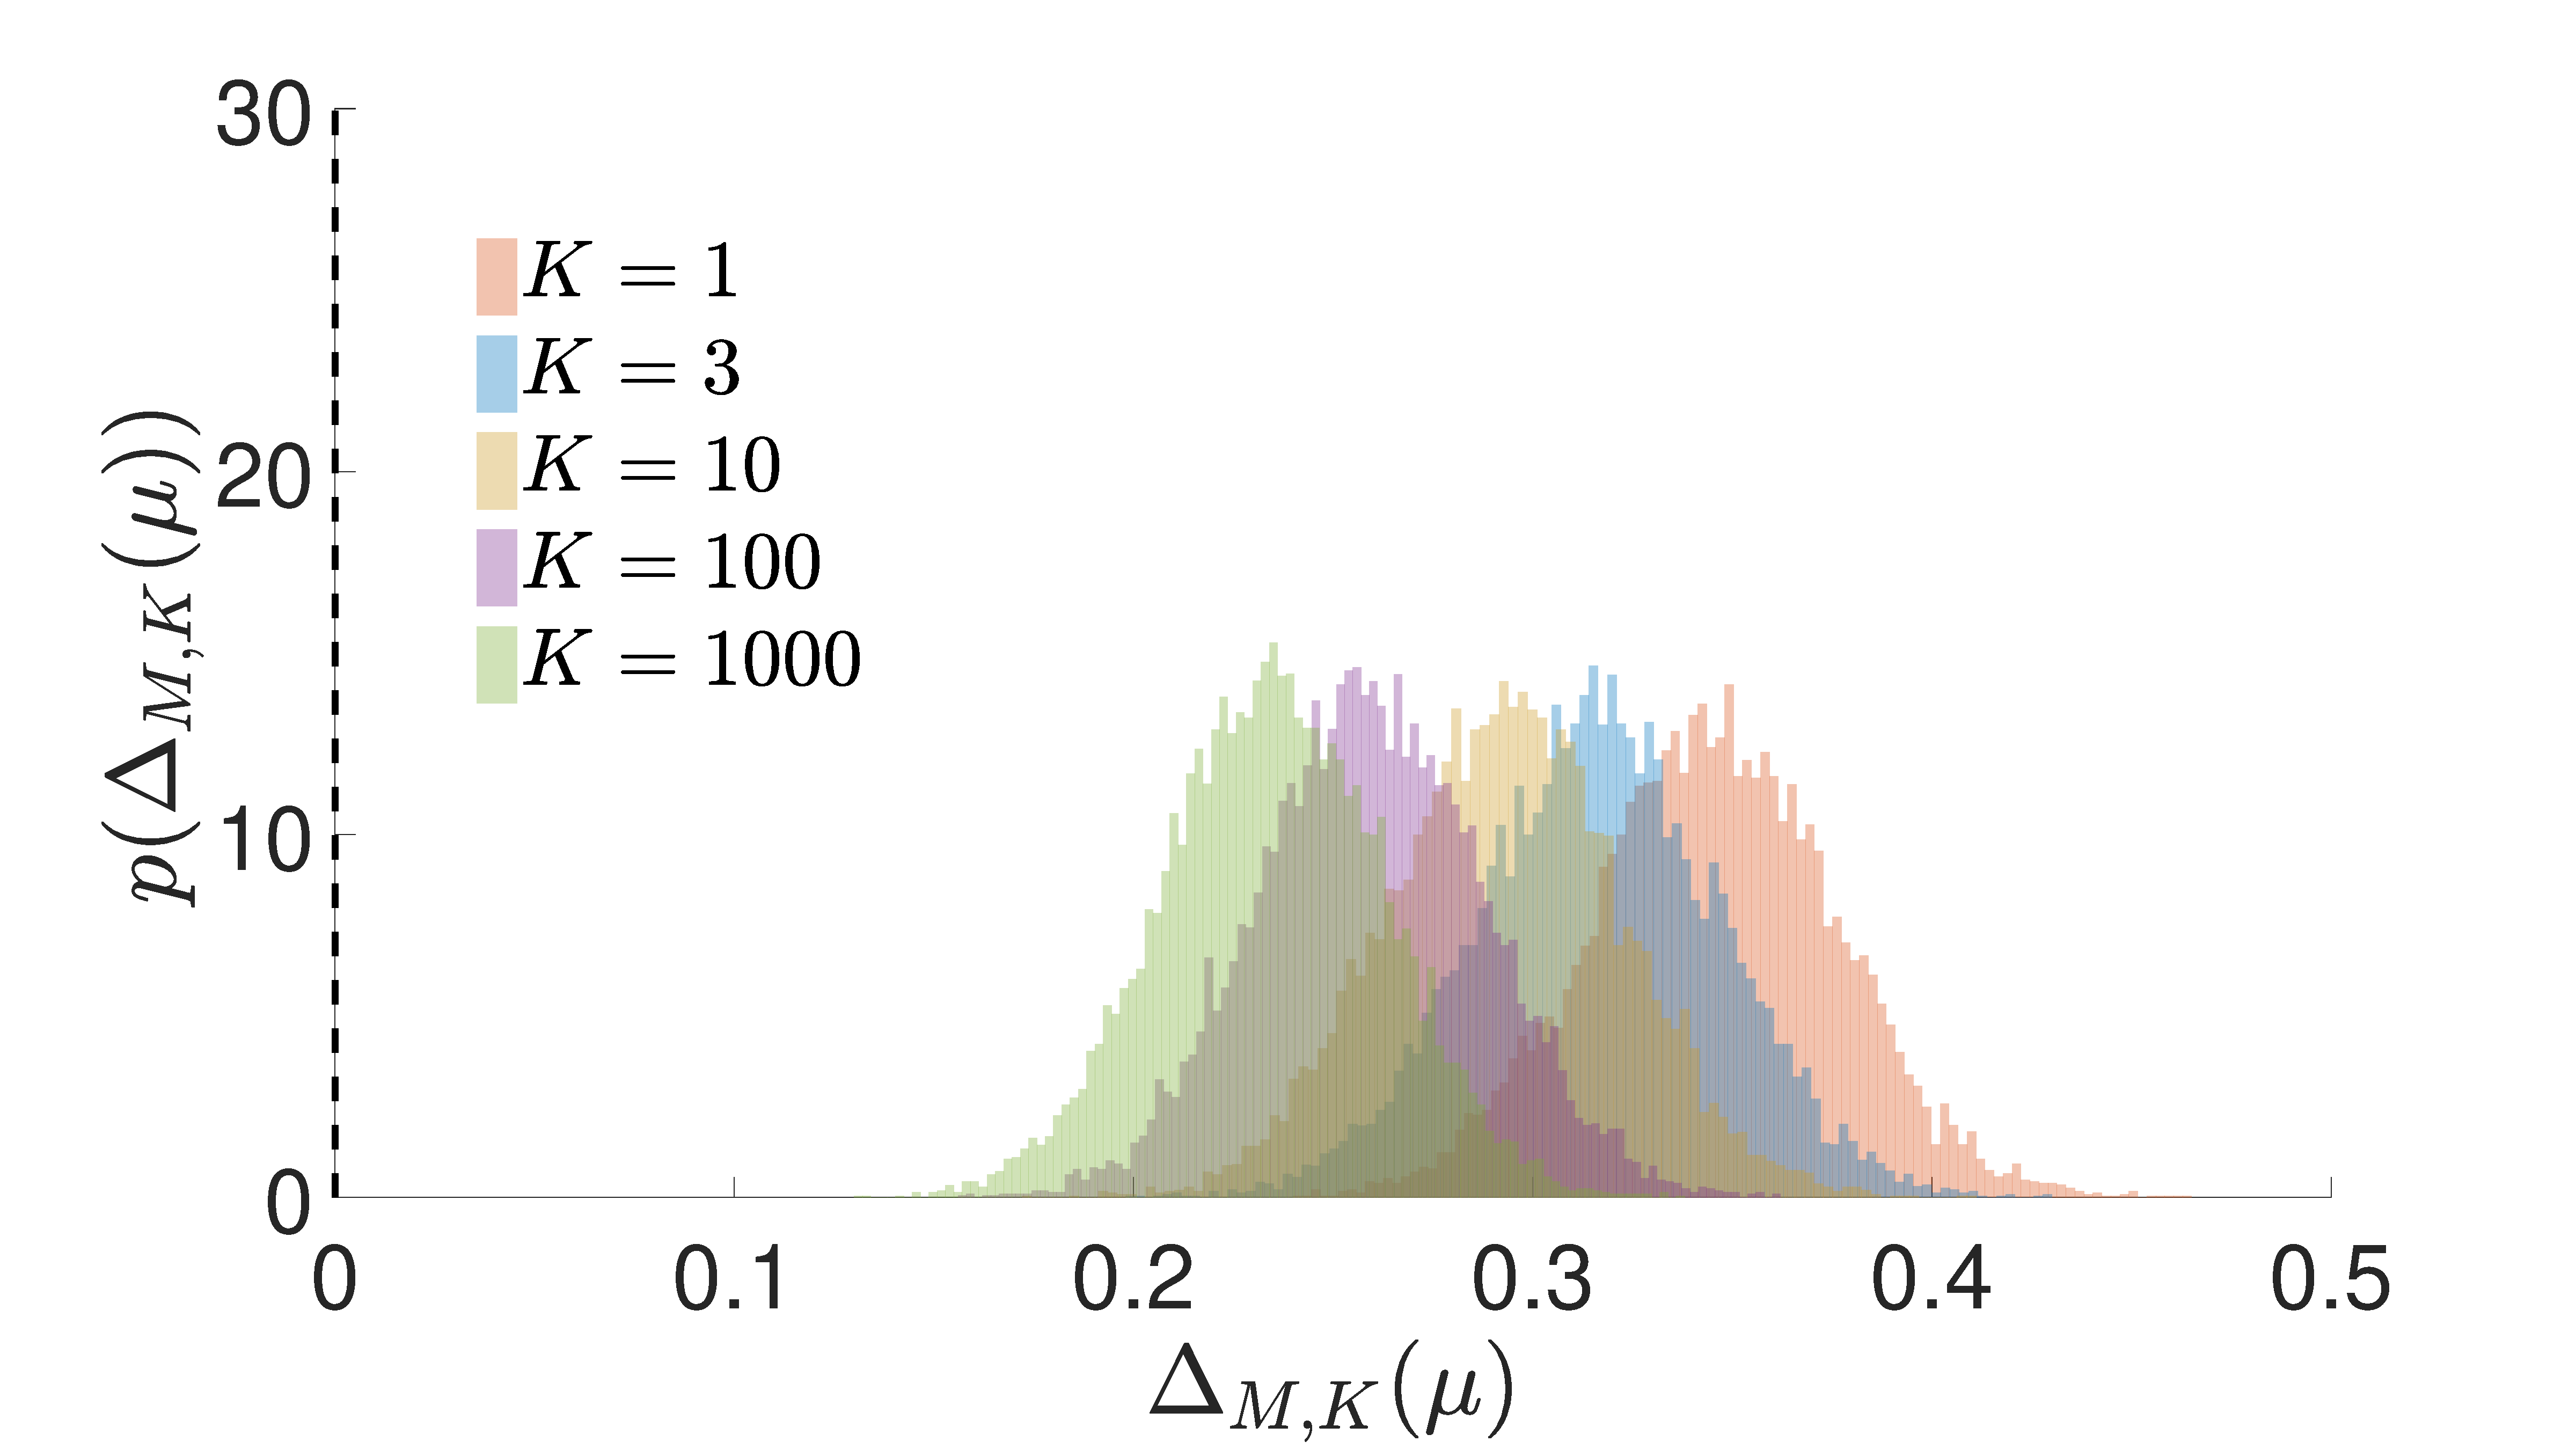
\includegraphics[width=\textwidth]{hv_mu_hist_IWAE}
		\caption{\gls{IWAE} generative network gradient estimates \label{fig:hv/mu_hist_iwae}}
	\end{subfigure} ~~~~~~~~~~
	\begin{subfigure}[b]{0.45\textwidth}
		\centering
		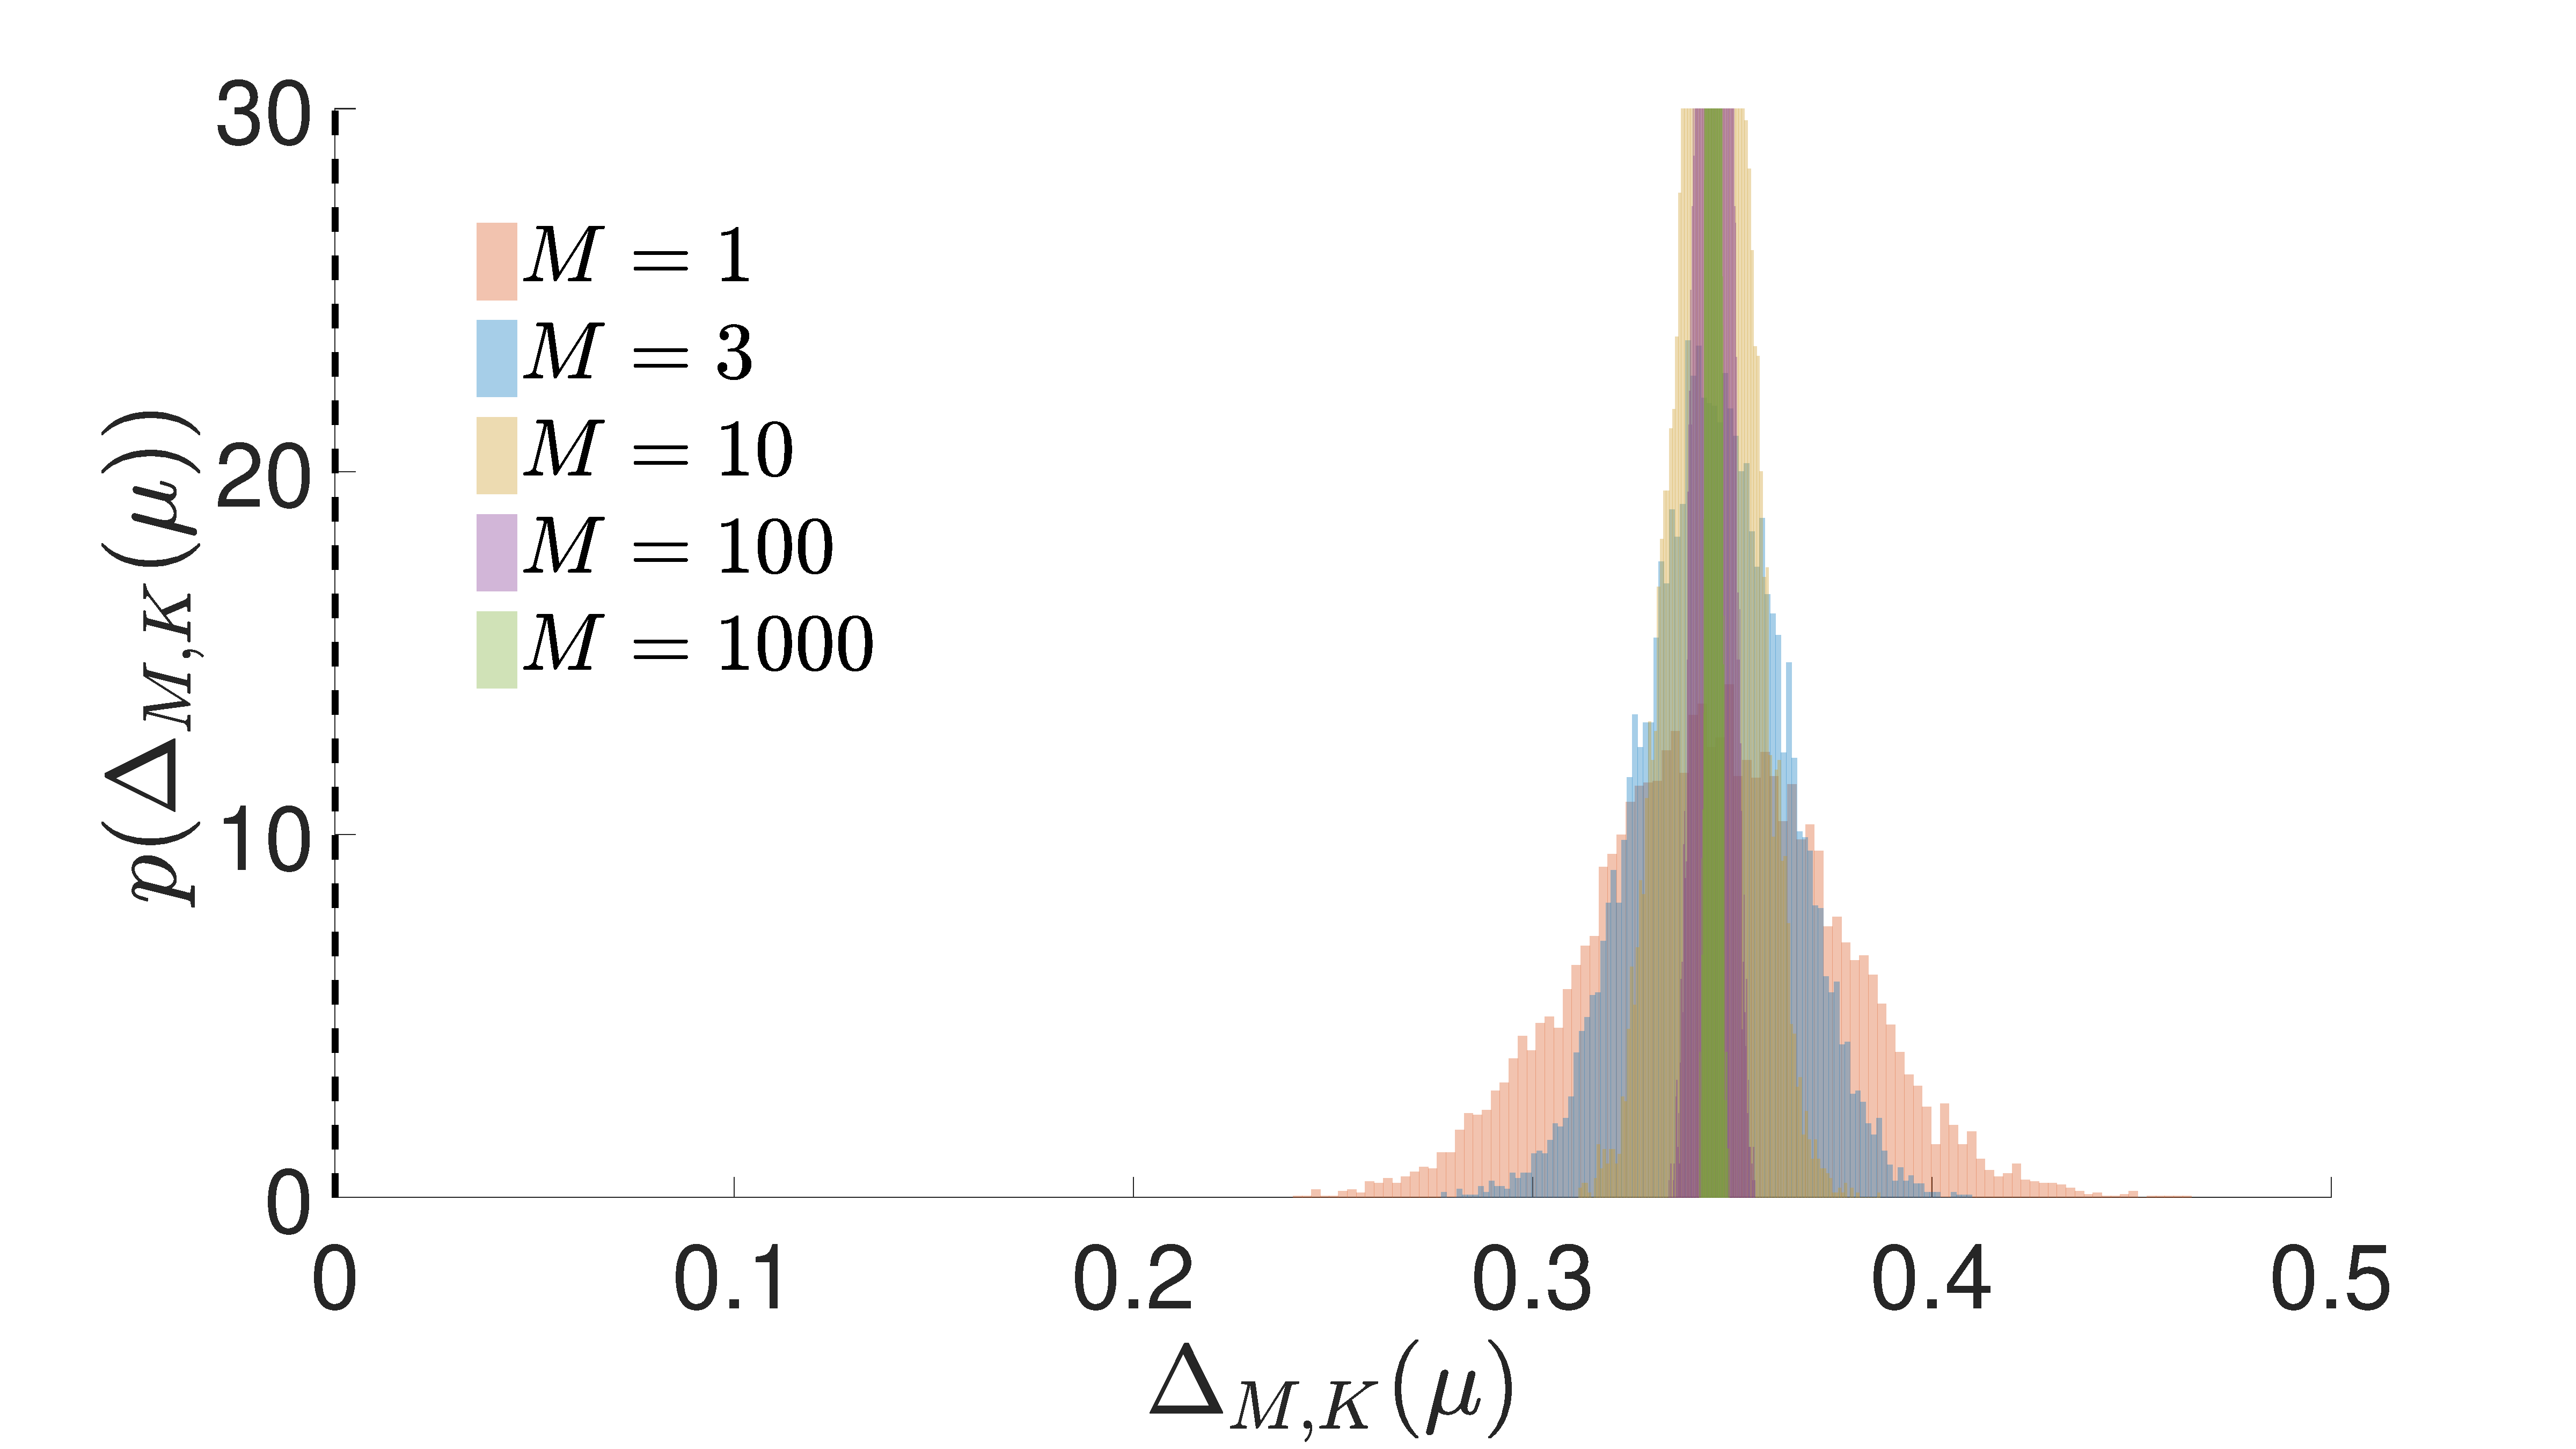
\includegraphics[width=\textwidth]{hv_mu_hist_VAE}
		\caption{\gls{VAE} generative network gradient estimates \label{fig:hv/mu_hist_vae}}
	\end{subfigure}
	\caption{Histograms of gradient estimates as per Figure~\ref{fig:snr/hists}.
		\label{fig:hv/hists}
	\vspace{-4pt}}
\end{figure}

\begin{figure}[h]
	\centering
	\begin{subfigure}[b]{0.45\textwidth}
		\centering
		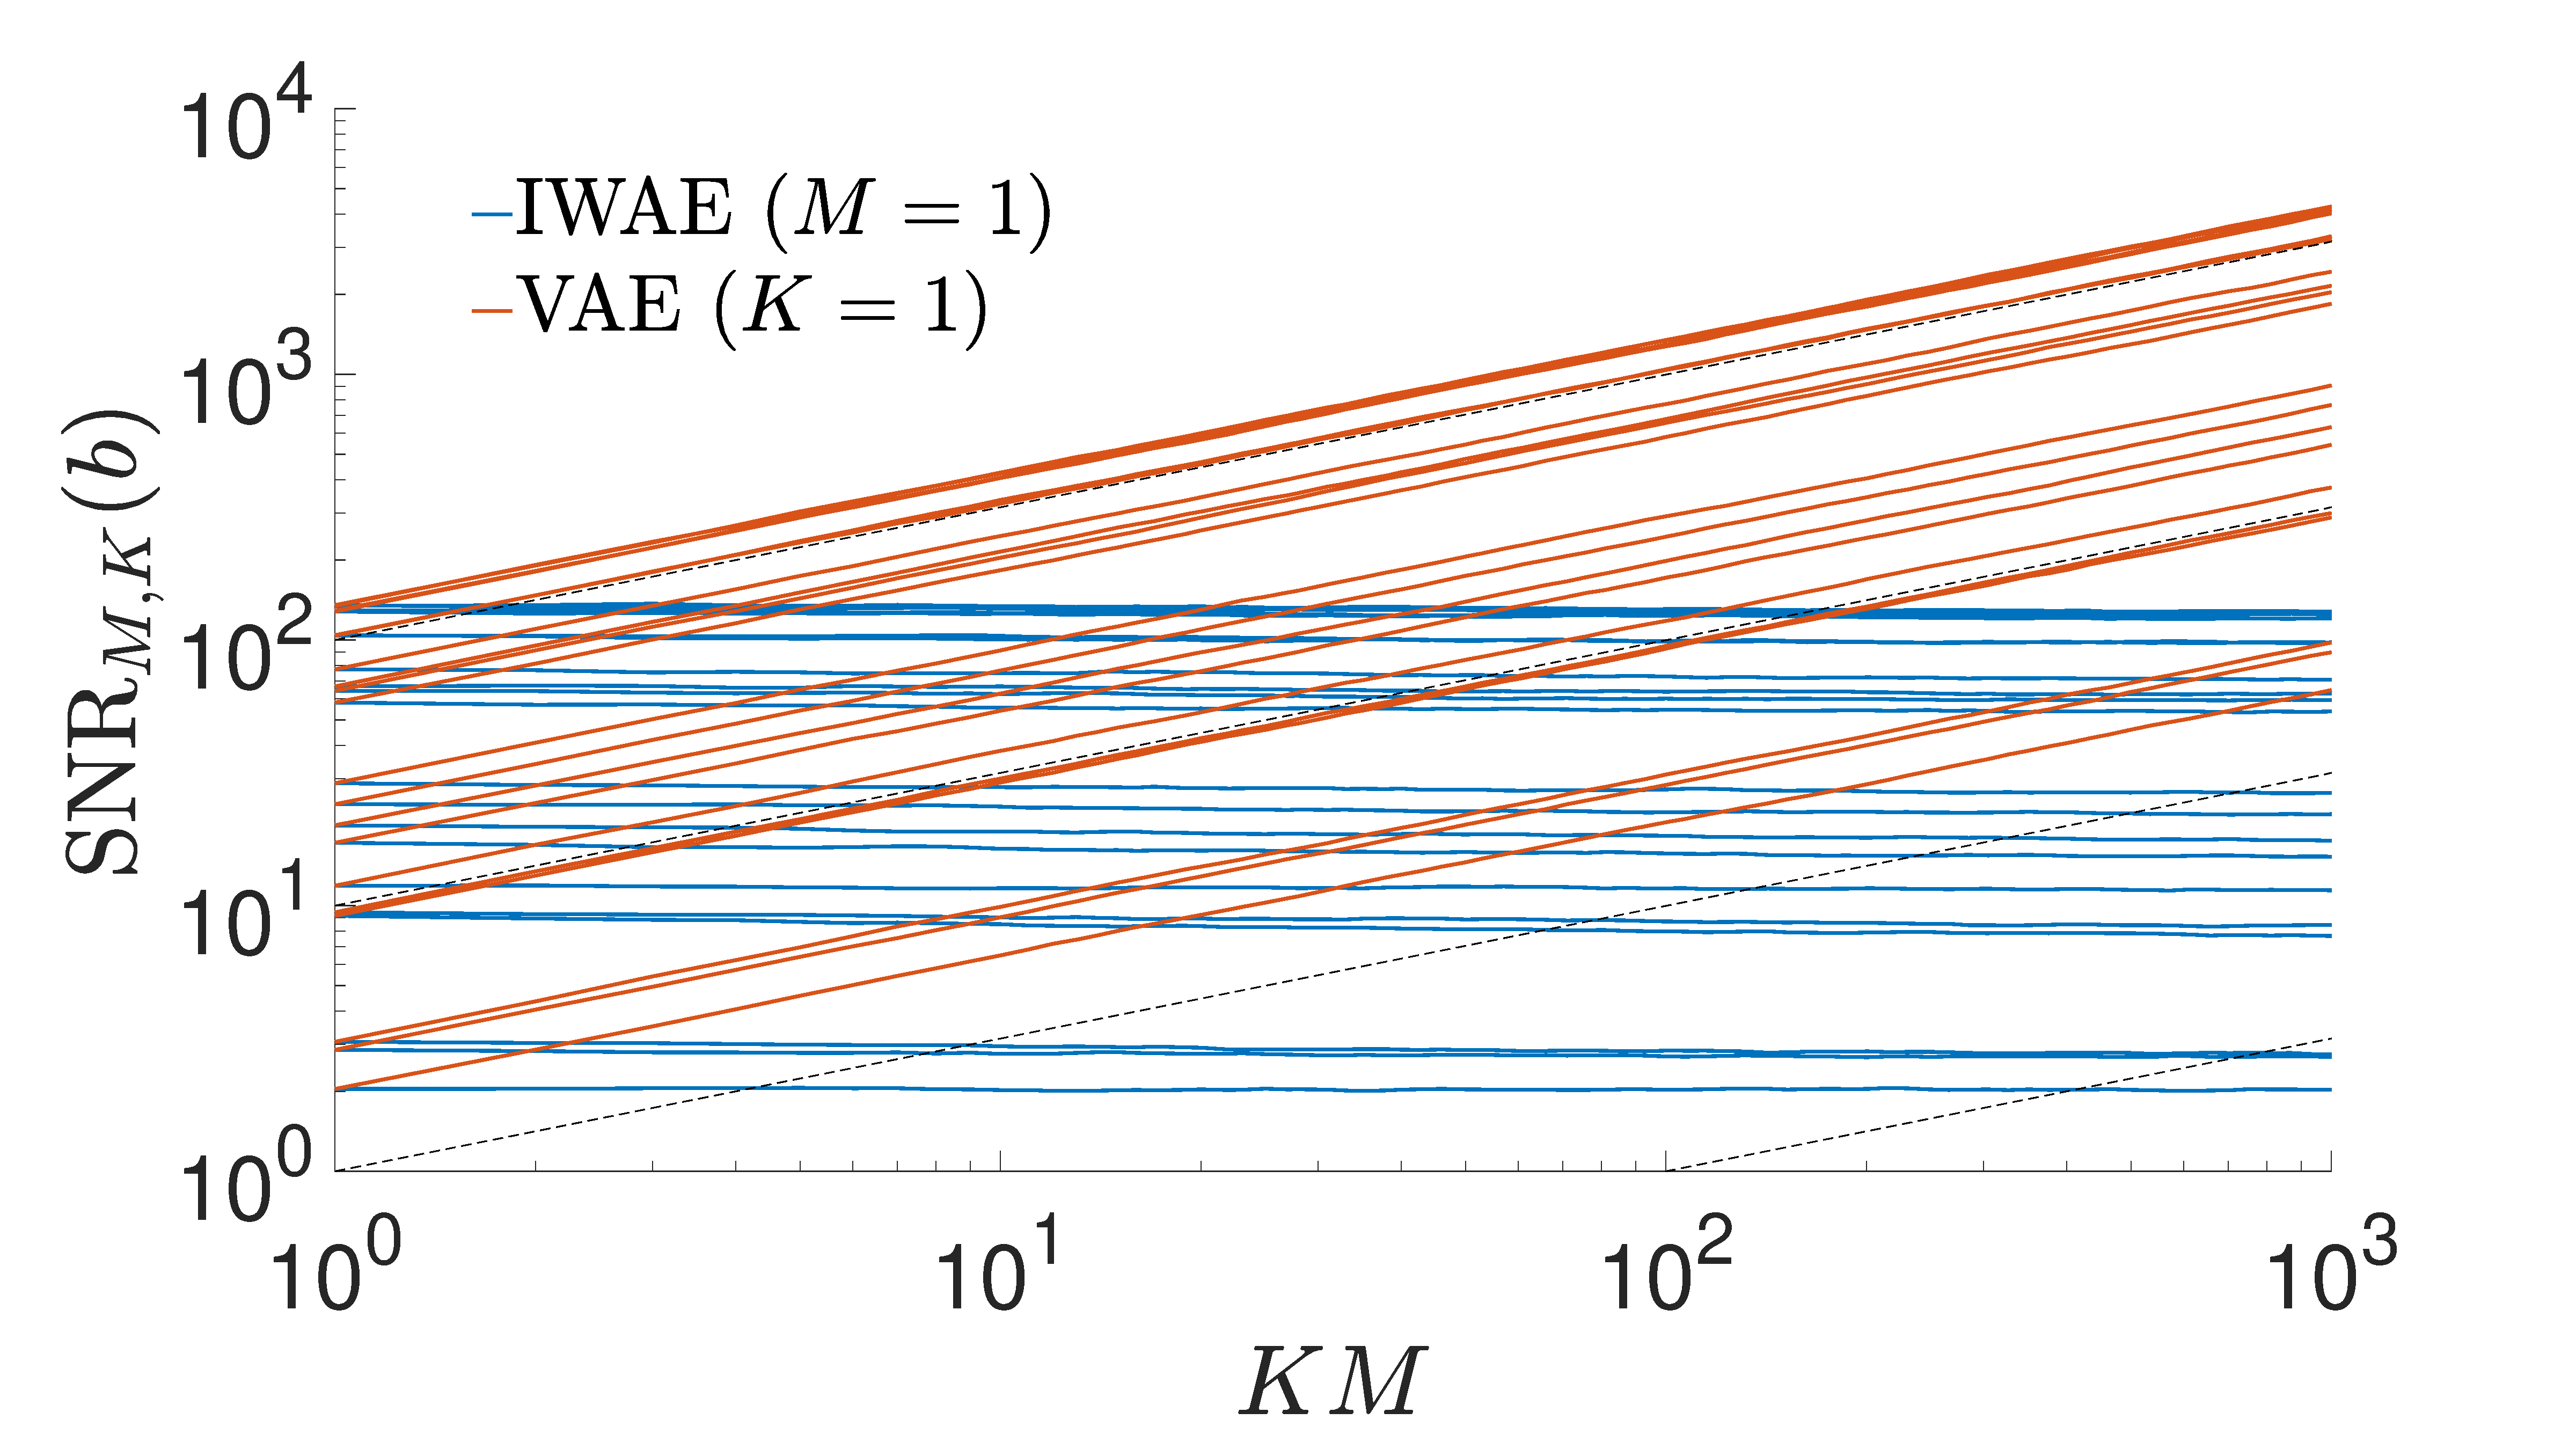
\includegraphics[width=\textwidth]{hv_b_conv}
		\caption{Convergence of \gls{SNR} for inference network \label{fig:hv/b}}
	\end{subfigure} ~~~~~~~~~~
	\begin{subfigure}[b]{0.45\textwidth}
		\centering
		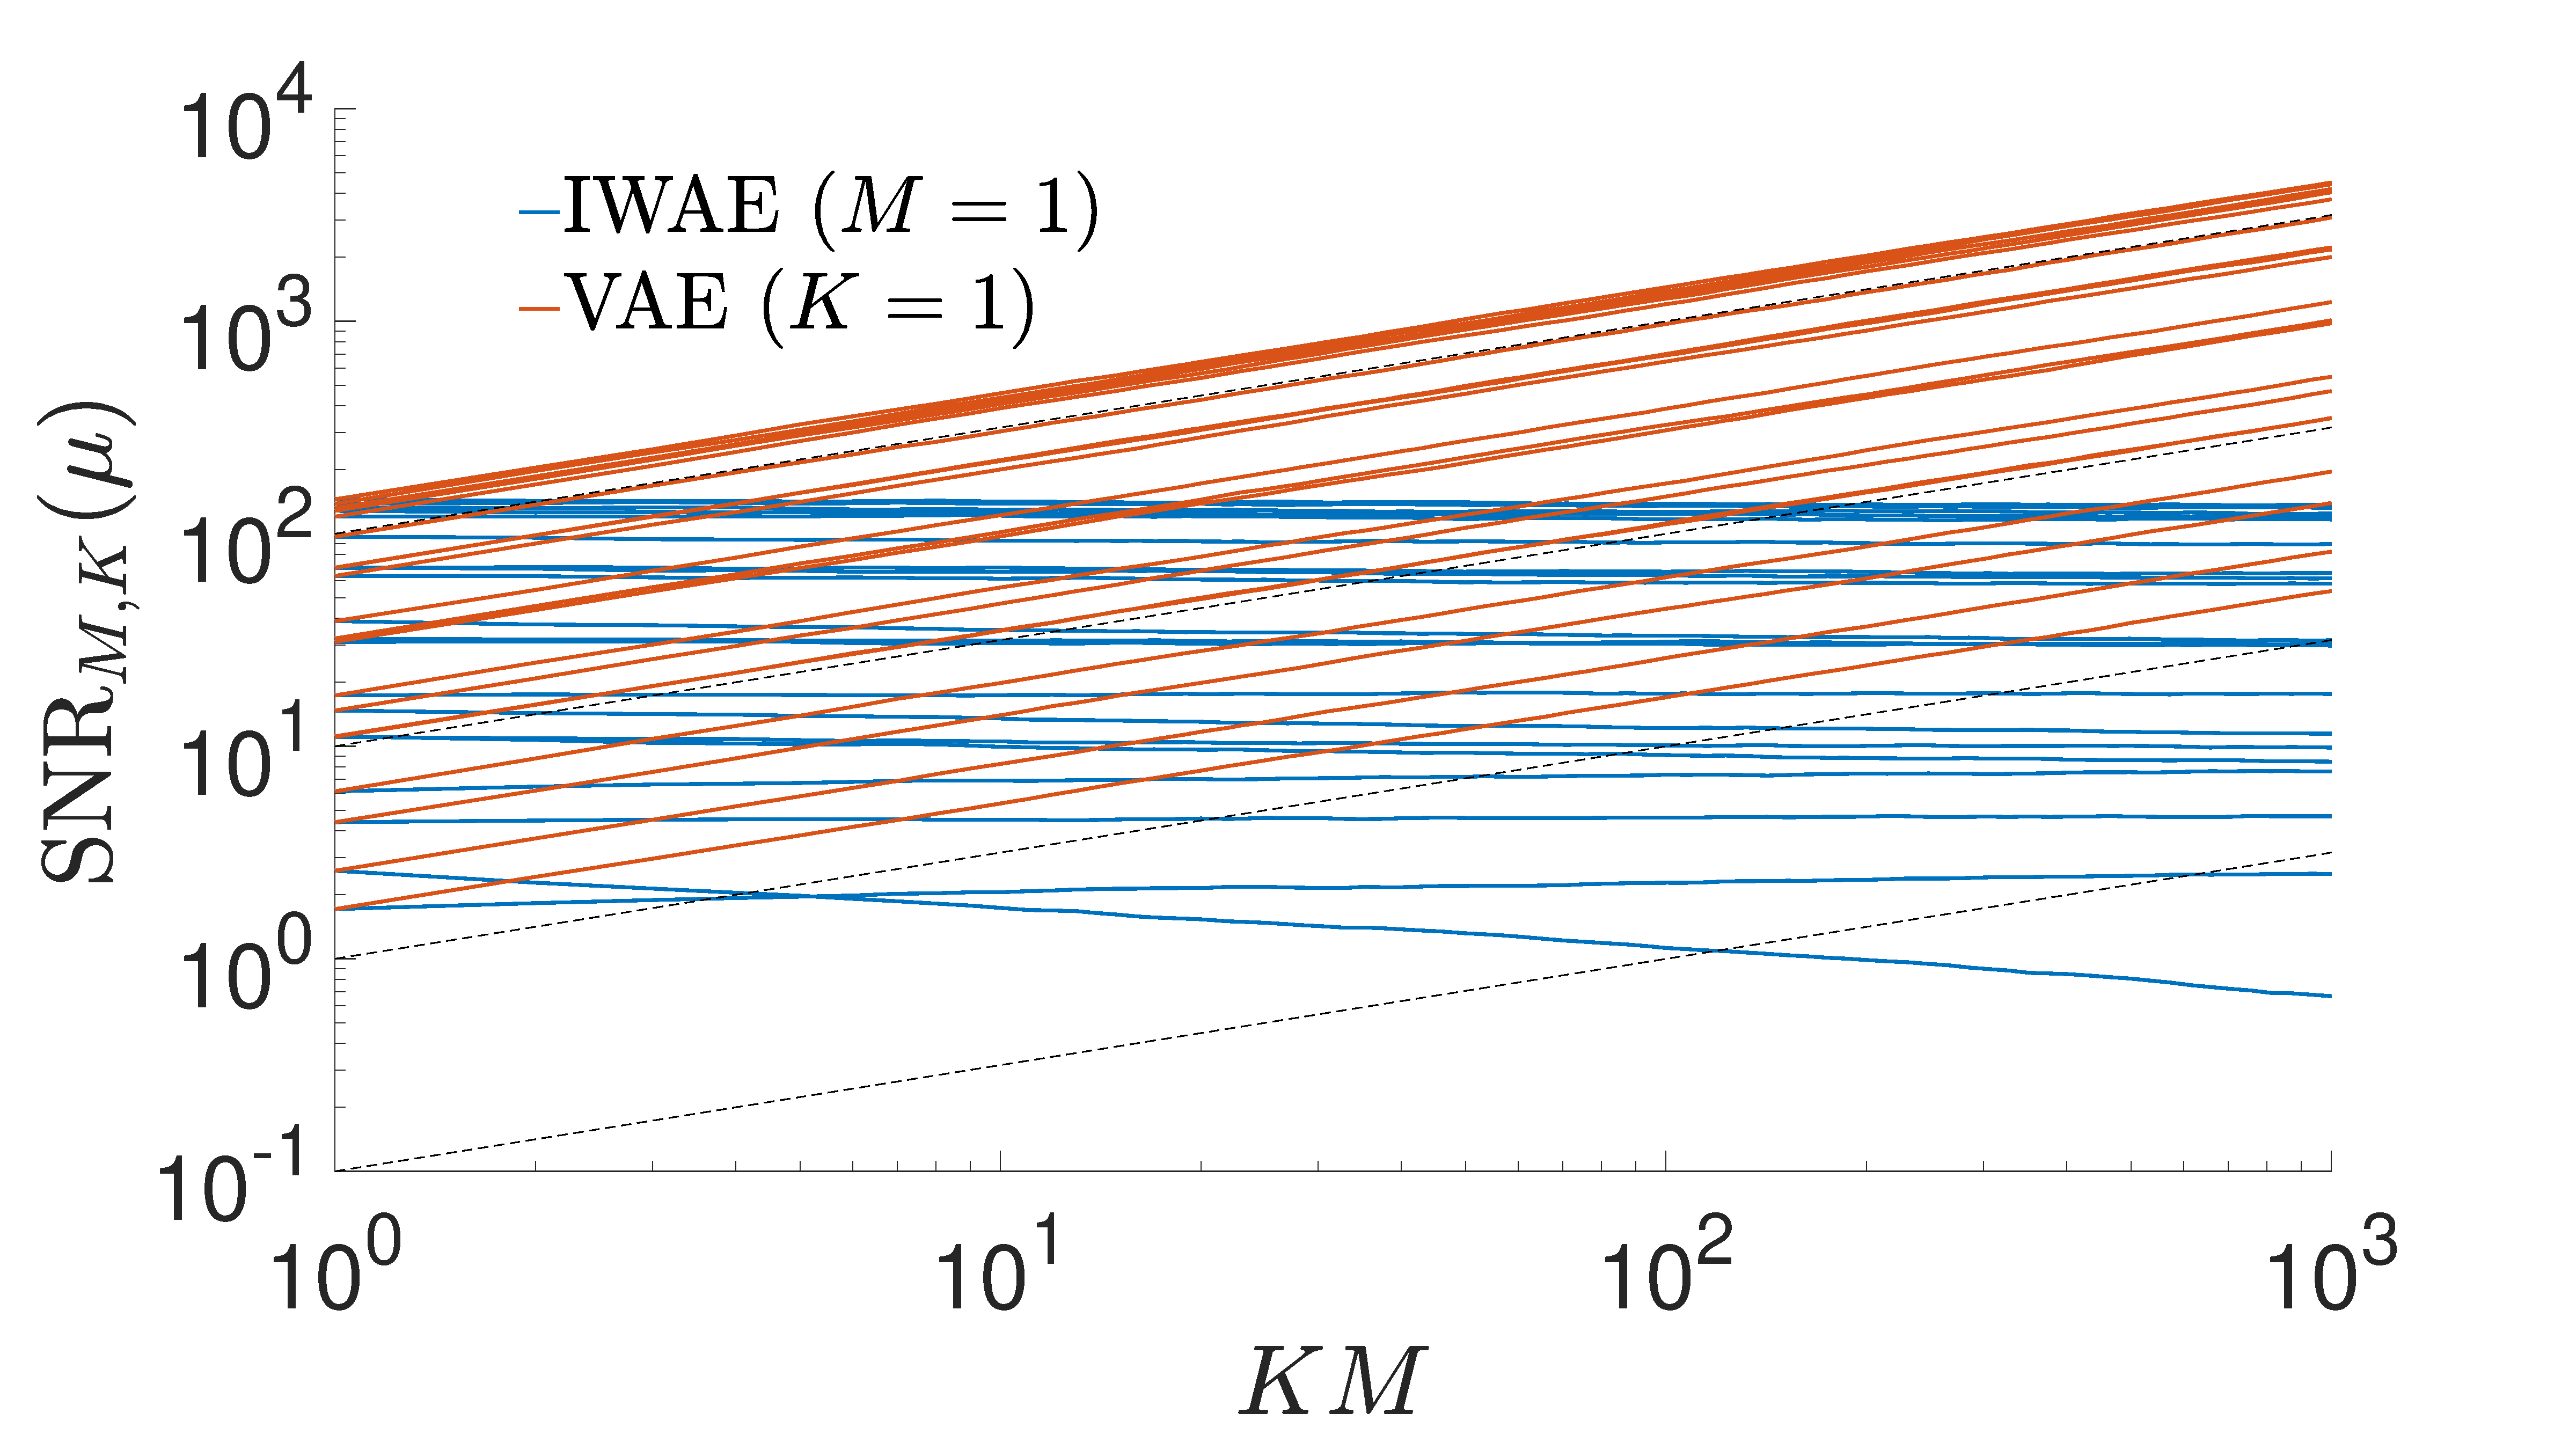
\includegraphics[width=\textwidth]{hv_mu_conv}
		\caption{Convergence of \gls{SNR} for generative network\label{fig:hv/mu}}
	\end{subfigure}
	\caption{Convergence of signal-to-noise ratios of gradient estimates
		as per Figure~\ref{fig:snr/K_conv}.
		\label{fig:hv/K_conv}}
\end{figure}


\begin{figure}[h]
	\centering
	\begin{subfigure}[b]{0.45\textwidth}
		\centering
		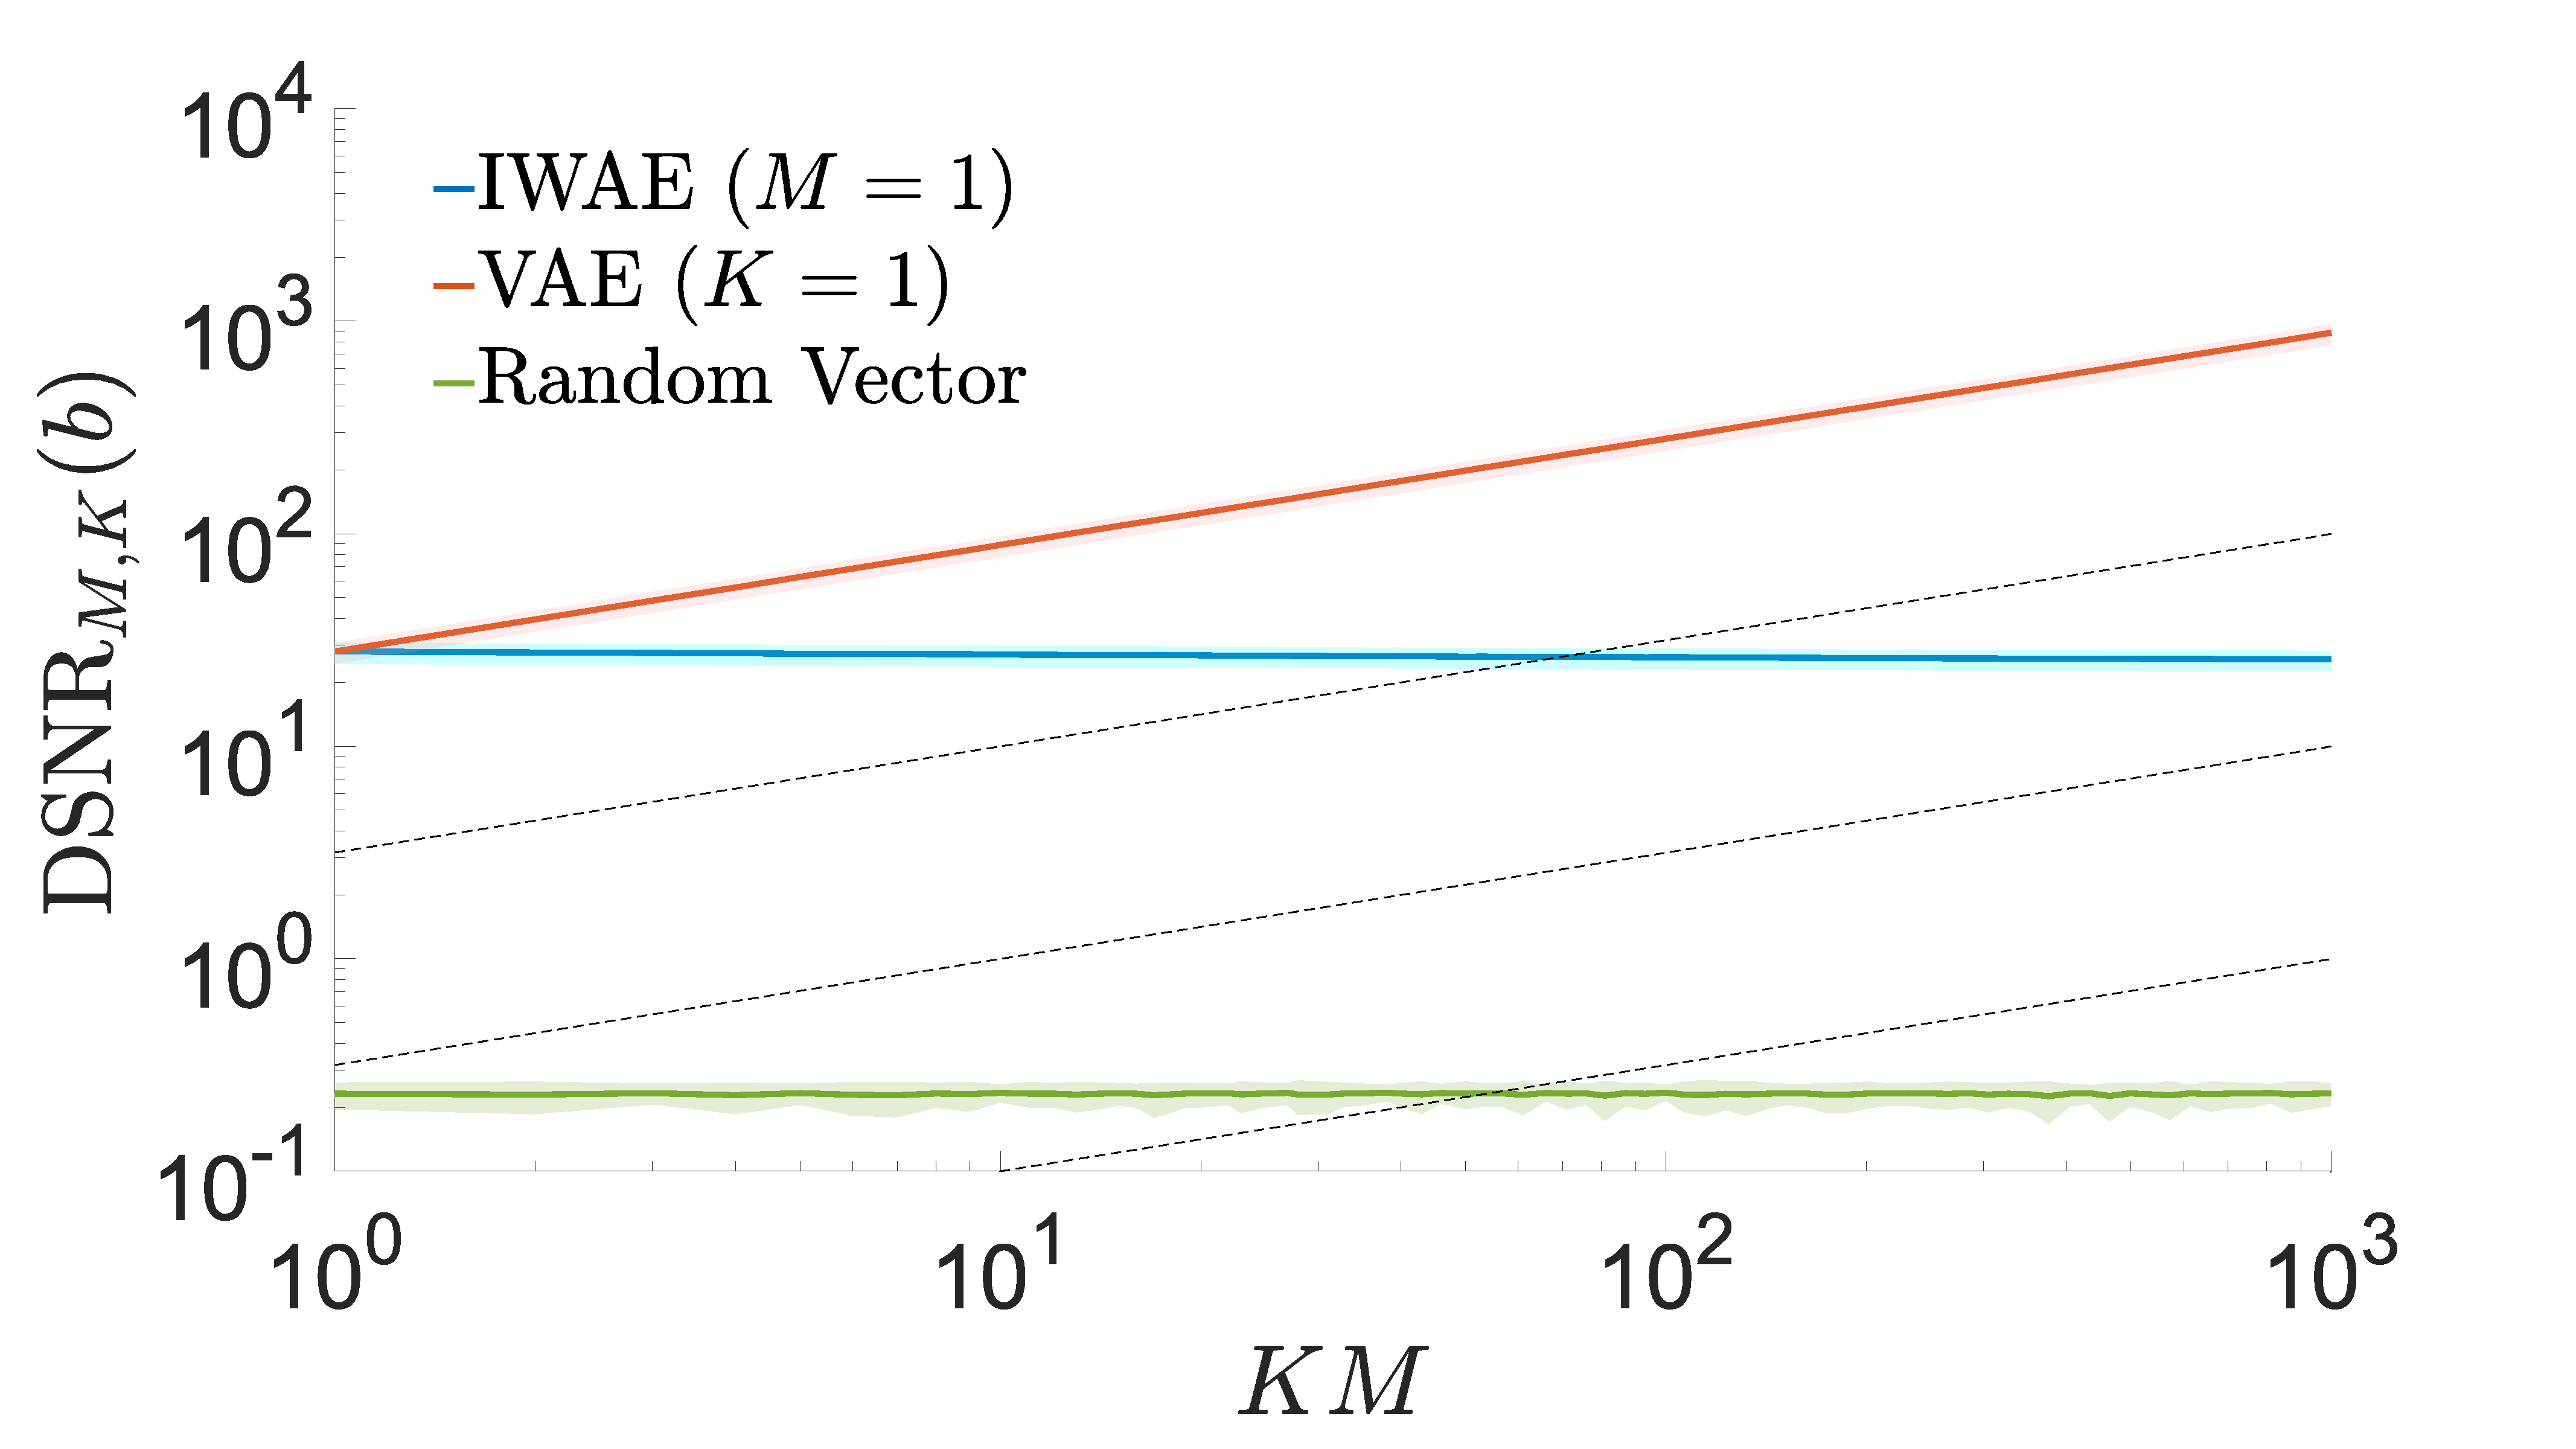
\includegraphics[width=\textwidth]{hv_snr_dir}
		\caption{Convergence of \textsc{dsnr} for inference network\label{fig:hv/snr_dir}}
	\end{subfigure}~~~~~~~~~~
	\begin{subfigure}[b]{0.45\textwidth}
		\centering
		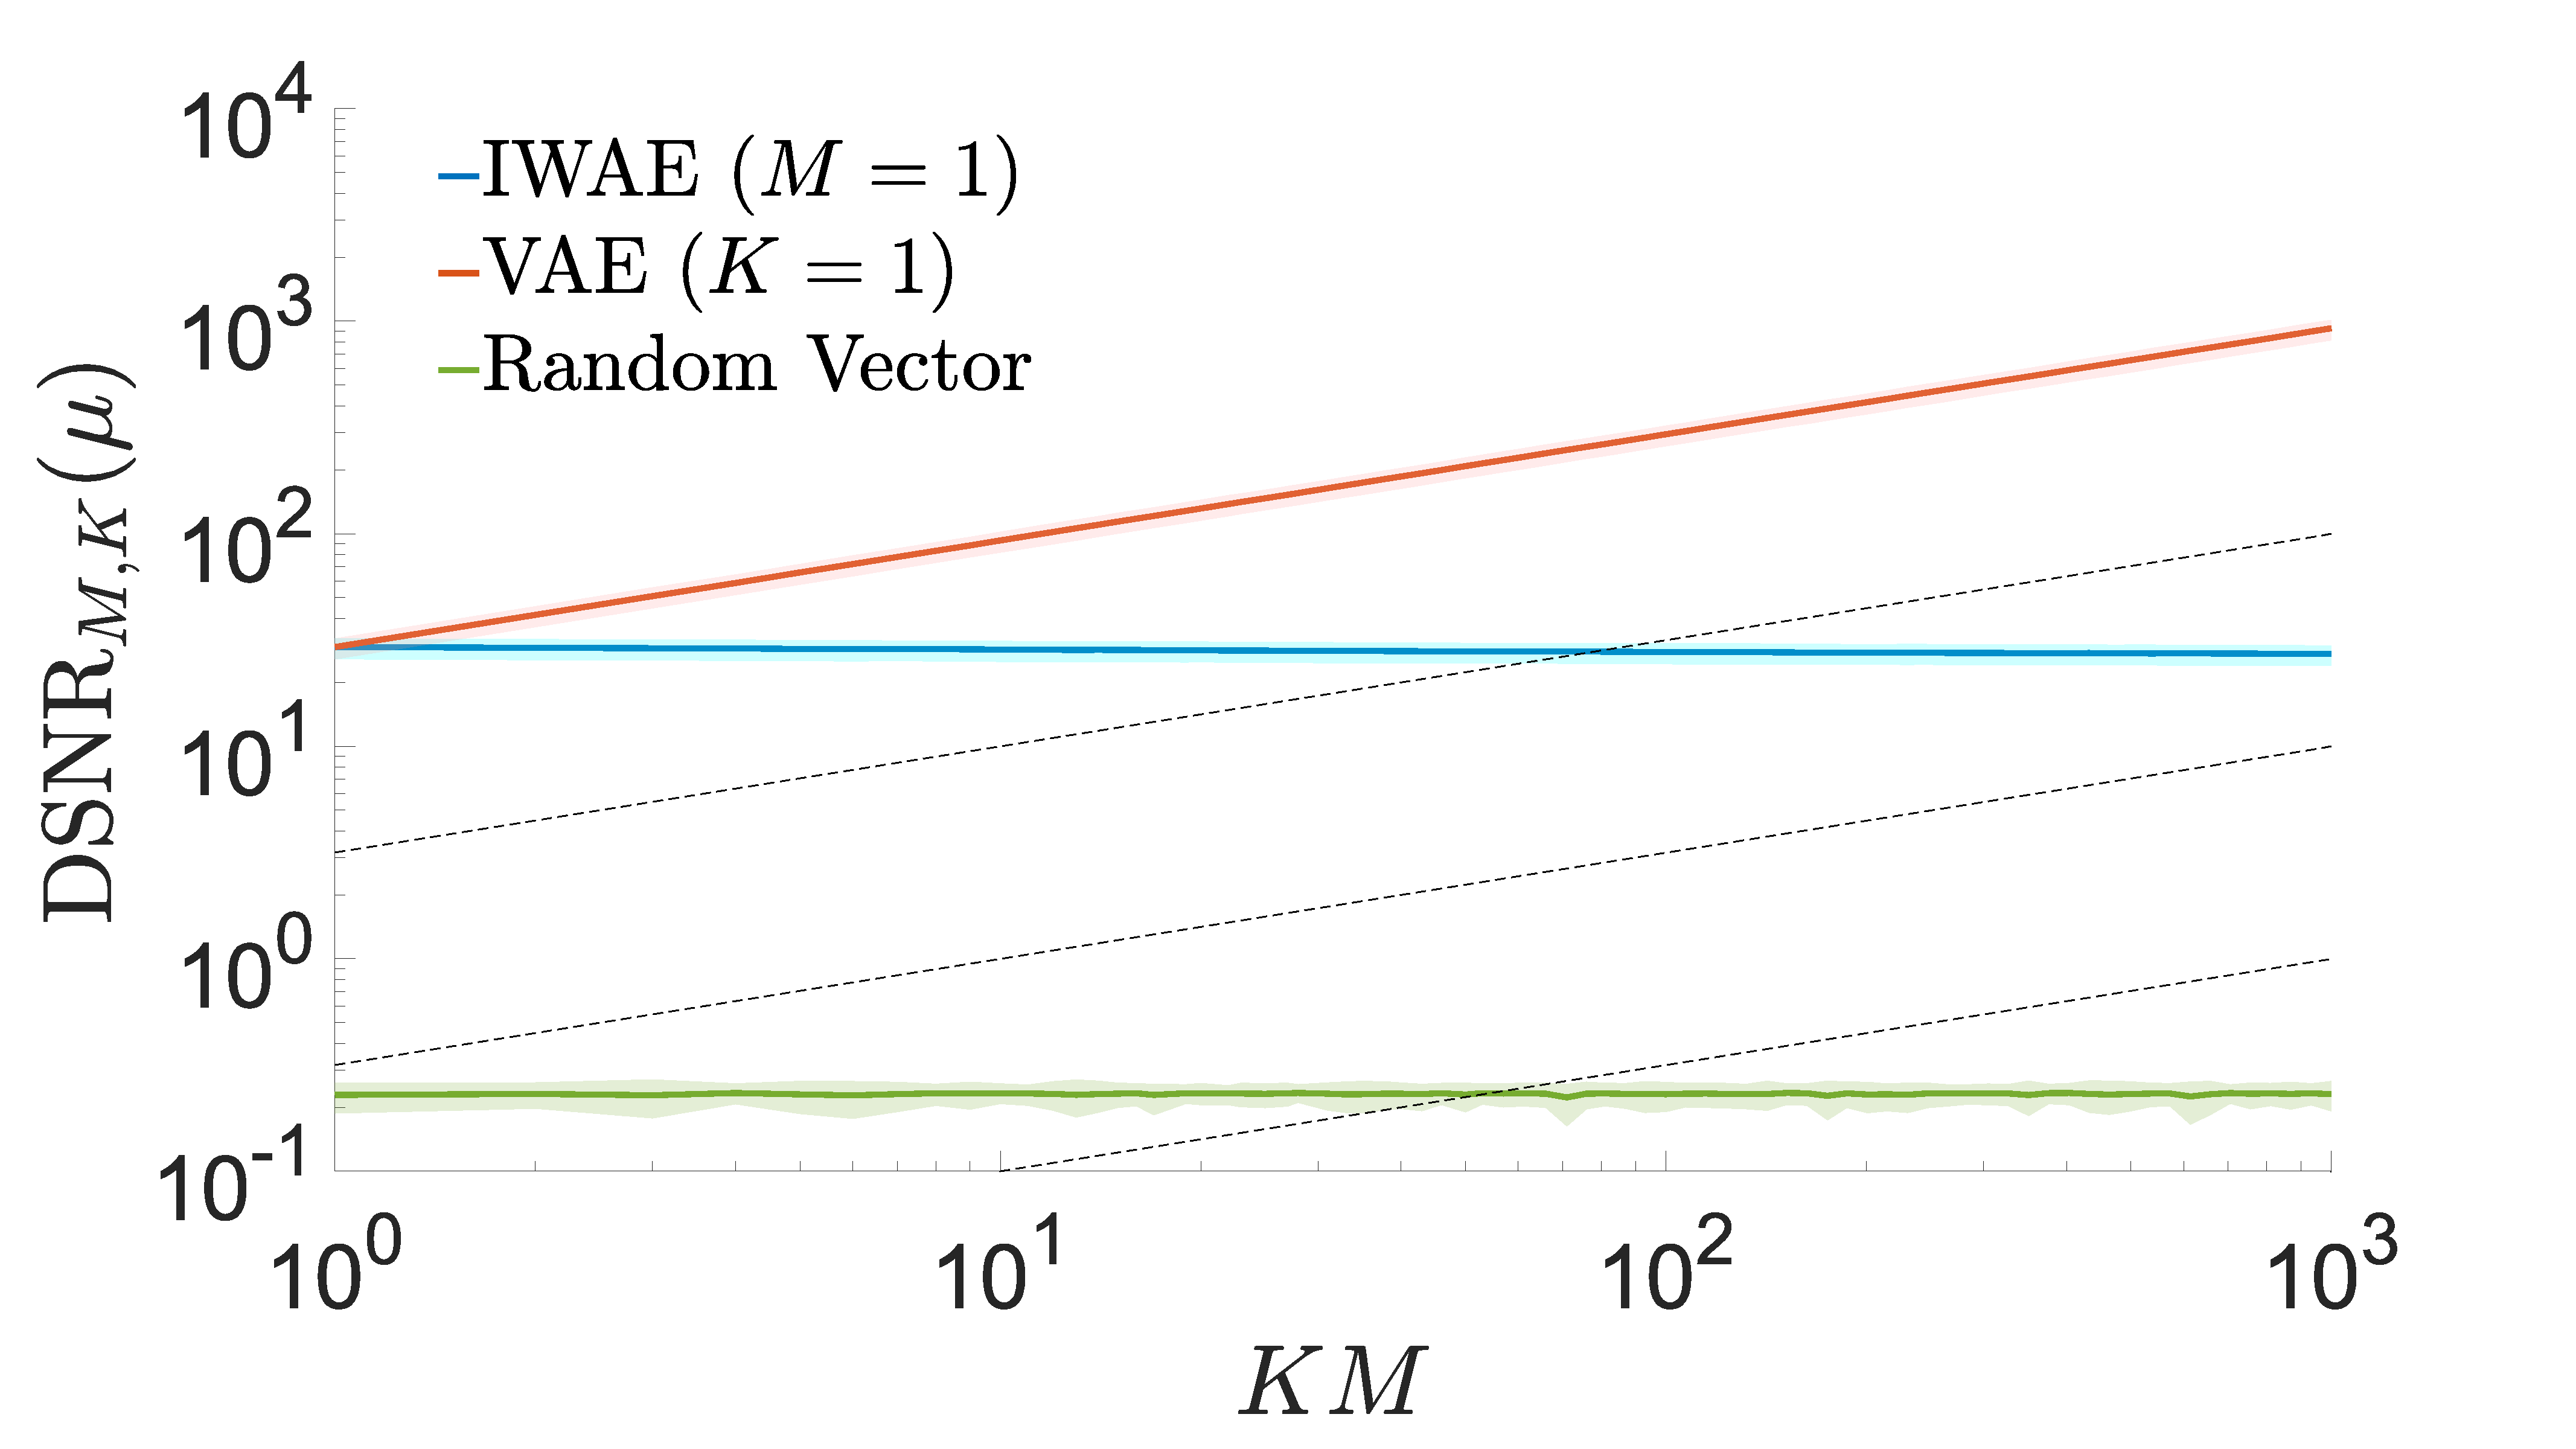
\includegraphics[width=\textwidth]{hv_snr_dir_mu}
		\caption{Convergence of \textsc{dsnr} for generative network\label{fig:hv/snr_dir_mu}}
	\end{subfigure}
	\caption{Convergence of directional signal-to-noise ratio of gradients estimates 
		as per Figure~\ref{fig:snr/extra}.
		\label{fig:hv/extra_end}}
\end{figure}

\begin{figure}[h]
	\centering
	\begin{subfigure}[b]{0.45\textwidth}
		\centering
		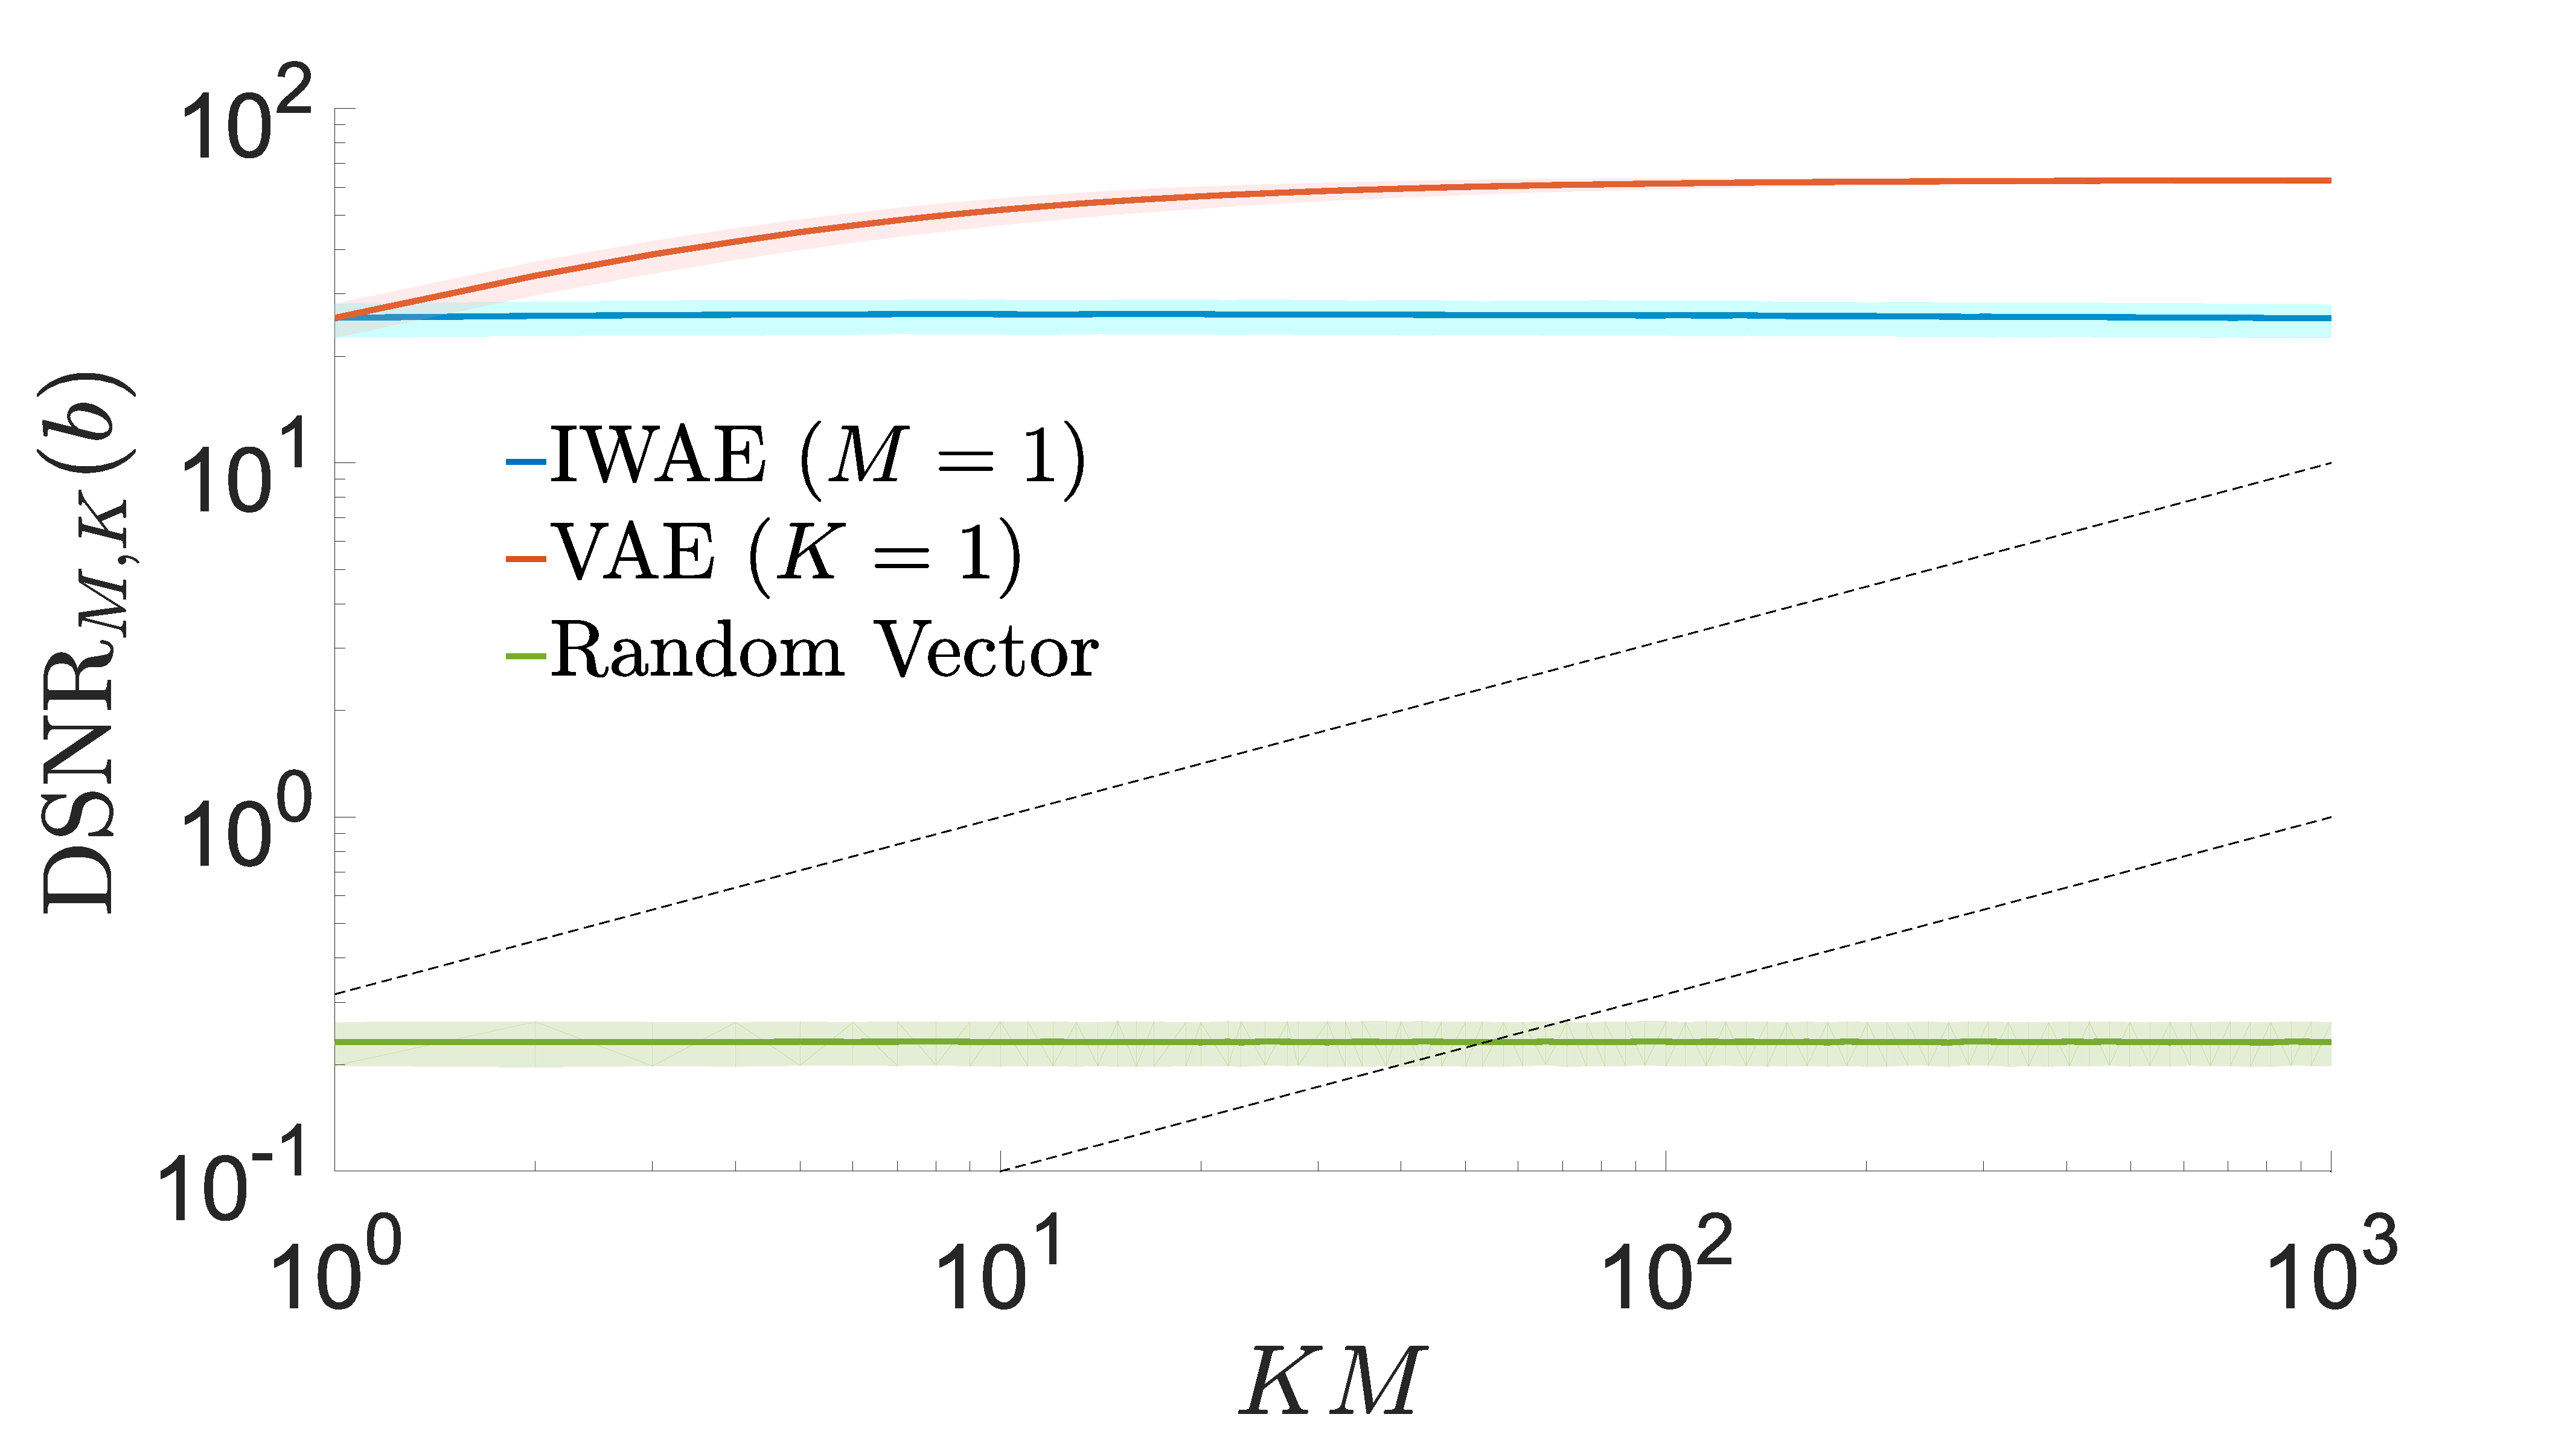
\includegraphics[width=\textwidth]{hv_dir_snr_end}
		\caption{Convergence of \textsc{dsnr} for inference network\label{fig:snr/hv_snr_dir_end}}
	\end{subfigure} ~~~~~~~~~~
	\begin{subfigure}[b]{0.45\textwidth}
		\centering
		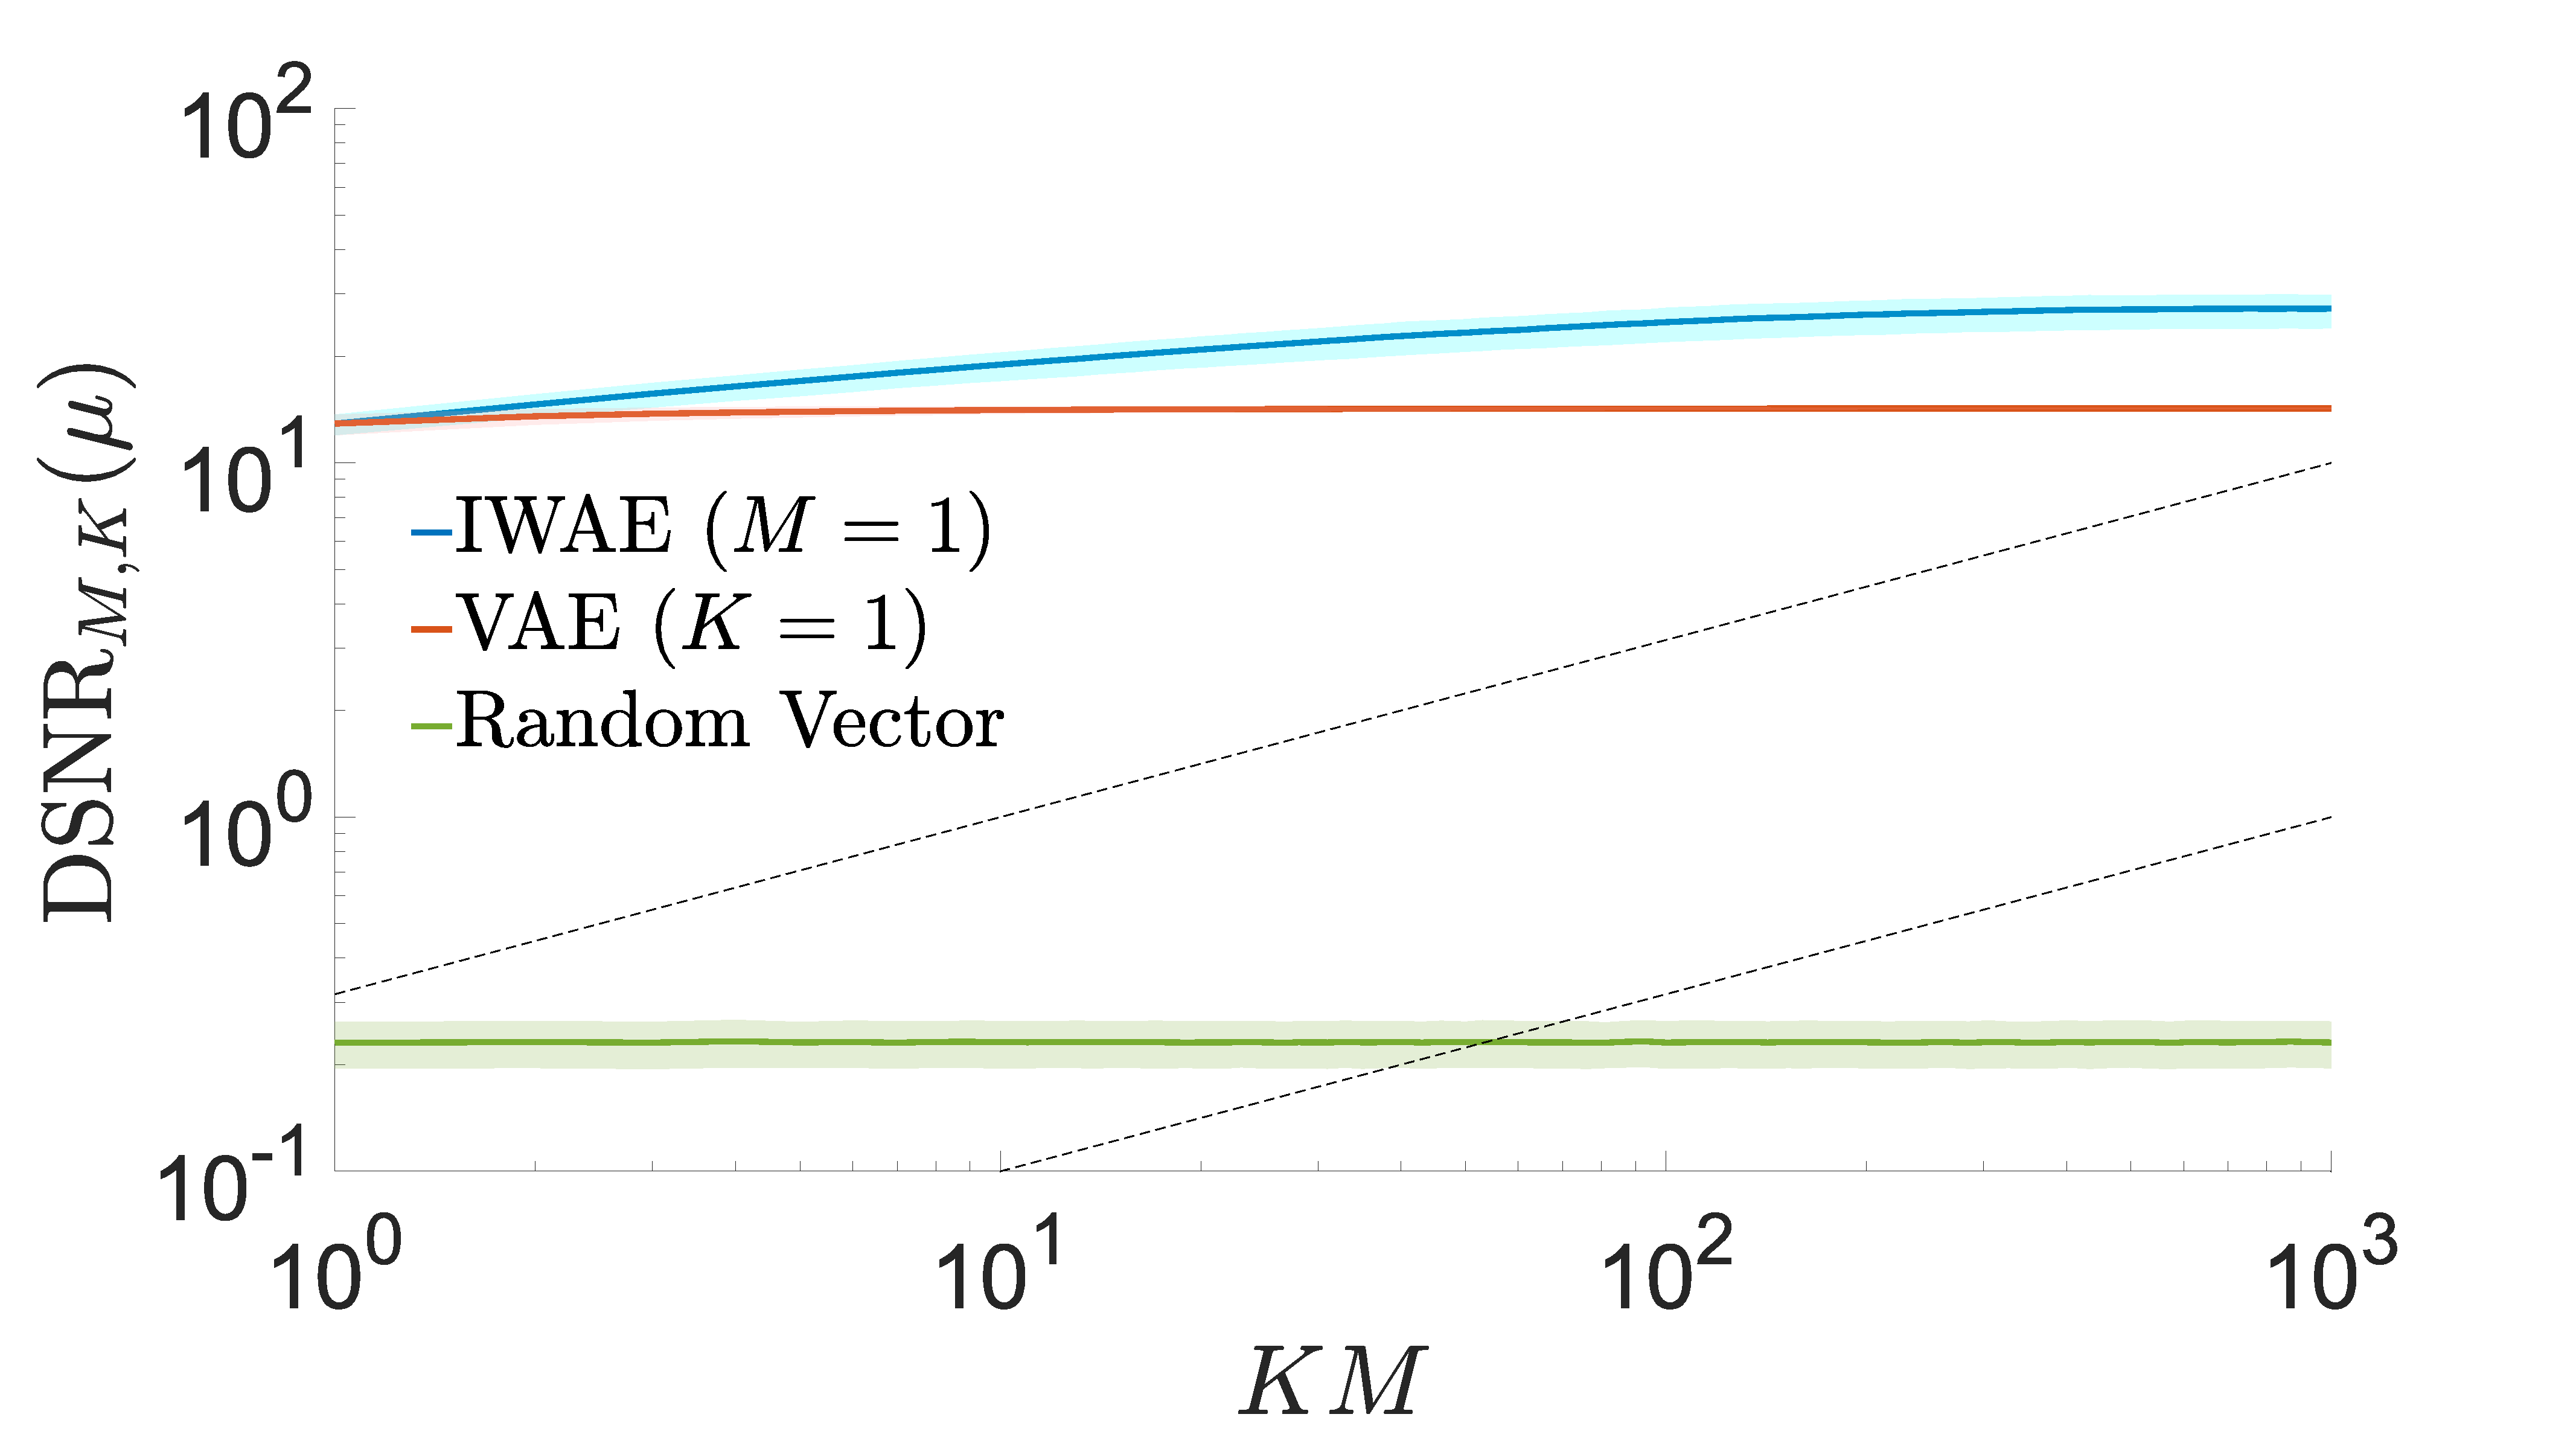
\includegraphics[width=\textwidth]{hv_dir_snr_mu_end}
		\caption{Convergence of \textsc{dsnr} for generative network\label{fig:snr/hv_snr_dir_mu_end}}
	\end{subfigure}
	\caption{Convergence of directional signal-to-noise ratio of gradient estimates where the
		true gradient is taken as $\E \left[\Delta_{1,1000}\right]$ as per
		Figure~\ref{fig:snr/extra_end}.
		\label{fig:snr/hv_extra_end}}
\end{figure}

\section{Convergence of Deep Generative Model for Alternative Parameter Settings}
\label{sec:app:exp-algs}

Figure~\ref{fig-app:mnistexpt/convergence} shows the convergence of the introduced algorithms under different
settings to those shown in Figure~\ref{fig:mnistexpt/convergence}. Namely we consider $M=4, K=16$ for~\gls{PIWAE} and~\gls{MIWAE} 
and $\beta = 0.05$ for~\gls{CIWAE}.  These settings all represent tighter bounds than those of the main paper.
Similar behavior is seen in terms of the~\gls{IWAE}-64 metric for all algorithms.  \gls{PIWAE} produced
similar mean behavior for all metrics, though the variance was noticeably increased for $\log \hat{p}(x)$.
For~\gls{CIWAE} and~\gls{MIWAE}, we see that the parameter settings represent an explicit trade-off between
the generative network and the inference network:  $\log \hat{p}(x)$ was noticeably increased for both, matching
that of~\gls{IWAE}, while $-\textsc{KL}(Q_{\phi}(z \given x) || P_{\theta}(z \given x))$ was reduced.
Critically, we see here that, as observed for~\gls{PIWAE} in the main paper,~\gls{MIWAE} and~\gls{CIWAE} are able to
match the generative model performance of~\gls{IWAE} whilst improving the KL metric, indicating that they have learned
better inference networks.

\begin{figure*}[h]
	\centering
   	\begin{subfigure}[b]{0.33\textwidth}
        \centering
        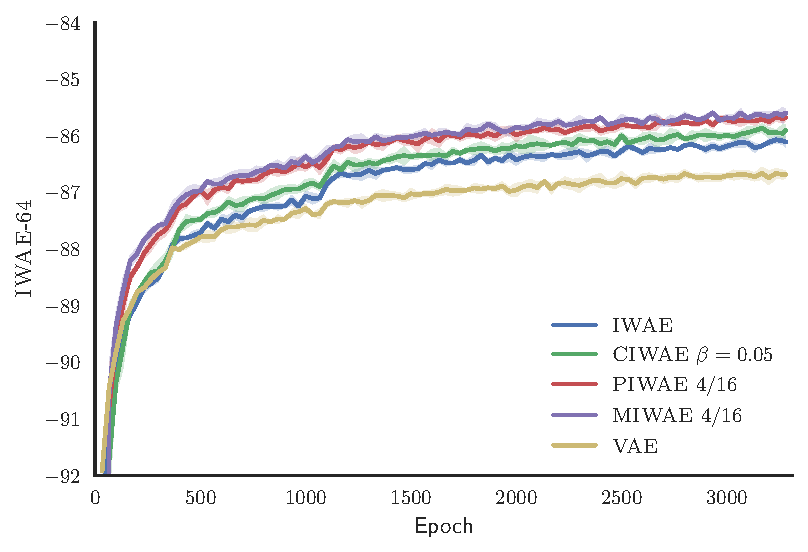
\includegraphics[width=\textwidth]{figures/tighter_bounds/optim_convergence_IWAE_64}
        \caption{\textsc{IWAE}$_{64}$ \label{fig-app:mnistexpt/convergence/iwae64}}
    \end{subfigure}
	\begin{subfigure}[b]{0.33\textwidth}
		\centering
		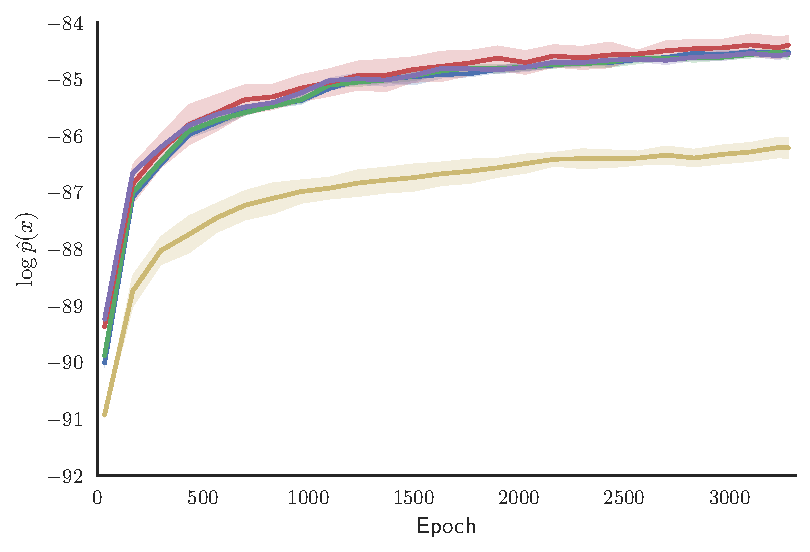
\includegraphics[width=\textwidth]{figures/tighter_bounds/optim_convergence_log_p(x)}
		\caption{$\log \hat{p}(x)$ \label{fig-app:mnistexpt/convergence/logpx}}
	\end{subfigure}
	\begin{subfigure}[b]{0.33\textwidth}
		\centering
		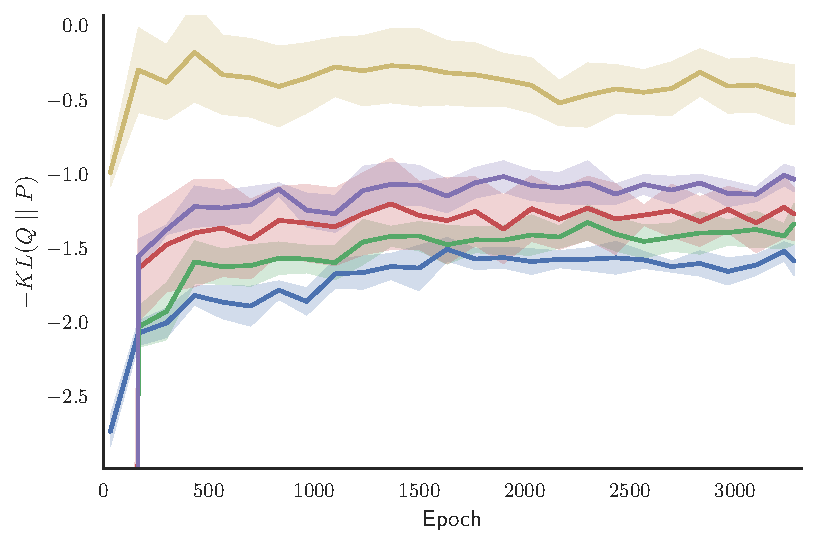
\includegraphics[width=\textwidth]{figures/tighter_bounds/optim_convergence_KL}
		\caption{$-\mathrm{KL}(Q_{\phi}(z \given x) || P_{\theta}(z \given x))$ \label{fig-app:mnistexpt/convergence/kl}}
	\end{subfigure}
	\caption{Convergence of different evaluation metrics for each method.  Plotting conventions as per
		 Figure~\ref{fig:mnistexpt/convergence}.
		\vspace{-12pt}  \label{fig-app:mnistexpt/convergence}}
\end{figure*}
% !Tex root=./tb_icml_2018.tex

\section{Convergence of Toy Gaussian Problem}
\label{sec:app:toy-Gauss}

We finish by assessing the effect of the outlined changes in the quality
of the gradient estimates on the final optimization for our toy Gaussian problem.  Figure~\ref{fig:snr/hd_gaussian}
shows the convergence of running Adam~\citep{Kingma2014adam} to optimize $\mu$, $A$, 
and $b$.  This suggests that the effects observed predominantly transfer to the overall
optimization problem.  Interestingly, setting $K=1$ and $M=1000$ gave the best performance
on learning not only the inference network parameters, but also the generative network
parameters.
\begin{figure*}[h]
	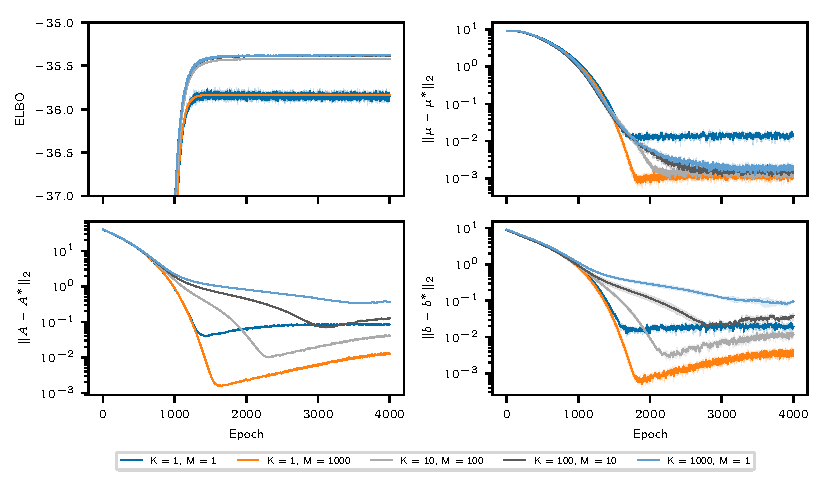
\includegraphics[width=\textwidth]{figures/tighter_bounds/hd_gaussian.pdf}
	\caption{Convergence of optimization for different values of $K$ and $M$. 
		\emph{(Top, left)} $\ELBO_{\text{IS}}$ during training
		(note this represents a different metric for different $K$). \emph{(Top, right)} $L_2$ distance of the generative network parameters from the true maximizer. \emph{(Bottom)} $L_2$ distance of the inference network parameters from the true maximizer. Plots show means over $3$ repeats with $\pm 1$ standard deviation. Optimization is performed using the Adam algorithm with all parameters initialized by sampling from the uniform distribution on $[1.5, 2.5]$.}
	\label{fig:snr/hd_gaussian}
\end{figure*}


\bibliography{refs}

%
%\section*{Acknowledgements}
%
%Tom Rainforth is supported by a BP industrial grant. Robert Cornish is supported by an NVIDIA scholarship. Frank Wood is supported under DARPA PPAML through the U.S. AFRL under Cooperative Agreement FA8750-14-2-0006, Sub Award number 61160290-111668.


\end{document}
